\chapter{RESULTADOS}


\begin{figure}[H]
    \centering
    \caption{Distribución de valores faltantes para la variable de Humedad Relativa (HR) en las 19 estaciones meteorológicas.}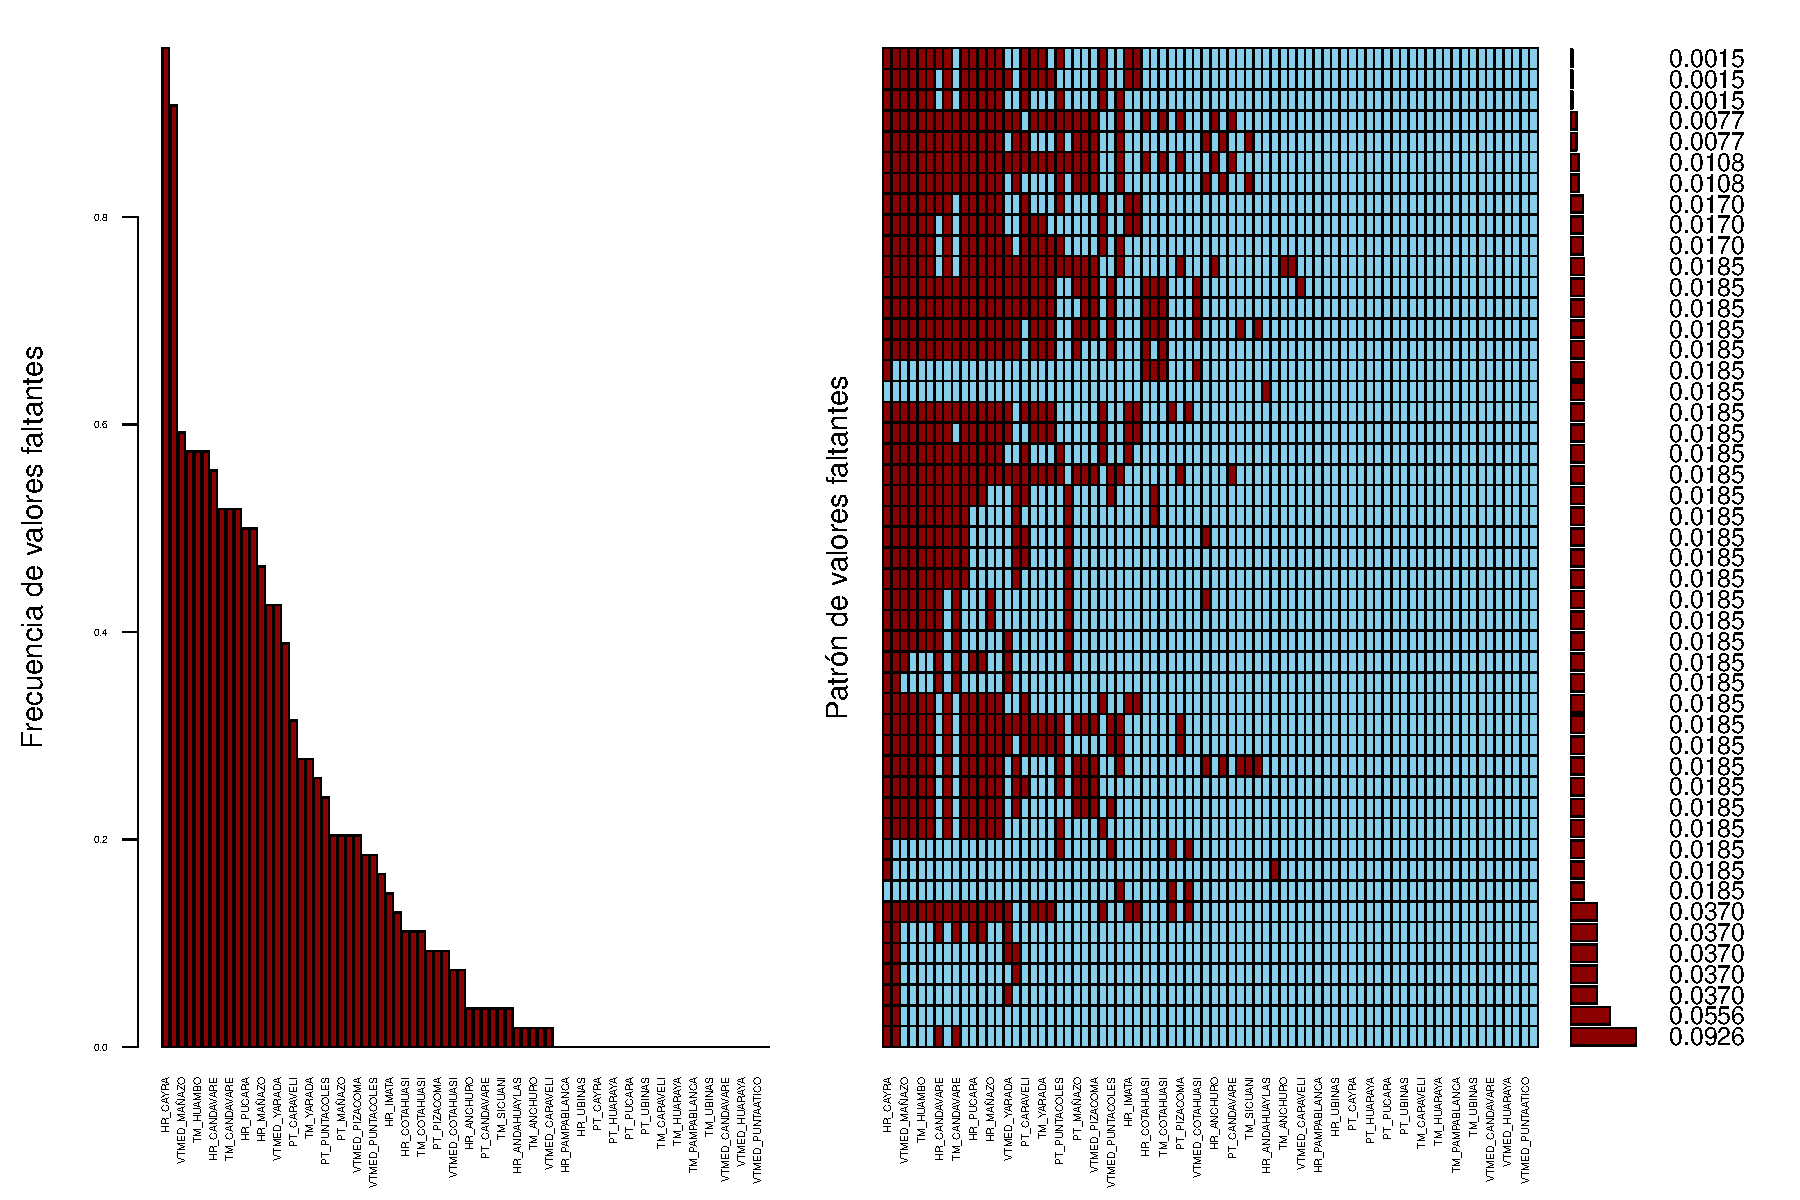
\includegraphics[width=\textwidth]{Capitulos/datos_faltanes/grafico_general.pdf} 
    
    \label{fig:valores_faltantes}
\end{figure}


En la siguiente tabla, se muestran las proporciones de valores faltantes por estación para las variables de **Humedad Relativa (HR)**, **Precipitación (PT)**, **Temperatura (TM)** y **Velocidad Media del Viento (VTMED)**, ordenadas de mayor a menor proporción de valores faltantes.

\begin{table}[H]
    \centering
    \footnotesize  % Reduce aún más el tamaño de la fuente
    \renewcommand{\arraystretch}{1.2}  % Ajusta el espacio entre filas (opcional)
    \setlength{\tabcolsep}{8pt}  % Ajusta el espacio entre las columnas
    \caption{Proporción de Valores Faltantes por Estación y Variable}
    \begin{tabular}{lcccc}
    \hline
    \textbf{Estación} & \textbf{Humedad Rel. (HR)} & \textbf{Precipitación (PT)} & \textbf{Temperatura (TM)} & \textbf{VTMED} \\
    \hline
    CAYRA       & 0.96 & 0.31 & 0.91 & 0.91 \\
    HUAMBO      & 0.57 & 0.26 & 0.59 & 0.57 \\
    CANDAVARE   & 0.56 & 0.24 & 0.57 & 0.37 \\
    CORACORA    & 0.52 & 0.20 & 0.43 & 0.04 \\
    PUCARA      & 0.50 & 0.20 & 0.20 & 0.02 \\
    MAÑAZO      & 0.46 & 0.17 & 0.19 & 0.19 \\
    PIZACOMA    & 0.39 & 0.11 & 0.19 & 0.20 \\
    YARADA      & 0.28 & 0.09 & 0.07 & 0.19 \\
    IMATA       & 0.15 & 0.04 & 0.19 & 0.19 \\
    HUARAYA     & 0.13 & 0.00 & 0.00 & 0.00 \\
    COTAHUASI   & 0.11 & 0.00 & 0.00 & 0.00 \\
    PUNTACOLES  & 0.09 & 0.00 & 0.00 & 0.00 \\
    ANCHURO     & 0.04 & 0.00 & 0.02 & 0.00 \\
    SICUANI     & 0.04 & 0.00 & 0.00 & 0.00 \\
    ANDAHUAYLAS & 0.02 & 0.00 & 0.00 & 0.00 \\
    CARAVELI    & 0.00 & 0.00 & 0.00 & 0.00 \\
    PAMPABLANCA & 0.00 & 0.00 & 0.00 & 0.00 \\
    PUNTAATICO  & 0.00 & 0.00 & 0.00 & 0.00 \\
    UBINAS      & 0.00 & 0.00 & 0.00 & 0.00 \\
    \hline
    \end{tabular}
    \label{tab:datos_faltantes}
\end{table}


\section{Imputación de Datos Faltantes Mediante MICE}

\noindent
En la presente investigación se optó por el uso del algoritmo \textbf{MICE} (\textit{Multiple Imputation by Chained Equations}, que en español se traduce como \textit{Imputación Múltiple mediante Ecuaciones Encadenadas}) para la imputación de los valores faltantes en las estaciones meteorológicas. MICE se basa en la idea de generar \textbf{m} conjuntos de datos completos (cada uno imputado de forma ligeramente diferente), lo que permite capturar la incertidumbre inherente en el proceso de imputación. Cada conjunto imputado es luego analizado de manera independiente, y los resultados se combinan para reflejar dicha variabilidad en las estimaciones finales.

\noindent
La expresión general de MICE puede verse como un procedimiento iterativo, donde cada variable con datos faltantes se modela en función de las demás variables, actualizando sucesivamente las estimaciones en cada paso. Entre cada iteración se utilizan \textit{ecuaciones encadenadas} que llenan los huecos de cada variable tomando en cuenta la información de las restantes. En el presente caso, se empleó el método \textbf{pmm} (\textit{predictive mean matching}), por ser considerado más robusto para datos climáticos; asimismo, se establecieron \texttt{m = 10} imputaciones, \texttt{maxit = 20} iteraciones para lograr convergencia, y se fijó una semilla \texttt{seed = 123} para garantizar la reproducibilidad de los resultados.

\noindent
Se decidió aplicar MICE tras comparar otras técnicas simples de imputación, como la media o la regresión lineal simple, que demostraron un ajuste menos representativo para datos estacionarios propios de las variables hidrometeorológicas. En particular, la imputación mediante ecuaciones encadenadas ofrece la ventaja de respetar la distribución original de los datos y la relación entre variables. Esto reviste especial importancia al modelar fenómenos como la sequía con modelos de dependencia (por ejemplo, cópulas), pues la calidad y completitud de los datos son determinantes para garantizar la validez de las conclusiones.

\section{Análisis de la Tendencia de las Variables Hidrometeorológicas}

El análisis de tendencias es una herramienta crucial para entender cómo evolucionan las variables climáticas a lo largo del tiempo y para predecir sus posibles efectos a largo plazo. En este estudio, se aplicó el análisis de tendencias a varias variables hidrometeorológicas provenientes de diferentes estaciones meteorológicas en el sur del Perú. Las variables consideradas incluyen la humedad relativa (\( X_1 \)), la precipitación (\( X_2 \)), la temperatura (\( X_3 \)) y la velocidad media del viento (\( X_4 \)). El principal objetivo de este análisis es identificar si alguna de estas variables presenta una tendencia significativa con el tiempo, lo que permitiría detectar patrones a largo plazo relevantes para la gestión de recursos hídricos y la planificación agrícola.

Para evaluar la tendencia de las variables hidrometeorológicas, se utilizó la regresión lineal simple, que es una técnica estadística ampliamente utilizada para modelar la relación entre una variable dependiente (\( Y \)) y una variable independiente, que en este caso es el tiempo (\( AÑO \)). La formulación del modelo de regresión lineal es la siguiente:

\[
Y = \beta_0 + \beta_1 \cdot AÑO + \epsilon
\]

Donde:
\begin{itemize}
    \item \( Y \) es la variable dependiente (\( X_1 \), \( X_2 \), \( X_3 \), \( X_4 \)).
    \item \( AÑO \) es la variable independiente que representa el tiempo.
    \item \( \beta_0 \) es el intercepto de la regresión, es decir, el valor de \( Y \) cuando \( AÑO = 0 \).
    \item \( \beta_1 \) es la pendiente de la regresión, que describe la tasa de cambio de la variable dependiente respecto al tiempo.
    \item \( \epsilon \) es el término de error, que refleja la variabilidad no explicada por el modelo.
\end{itemize}

A partir de este modelo, se puede evaluar si la variable de interés presenta una tendencia significativa a lo largo del tiempo.

\subsection{Justificación del Método de Imputación y Elección del Modelo}

Para el análisis de las series temporales, se utilizó el método \texttt{MICE} (Multiple Imputation by Chained Equations), que es particularmente útil para tratar los valores faltantes en datos climáticos. Este enfoque es ideal porque permite capturar la incertidumbre inherente a los valores ausentes y modelar las relaciones complejas entre las variables de las series temporales. Este método fue preferido sobre la imputación por media o la regresión simple, ya que estas técnicas no ofrecieron buenos resultados cuando se probaron en datos con patrones no estacionarios y fluctuaciones no lineales.

El método \texttt{MICE} proporcionó imputaciones más realistas y precisas, ajustándose mejor a la naturaleza de las fluctuaciones observadas en los datos, lo que lo convierte en la opción más adecuada para este estudio.

\subsection{Prueba de Hipótesis}

En el análisis de tendencias, se formula una prueba de hipótesis para determinar si existe una tendencia significativa en los datos. La hipótesis nula (\( H_0 \)) establece que no hay una tendencia significativa en la variable, mientras que la hipótesis alternativa (\( H_1 \)) plantea que sí existe una tendencia significativa. Las hipótesis son:

\[
H_0: \beta_1 = 0 \quad \text{(no hay tendencia significativa)}
\]
\[
H_1: \beta_1 \neq 0 \quad \text{(hay tendencia significativa)}
\]

Se utiliza el valor \( t \) obtenido de la regresión para comparar con el valor crítico \( t \), basado en una distribución \( t \) con un nivel de confianza del 95\%. Si el valor absoluto de \( t \) es mayor que el valor crítico \( t \), se rechaza la hipótesis nula y se concluye que la tendencia es significativa. Si el valor de \( t \) es menor que el valor crítico, no se rechaza la hipótesis nula, lo que indica que no hay suficiente evidencia para afirmar que existe una tendencia significativa.

\subsection{Corrección de la Tendencia}

En caso de que la prueba de hipótesis indique que la tendencia es significativa, el siguiente paso es corregir la serie temporal para eliminar la influencia de dicha tendencia. Para ello, se utiliza el valor de la tendencia ajustada, \( T_{mpt} \), que representa los valores estimados de la variable, ajustados por el modelo de regresión.


Los valores ajustados de la tendencia se obtienen utilizando la función de predicción de la regresión lineal, que se expresa como:

\[
T_{m_{p_t}} = \hat{Y} = \beta_0 + \beta_1 \cdot AÑO
\]


Donde \( \hat{Y} \) es la serie temporal ajustada que refleja la tendencia. En este caso, \( T_{\text{mpt}} \) es el valor de la tendencia calculado para cada observación en el tiempo \( AÑO \). Si la serie temporal original tiene una tendencia significativa, esta se elimina restando los valores de \( T_{\text{mpt}} \) de la serie original y ajustando los valores para reflejar solo la variabilidad intrínseca de los datos.


Una vez calculados los valores ajustados, se procede a sustituir los valores negativos (si los hubiera) por cero, dado que no tiene sentido tener valores negativos para estas variables climáticas.

Los coeficientes \( A_m \) y \( B_m \) son los valores estimados del intercepto y la pendiente de la regresión lineal, respectivamente, y se usan para ajustar los datos de acuerdo con la fórmula:

\[
Y_{\text{ajustada}} = Y - T_{\text{mpt}} + \text{media}(Y)
\]


De este modo, se genera una serie temporal "sin tendencia", en la que se eliminan los efectos de la tendencia temporal, dejando solo la variabilidad natural de los datos.

\subsection{Resumen del Procedimiento}

En resumen, el análisis de tendencias mediante regresión lineal y el uso del método \texttt{MICE} permitió realizar un análisis robusto de las variables climáticas. La identificación de tendencias significativas en varias de las estaciones meteorológicas permitió proceder con la corrección de estas tendencias, asegurando que las series temporales utilizadas en el análisis posterior reflejan únicamente la variabilidad intrínseca de los datos sin ser sesgadas por tendencias temporales que podrían alterar los resultados.

El procedimiento realizado garantiza que las series temporales analizadas son fiables y adecuadas para la realización de estudios futuros sobre las variables hidrometeorológicas.

\begin{landscape}
\begin{table}[ht]
\centering
\caption{Resumen de estaciones meteorológicas: coeficientes de determinación ($r^2$) y estadísticas $t$ para las variables HR, PT, TM y VTMED}
\begin{adjustbox}{valign=c, width=\textwidth}
\begin{tabular}{lcccccccc}
\toprule
\textbf{Estación} & \textbf{HR $r^2$} & \textbf{HR t} & \textbf{PT $r^2$} & \textbf{PT t} & \textbf{TM $r^2$} & \textbf{TM t} & \textbf{VTMED $r^2$} & \textbf{VTMED t} \\
\midrule
ANCACHURO     & 0.160 & 11.103 & 0.001 &  0.836 & 0.021 &  3.685 & 0.026 &  4.123 \\
COTAHUASI     & 0.150 & 10.662 & 0.000 & -0.206 & 0.150 & 10.662 & 0.037 & -4.993 \\
ANDAHUAYLAS   & 0.312 & 17.106 & 0.004 &  1.705 & 0.022 &  3.797 & 0.314 & -17.188 \\
CANDAVARE     & 0.012 & -2.796 & 0.001 &  0.695 & 0.000 &  0.476 & 0.020 & -3.658 \\
CARAVELI      & 0.000 & -2.961 & 0.061 &  6.465 & 0.108 &  8.823 & 0.061 &  6.465 \\
CORACORA      & 0.006 & -1.971 & 0.001 &  0.827 & 0.030 &  4.506 & 0.179 & -11.865 \\
CAYRA         & 0.025 &  4.102 & 0.000 &  0.152 & 0.025 &  4.102 & 0.203 & 12.808 \\
HUAMBO        & 0.011 & -2.661 & 0.000 &  0.520 & 0.000 &  0.602 & 0.136 & -10.103 \\
HUARAYA       & 0.000 & -0.225 & 0.000 & -1.488 & 0.000 &  1.649 & 0.263 & -15.200 \\
IMATA         & 0.016 &  3.220 & 0.000 & -0.357 & 0.034 &  4.747 & 0.016 &  3.237 \\
YARADA        & 0.087 &  7.837 & 0.000 &  0.287 & 0.000 &  1.649 & 0.022 & -3.812 \\
MANAZO        & 0.057 &  6.276 & 0.000 & -1.344 & 0.026 &  4.154 & 0.007 &  2.060 \\
PAMPABLANCA   & 0.061 & -6.493 & 0.021 & -3.702 & 0.012 &  2.846 & 0.371 & -19.529 \\
PIZACOMA      & 0.075 & -7.260 & 0.004 & -1.550 & 0.015 &  3.170 & 0.092 & -8.101 \\
PUCARA        & 0.161 & -11.138& 0.000 & -1.190 & 0.000 &  0.831 & 0.058 &  1.475 \\
PUNTAATICO    & 0.090 &  8.010 & 0.000 & -0.879 & 0.000 &  1.112 & 0.008 &  2.264 \\
PUNTACOLES    & 0.018 &  3.485 & 0.009 &  2.437 & 0.006 &  2.001 & 0.035 & -4.839 \\
SICUANI       & 0.029 &  4.404 & 0.000 &  0.393 & 0.000 & -1.205 & 0.309 & -16.990 \\
UBINAS        & 0.000 &  0.057 & 0.000 &  0.615 & 0.000 &  2.441 & 0.147 & -10.571 \\
\bottomrule
\end{tabular}
\end{adjustbox}
\end{table}
\vspace{0.2cm}  % Espacio entre la tabla y la nota
\begin{justify}
\small \textbf{\textit{Nota.}} HR = Humedad Relativa, PT = Precipitación Total, TM = Temperatura Media, VTMED = Velocidad del Viento Media. Los valores de $r^2$ indican el coeficiente de determinación y los valores t provienen del test de significancia. Análisis realizado en R.
\end{justify}

\end{landscape}



En la tabla presentada, se resumen las estaciones meteorológicas analizadas, junto con las variables correspondientes y los resultados obtenidos del análisis de tendencias. Se incluyen dos parámetros principales: el coeficiente de determinación \(r^2\) y el valor de \(t\) calculado para cada variable en cada estación.

\paragraph{Coeficiente de Determinación \(r^2\):} El coeficiente de determinación \(r^2\) refleja la proporción de la variabilidad de la variable dependiente (como la humedad relativa, la precipitación, la temperatura o la velocidad del viento) que puede ser explicada por la variable independiente (el tiempo). Cuanto mayor sea el valor de \(r^2\), mayor es la capacidad del modelo para explicar la variabilidad de la variable con respecto al tiempo. Un \(r^2\) cercano a 1 sugiere una fuerte relación entre la variable y el tiempo, mientras que valores cercanos a 0 indican que el tiempo tiene poca o ninguna influencia en la variable.

\paragraph{Valor de t Calculado:} El valor de \(t\) calculado se utiliza para evaluar la significancia estadística de la tendencia. Un valor absoluto de \(t\) mayor que el valor crítico (\(t_{crítico} = 1.964\) con un nivel de confianza del 95\%) indica que la tendencia es significativa. Esto implica que la variable presenta una relación estadísticamente significativa con el tiempo. Si el valor de \(t\) es menor que el valor crítico, no se puede concluir que exista una tendencia significativa.

\paragraph{Estaciones con Tendencias Significativas:} En las estaciones que muestran tendencias significativas, los valores de \(r^2\) y \(t\) indican que el tiempo tiene una influencia considerable en las variables analizadas. Por ejemplo, en la estación ANDAHUAYLAS la variable Humedad relativa, el coeficiente de determinación es \(r^2 = 0.312\), lo que indica una moderada capacidad de explicación del modelo. Además, el valor de \(t = 17.106\) es mucho mayor que el valor crítico de 1.964, lo que confirma que la tendencia es significativa. De manera similar, en estaciones como **TM\_COTAHUASI** y **VTMED\_YARADA**, los valores de \(t\) también superan el valor crítico, lo que sugiere que las variables presentan tendencias significativas con el tiempo.

\paragraph{Estaciones con Tendencias No Significativas:} En contraste, algunas estaciones presentan tendencias no significativas. Por ejemplo, en la estación **PT\_ANCACHURO**, el coeficiente de determinación es \(r^2 = 0.001\) y el valor de \(t = 0.836\) es inferior al valor crítico de 1.964, lo que indica que no hay suficiente evidencia para concluir que existe una tendencia significativa en la precipitación de esta estación. Otras estaciones como **PT\_COTAHUASI** y **PT\_PUNTAATICO** también presentan valores de \(r^2\) cercanos a 0 y valores de \(t\) menores que el valor crítico, lo que significa que las tendencias no son estadísticamente significativas.

\paragraph{Implicaciones de los Resultados:} Las estaciones que presentan tendencias significativas en variables clave, como la **humedad relativa** y la **temperatura media**, pueden ser cruciales para la toma de decisiones en sectores como la agricultura y la gestión de recursos hídricos. Por ejemplo, las estaciones **ANDAHUAYLAS** y **CANDAVARE** muestran tendencias significativas en la humedad relativa, lo que puede influir en la planificación de cultivos y la gestión del agua. Por otro lado, las estaciones sin tendencias significativas, como **PT\_ANCACHURO**, sugieren que la precipitación no está siendo afectada por una tendencia temporal clara en los últimos años.

En conclusión, este análisis proporciona una comprensión detallada de cómo las variables hidrometeorológicas están cambiando con el tiempo en diferentes estaciones, lo que puede ser útil para los estudios de cambio climático y la planificación de estrategias de adaptación a largo plazo.


\begin{table}[ht!]
\centering
\caption{Análisis de correlaciones climáticas por estación}
\resizebox{\textwidth}{!}{%
\begin{tabular}{lcccccl}
\toprule
\textbf{Estación} & \textbf{PT-HR} & \textbf{PT-TM} & \textbf{HR-TM} & \textbf{VTMED} & \textbf{Multicolinealidad} & \textbf{Sugerencia de Variables} \\
\midrule
Andahuaylas        & Moderada        & Moderada        & Baja            & Baja             & No                  & PT, HR, TM                   \\
Ancachuro          & Moderada        & Fuerte          & Moderada        & Baja             & Posible             & Evitar usar PT y TM juntas \\
Cayra              & Baja            & Moderada        & Muy baja        & Baja             & No                  & Priorizar TM                 \\
Sicuani            & Fuerte          & Moderada        & Baja            & Baja             & Posible             & HR clave, cuidado con PT     \\
Pucara             & Moderada        & Moderada        & Baja            & Baja             & No                  & PT, TM, HR                   \\
Manazo             & Fuerte          & Baja            & Muy baja        & Baja             & Posible             & HR clave, PT opcional        \\
Huaraya            & Moderada        & Moderada        & Baja            & Baja             & No                  & PT, HR, TM                   \\
Coracora           & Moderada        & Baja            & Moderada        & Baja             & No                  & Priorizar HR                 \\
Cotahuasi          & Fuerte          & Baja            & Baja            & Baja             & Posible             & Priorizar HR                 \\
Caravelí           & Baja            & Baja            & Baja            & Baja             & No                  & Variables independientes     \\
Huambo             & Fuerte          & Moderada        & Moderada        & Moderada         & Sí                  & Elegir una entre PT/HR y TM/VTMED \\
Candavare          & Moderada        & Moderada        & Muy fuerte      & Baja             & Alta                & Evitar usar HR y TM juntas   \\
Imata              & Fuerte          & Moderada        & Baja            & Baja             & Posible             & Priorizar HR y TM            \\
Ubinas             & Fuerte          & Baja            & Baja            & Moderada negativa & Posible             & Priorizar HR                 \\
Pizacoma           & Moderada        & Moderada        & Baja            & Baja             & No                  & HR relevante                 \\
Yarada             & Muy baja        & Baja            & Moderada negativa & Baja             & No                  & Variables independientes     \\
Pampablanca        & Baja            & Baja            & Moderada negativa & Baja             & No                  & Evaluar HR y TM (negativa)   \\
Puntaatico         & Baja            & Baja            & Moderada negativa & Baja             & No                  & Variables independientes     \\
Puntacoles         & Baja            & Baja            & Baja            & Baja             & No                  & Variables independientes     \\
\bottomrule
\end{tabular}%
}
\end{table}







  % Inicia la orientación horizontal

\begin{table}[ht]
\centering
\small
\caption{Resultados de correlaciones SPI vs variables climáticas por estación}
\resizebox{\textwidth}{!}{%
\begin{tabular}{ccccc}
\hline
\rowcolor{gray!20} \textbf{Estación} & \textbf{Pearson} & \textbf{Spearman} & \textbf{Kendall} & \textbf{Covarianza} \\
\hline
\rowcolor{gray!10} ANDAHUAYLAS & 0.33 & 0.34 & 0.23 & 2.44 \\
\rowcolor{white} ANCACHURO   & 0.46 & 0.47 & 0.32 & 4.09 \\
\rowcolor{gray!10} CAYRA       & 0.16 & 0.18 & 0.12 & 0.88 \\
\rowcolor{white} SICUANI     & 0.71 & 0.75 & 0.55 & 7.63 \\
\rowcolor{gray!10} PUCARA      & 0.41 & 0.41 & 0.28 & 4.82 \\
\rowcolor{white} MANAZO      & 0.68 & 0.70 & 0.51 & 9.43 \\
\rowcolor{gray!10} HUARAYA     & 0.44 & 0.47 & 0.33 & 4.30 \\
\rowcolor{white} CORACORA    & 0.58 & 0.61 & 0.43 & 10.29 \\
\rowcolor{gray!10} COTAHUASI   & 0.75 & 0.77 & 0.57 & 14.56 \\
\rowcolor{white} CARAVELI    & 0.35 & 0.42 & 0.28 & 5.79 \\
\rowcolor{gray!10} HUAMBO      & 0.69 & 0.71 & 0.51 & 12.51 \\
\rowcolor{white} CANDAVARE   & 0.53 & 0.60 & 0.42 & 9.19 \\
\hline
\end{tabular}%
}
\end{table}







\section{Analisis de la curva doble masa}


\begin{landscape}
\begin{table}[htbp]
\centering
\caption{Matriz de correlación de Humedad Relativa entre estaciones}
\arrayrulecolor[HTML]{006400}
\resizebox{1.4\textwidth}{!}{%
\begin{tabular}{lccccccccccccccccccc}
\toprule
\rowcolor{gray!20} % Color para las celdas del encabezado
 & ANC & COT & AND & CAN & CAR & COR & CAY & HUA & HRY & IMA & YAR & MAN & PBL & PIZ & PUC & PTA & PTC & SIC & UBI \\
\midrule
\arrayrulecolor[HTML]{006400} % Color de las líneas (verde oscuro)
\textbf{ANC}  & 1.00  & 0.46  & 0.49  & 0.35  & 0.44  & 0.24  & 0.03  & 0.26  & 0.26  & 0.36  & 0.07  & 0.41  & -0.43 & 0.14  & -0.13 & -0.19 & -0.16 & 0.33  & 0.33  \\
\textbf{COT}  & 0.46  & 1.00  & 0.33  & 0.66  & 0.63  & 0.75  & 0.19  & 0.86  & 0.43  & 0.71  & -0.30 & 0.76  & -0.32 & 0.51  & 0.38  & -0.31 & -0.04 & 0.69  & 0.82  \\
\textbf{AND}  & 0.49  & 0.33  & 1.00  & 0.18  & 0.34  & 0.17  & 0.12  & 0.19  & 0.19  & 0.35  & 0.06  & 0.38  & -0.33 & 0.20  & -0.26 & -0.05 & -0.08 & 0.38  & 0.26  \\
\textbf{CAN}  & 0.35  & 0.66  & 0.18  & 1.00  & 0.49  & 0.56  & 0.12  & 0.55  & 0.41  & 0.48  & -0.25 & 0.44  & -0.21 & 0.40  & 0.27  & -0.35 & -0.06 & 0.45  & 0.56  \\
\textbf{CAR}  & 0.44  & 0.63  & 0.34  & 0.49  & 1.00  & 0.41  & 0.11  & 0.56  & 0.40  & 0.49  & -0.14 & 0.52  & -0.29 & 0.42  & 0.12  & -0.33 & 0.01  & 0.41  & 0.57  \\
\textbf{COR}  & 0.24  & 0.75  & 0.17  & 0.56  & 0.41  & 1.00  & 0.04  & 0.69  & 0.24  & 0.57  & -0.30 & 0.52  & -0.30 & 0.41  & 0.39  & -0.30 & -0.10 & 0.60  & 0.69  \\
\textbf{CAY}  & 0.03  & 0.19  & 0.12  & 0.12  & 0.11  & 0.04  & 1.00  & 0.17  & -0.01 & 0.22  & -0.38 & 0.33  & 0.04  & 0.13  & 0.12  & -0.06 & 0.19  & 0.18  & 0.15  \\
\textbf{HUA}  & 0.26  & 0.86  & 0.19  & 0.55  & 0.56  & 0.69  & 0.17  & 1.00  & 0.45  & 0.65  & -0.32 & 0.74  & -0.24 & 0.57  & 0.46  & -0.29 & -0.05 & 0.69  & 0.81  \\
\textbf{HRY}  & 0.26  & 0.43  & 0.19  & 0.41  & 0.40  & 0.24  & -0.01 & 0.45  & 1.00  & 0.22  & 0.00  & 0.30  & -0.35 & 0.45  & 0.08  & -0.07 & -0.03 & 0.38  & 0.44  \\
\textbf{IMA}  & 0.36  & 0.71  & 0.35  & 0.48  & 0.49  & 0.57  & 0.22  & 0.65  & 0.22  & 1.00  & -0.20 & 0.70  & -0.12 & 0.49  & 0.34  & -0.21 & 0.06  & 0.60  & 0.69  \\
\textbf{YAR}  & 0.07  & -0.30 & 0.06  & -0.25 & -0.14 & -0.30 & -0.38 & -0.32 & 0.00  & -0.20 & 1.00  & -0.16 & -0.06 & -0.25 & -0.41 & 0.21  & -0.07 & -0.13 & -0.28 \\
\textbf{MAN}  & 0.41  & 0.76  & 0.38  & 0.44  & 0.52  & 0.52  & 0.33  & 0.74  & 0.30  & 0.70  & -0.16 & 1.00  & -0.21 & 0.39  & 0.32  & -0.17 & 0.03  & 0.74  & 0.70  \\
\textbf{PBL}  & -0.43 & -0.32 & -0.33 & -0.21 & -0.29 & -0.30 & 0.04  & -0.24 & -0.35 & -0.12 & -0.06 & -0.21 & 1.00  & -0.11 & -0.11 & 0.21  & 0.10  & -0.28 & -0.34 \\
\textbf{PIZ}  & 0.14  & 0.51  & 0.20  & 0.40  & 0.42  & 0.41  & 0.13  & 0.57  & 0.45  & 0.49  & -0.25 & 0.39  & -0.11 & 1.00  & 0.27  & -0.23 & -0.13 & 0.36  & 0.56  \\
\textbf{PUC}  & -0.13 & 0.38  & -0.26 & 0.27  & 0.12  & 0.39  & 0.12  & 0.46  & 0.08  & 0.34  & -0.41 & 0.32  & 0.11  & 0.27  & 1.00  & -0.23 & -0.06 & 0.10  & 0.39  \\
\textbf{PTA}  & -0.19 & -0.31 & -0.05 & -0.35 & -0.33 & -0.30 & -0.06 & -0.29 & -0.07 & -0.21 & 0.21  & -0.17 & 0.21  & -0.23 & -0.23 & 1.00  & 0.16  & -0.21 & -0.34 \\
\textbf{PTC}  & -0.16 & -0.04 & -0.08 & -0.06 & 0.01  & -0.10 & 0.19  & -0.05 & -0.03 & 0.06  & -0.07 & 0.03  & 0.10  & -0.13 & 0.10  & 1.00  & -0.08 & -0.02 & -0.02 \\
\textbf{SIC}  & 0.33  & 0.69  & 0.38  & 0.45  & 0.41  & 0.60  & 0.18  & 0.69  & 0.38  & 0.60  & -0.13 & 0.74  & -0.28 & 0.36  & 0.23  & -0.21 & -0.08 & 1.00  & 0.70  \\
\textbf{UBI}  & 0.33  & 0.82  & 0.26  & 0.56  & 0.57  & 0.69  & 0.15  & 0.81  & 0.44  & 0.69  & -0.28 & 0.70  & -0.34 & 0.56  & 0.39  & -0.34 & -0.02 & 0.70  & 1.00  \\
\hline
\end{tabular}
}
\vspace{0.5em}
\begin{flushleft}
\footnotesize
\textbf{\textit{Nota}}: ANC = Ancachuro, COT = Cotahuasi, AND = Andahuaylas, CAN = Candavare, CAR = Caravelí, COR = Coracora, CAY = Cayra, HUA = Huambo, HRY = Huaraya, IMA = Imata, YAR = Yarada, MAN = Mañazo, PBL = Pampablanca, PIZ = Pizacoma, PUC = Pucará, PTA = Punta Atico, PTC = Punta Coles, SIC = Sicuani, UBI = Ubinas.
\end{flushleft}
\end{table}
\end{landscape}



\begin{landscape}
\begin{table}[htbp]
\centering
\caption{Matriz de correlación de temperatura media entre estaciones}
\arrayrulecolor[HTML]{006400}
\resizebox{1.4\textwidth}{!}{%
\begin{tabular}{lccccccccccccccccccc}
\toprule
\rowcolor{gray!20} % Color para las celdas del encabezado
 & ANC & COT & AND & CAN & CAR & COR & CAY & HUA & HRY & IMA & YAR & MAN & PBL & PIZ & PUC & PTA & PTC & SIC & UBI \\
\midrule
\arrayrulecolor[HTML]{006400} % Color de las líneas (verde oscuro)
\textbf{ANC}  & 1.00  & 0.51  & 0.83  & 0.63  & 0.70  & 0.69  & 0.83  & 0.69  & 0.83  & 0.88  & 0.63  & 0.75  & 0.69  & 0.84  & 0.81  & 0.60  & 0.64  & 0.79  & 0.81  \\
\textbf{COT}  & 0.51  & 1.00  & 0.68  & 0.56  & 0.74  & 0.69  & 0.65  & 0.58  & 0.62  & 0.55  & 0.22  & 0.69  & 0.24  & 0.60  & 0.54  & 0.19  & 0.26  & 0.56  & 0.66  \\
\textbf{AND}  & 0.83  & 0.68  & 1.00  & 0.76  & 0.76  & 0.79  & 0.90  & 0.69  & 0.88  & 0.86  & 0.55  & 0.85  & 0.60  & 0.88  & 0.85  & 0.52  & 0.57  & 0.85  & 0.87  \\
\textbf{CAN}  & 0.63  & 0.56  & 0.76  & 1.00  & 0.62  & 0.76  & 0.69  & 0.59  & 0.73  & 0.69  & 0.41  & 0.65  & 0.43  & 0.75  & 0.66  & 0.37  & 0.44  & 0.70  & 0.72  \\
\textbf{CAR}  & 0.70  & 0.74  & 0.76  & 0.62  & 1.00  & 0.74  & 0.78  & 0.73  & 0.74  & 0.76  & 0.48  & 0.70  & 0.54  & 0.75  & 0.70  & 0.47  & 0.52  & 0.67  & 0.77  \\
\textbf{COR}  & 0.69  & 0.69  & 0.79  & 0.76  & 0.74  & 1.00  & 0.76  & 0.67  & 0.73  & 0.74  & 0.39  & 0.70  & 0.41  & 0.75  & 0.69  & 0.32  & 0.40  & 0.75  & 0.81  \\
\textbf{CAY}  & 0.83  & 0.65  & 0.90  & 0.69  & 0.78  & 0.76  & 1.00  & 0.72  & 0.89  & 0.86  & 0.50  & 0.85  & 0.56  & 0.87  & 0.85  & 0.47  & 0.53  & 0.86  & 0.87  \\
\textbf{HUA}  & 0.69  & 0.58  & 0.69  & 0.59  & 0.73  & 0.67  & 0.72  & 1.00  & 0.71  & 0.76  & 0.50  & 0.63  & 0.56  & 0.68  & 0.73  & 0.51  & 0.54  & 0.69  & 0.76  \\
\textbf{HRY}  & 0.83  & 0.62  & 0.88  & 0.73  & 0.74  & 0.73  & 0.89  & 0.71  & 1.00  & 0.86  & 0.57  & 0.87  & 0.61  & 0.89  & 0.88  & 0.59  & 0.54  & 0.88  & 0.84  \\
\textbf{IMA}  & 0.88  & 0.55  & 0.86  & 0.69  & 0.76  & 0.74  & 0.86  & 0.76  & 0.86  & 1.00  & 0.72  & 0.78  & 0.77  & 0.90  & 0.87  & 0.69  & 0.73  & 0.79  & 0.88  \\
\textbf{YAR}  & 0.63  & 0.22  & 0.55  & 0.41  & 0.48  & 0.39  & 0.50  & 0.50  & 0.57  & 0.72  & 1.00  & 0.37  & 0.95  & 0.64  & 0.63  & 0.94  & 0.94  & 0.44  & 0.54  \\
\textbf{MAN}  & 0.75  & 0.69  & 0.85  & 0.65  & 0.70  & 0.70  & 0.85  & 0.63  & 0.87  & 0.78  & 0.37  & 1.00  & 0.44  & 0.83  & 0.82  & 0.36  & 0.42  & 0.78  & 0.81  \\
\textbf{PBL}  & 0.69  & 0.24  & 0.60  & 0.43  & 0.54  & 0.41  & 0.56  & 0.56  & 0.61  & 0.77  & 0.95  & 0.44  & 1.00  & 0.69  & 0.67  & 0.97  & 0.97  & 0.47  & 0.58  \\
\textbf{PIZ}  & 0.84  & 0.60  & 0.88  & 0.75  & 0.75  & 0.75  & 0.87  & 0.68  & 0.89  & 0.90  & 0.64  & 0.83  & 0.69  & 1.00  & 0.87  & 0.60  & 0.66  & 0.81  & 0.88  \\
\textbf{PUC}  & 0.81  & 0.54  & 0.86  & 0.66  & 0.70  & 0.69  & 0.85  & 0.73  & 0.88  & 0.87  & 0.63  & 0.82  & 0.67  & 0.87  & 1.00  & 0.61  & 0.63  & 0.83  & 0.84  \\
\textbf{PTA}  & 0.60  & 0.19  & 0.52  & 0.37  & 0.47  & 0.32  & 0.47  & 0.51  & 0.54  & 0.69  & 0.94  & 0.42  & 0.97  & 0.60  & 0.61  & 1.00  & 0.96  & 0.39  & 0.50  \\
\textbf{PTC}  & 0.64  & 0.26  & 0.57  & 0.44  & 0.52  & 0.40  & 0.53  & 0.54  & 0.59  & 0.73  & 0.94  & 0.42  & 0.97  & 0.66  & 0.63  & 0.96  & 1.00  & 0.44  & 0.56  \\
\textbf{SIC}  & 0.79  & 0.56  & 0.85  & 0.70  & 0.67  & 0.75  & 0.86  & 0.69  & 0.88  & 0.79  & 0.44  & 0.78  & 0.47  & 0.81  & 0.83  & 0.44  & 0.39  & 1.00  & 0.81  \\
\textbf{UBI}  & 0.81  & 0.66  & 0.87  & 0.72  & 0.77  & 0.81  & 0.87  & 0.76  & 0.84  & 0.88  & 0.54  & 0.81  & 0.58  & 0.88  & 0.84  & 0.50  & 0.56  & 0.81  & 1.00  \\
\hline
\end{tabular}
}
\vspace{0.5em}
\begin{flushleft}
\footnotesize
\textbf{\textit{Nota}}: ANC = Ancachuro, COT = Cotahuasi, AND = Andahuaylas, CAN = Candavare, CAR = Caravelí, COR = Coracora, CAY = Cayra, HUA = Huambo, HRY = Huaraya, IMA = Imata, YAR = Yarada, MAN = Mañazo, PBL = Pampablanca, PIZ = Pizacoma, PUC = Pucará, PTA = Punta Atico, PTC = Punta Coles, SIC = Sicuani, UBI = Ubinas.
\end{flushleft}
\end{table}
\end{landscape}


\begin{landscape}
\begin{table}[htbp]
\centering
\caption{Matriz de correlación de precipitación entre estaciones}
\arrayrulecolor[HTML]{006400}
\resizebox{1.4\textwidth}{!}{%
\begin{tabular}{lccccccccccccccccccc}
\toprule
\rowcolor{gray!20} % Color para las celdas del encabezado
 & ANC & COT & AND & CAN & CAR & COR & CAY & HUA & HRY & IMA & YAR & MAN & PBL & PIZ & PUC & PTA & PTC & SIC & UBI \\
\midrule
\arrayrulecolor[HTML]{006400} % Color de las líneas (verde oscuro)
\textbf{ANC}  & 1.00  & 0.62  & 0.78  & 0.59  & 0.30  & 0.60  & 0.91  & 0.63  & 0.78  & 0.76  & -0.10 & 0.77  & 0.08  & 0.73  & 0.81  & 0.14  & -0.10 & 0.87  & 0.65  \\
\textbf{COT}  & 0.62  & 1.00  & 0.71  & 0.77  & 0.47  & 0.83  & 0.62  & 0.88  & 0.63  & 0.81  & -0.03 & 0.74  & 0.11  & 0.68  & 0.64  & 0.09  & -0.05 & 0.69  & 0.85  \\
\textbf{AND}  & 0.78  & 0.71  & 1.00  & 0.67  & 0.40  & 0.72  & 0.78  & 0.73  & 0.70  & 0.79  & -0.05 & 0.79  & 0.09  & 0.69  & 0.75  & 0.13  & -0.07 & 0.83  & 0.74  \\
\textbf{CAN}  & 0.59  & 0.77  & 0.67  & 1.00  & 0.55  & 0.79  & 0.61  & 0.81  & 0.61  & 0.80  & 0.06  & 0.70  & 0.16  & 0.70  & 0.61  & 0.10  & 0.01  & 0.63  & 0.87  \\
\textbf{CAR}  & 0.30  & 0.47  & 0.40  & 0.55  & 1.00  & 0.53  & 0.32  & 0.52  & 0.29  & 0.42  & 0.09  & 0.33  & 0.07  & 0.30  & 0.30  & 0.02  & 0.03  & 0.34  & 0.49  \\
\textbf{COR}  & 0.60  & 0.83  & 0.72  & 0.79  & 0.53  & 1.00  & 0.62  & 0.83  & 0.58  & 0.80  & -0.02 & 0.69  & 0.07  & 0.66  & 0.61  & 0.11  & -0.06 & 0.67  & 0.83  \\
\textbf{CAY}  & 0.91  & 0.62  & 0.78  & 0.61  & 0.32  & 0.62  & 1.00  & 0.62  & 0.81  & 0.78  & -0.12 & 0.81  & 0.05  & 0.78  & 0.85  & 0.15  & -0.10 & 0.88  & 0.68  \\
\textbf{HUA}  & 0.63  & 0.88  & 0.73  & 0.81  & 0.52  & 0.83  & 0.62  & 1.00  & 0.63  & 0.84  & 0.00  & 0.75  & 0.10  & 0.72  & 0.73  & 0.11  & -0.04 & 0.66  & 0.89  \\
\textbf{HRY}  & 0.78  & 0.63  & 0.70  & 0.61  & 0.29  & 0.58  & 0.81  & 0.63  & 1.00  & 0.80  & -0.07 & 0.84  & 0.09  & 0.83  & 0.88  & 0.10  & -0.08 & 0.81  & 0.71  \\
\textbf{IMA}  & 0.76  & 0.81  & 0.79  & 0.80  & 0.42  & 0.80  & 0.78  & 0.84  & 0.80  & 1.00  & -0.02 & 0.86  & 0.12  & 0.85  & 0.79  & 0.15  & -0.06 & 0.79  & 0.89  \\
\textbf{YAR}  & -0.10 & -0.03 & -0.05 & 0.06  & 0.09  & -0.02 & -0.12 & 0.00  & -0.07 & -0.02 & 1.00  & -0.08 & 0.28  & -0.03 & -0.08 & 0.02  & 0.13  & 0.13  & 0.03  \\
\textbf{MAN}  & 0.77  & 0.74  & 0.79  & 0.70  & 0.33  & 0.69  & 0.81  & 0.75  & 0.84  & 0.86  & -0.08 & 1.00  & 0.10  & 0.87  & 0.85  & 0.18  & -0.06 & 0.84  & 0.78  \\
\textbf{PBL}  & 0.08  & 0.11  & 0.09  & 0.16  & 0.07  & 0.07  & 0.05  & 0.10  & 0.09  & 0.12  & 0.28  & 0.10  & 1.00  & 0.10  & 0.06  & 0.23  & 0.18  & 0.07  & 0.13  \\
\textbf{PIZ}  & 0.73  & 0.68  & 0.69  & 0.70  & 0.75  & 0.75  & 0.87  & 0.72  & 0.83  & 0.90  & 0.64  & 0.83  & 0.69  & 1.00  & 0.79  & 0.18  & -0.06 & 0.76  & 0.78  \\
\textbf{PUC}  & 0.81  & 0.64  & 0.75  & 0.61  & 0.70  & 0.69  & 0.85  & 0.73  & 0.88  & 0.87  & 0.63  & 0.82  & 0.67  & 0.87  & 1.00  & 0.15  & -0.06 & 0.79  & 0.69  \\
\textbf{PTA}  & 0.14  & 0.09  & 0.13  & 0.10  & 0.02  & 0.11  & 0.15  & 0.11  & 0.10  & 0.15  & 0.02  & 0.18  & 0.06  & 0.18  & 0.15  & 1.00  & 0.32  & 0.16  & 0.10  \\
\textbf{PTC}  & -0.10 & -0.05 & -0.07 & 0.01  & 0.03  & -0.06 & -0.10 & -0.04 & -0.08 & -0.06 & 0.13  & -0.06 & 0.18  & -0.06 & -0.06 & 0.32  & 1.00  & -0.09 & -0.03  \\
\textbf{SIC}  & 0.87  & 0.69  & 0.83  & 0.63  & 0.34  & 0.67  & 0.88  & 0.66  & 0.81  & 0.79  & 0.44  & 0.78  & 0.47  & 0.76  & 0.79  & 0.07  & -0.09 & 1.00  & 0.70  \\
\textbf{UBI}  & 0.65  & 0.85  & 0.74  & 0.87  & 0.49  & 0.83  & 0.68  & 0.89  & 0.71  & 0.88  & 0.03  & 0.78  & 0.13  & 0.78  & 0.69  & 0.10  & -0.03 & 0.70  & 1.00  \\
\hline
\end{tabular}
}
\vspace{0.5em}
\begin{flushleft}
\footnotesize
\textbf{\textit{Nota}}: ANC = Ancachuro, COT = Cotahuasi, AND = Andahuaylas, CAN = Candavare, CAR = Caravelí, COR = Coracora, CAY = Cayra, HUA = Huambo, HRY = Huaraya, IMA = Imata, YAR = Yarada, MAN = Mañazo, PBL = Pampablanca, PIZ = Pizacoma, PUC = Pucará, PTA = Punta Atico, PTC = Punta Coles, SIC = Sicuani, UBI = Ubinas.
\end{flushleft}
\end{table}
\end{landscape}

\begin{landscape}
\begin{table}[htbp]
\centering
\caption{Matriz de correlación de velocidad media del viento entre estaciones}
\resizebox{1.4\textwidth}{!}{%
\begin{tabular}{lccccccccccccccccccc}
\toprule
\rowcolor{gray!20} % Color para las celdas del encabezado
 & \textbf{ANC} & \textbf{COT} & \textbf{AND} & \textbf{CAN} & \textbf{CAR} & \textbf{COR} & \textbf{CAY} & \textbf{HUA} & \textbf{HRY} & \textbf{IMA} & \textbf{YAR} & \textbf{MAN} & \textbf{PBL} & \textbf{PIZ} & \textbf{PUC} & \textbf{PTA} & \textbf{PTC} & \textbf{SIC} & \textbf{UBI} \\
\midrule
\arrayrulecolor[HTML]{006400} % Color de las líneas (verde oscuro)
\textbf{ANC} & 1.00  & 0.13  & -0.07 & -0.02 & 0.21 & 0.01 & 0.31 & -0.03 & -0.02 & -0.08 & -0.01 & -0.33 & -0.14 & -0.14 & 0.33 & 0.12 & 0.00  & 0.12 & 0.06 \\
\textbf{COT} & 0.13  & 1.00  & 0.28  & 0.40  & -0.04 & 0.52 & 0.03 & 0.14  & 0.23 & 0.25 & 0.04 & 0.40 & 0.03 & 0.16 & -0.23 & 0.28 & 0.06  & 0.47 & 0.03 \\
\textbf{AND} & -0.07 & 0.28  & 1.00  & 0.18  & -0.17 & 0.35 & -0.14 & 0.26 & 0.39 & 0.20 & 0.06 & 0.25 & 0.28 & 0.22 & -0.36 & -0.02 & 0.03  & 0.46 & 0.25 \\
\textbf{CAN} & -0.02 & 0.40  & 0.18  & 1.00  & -0.04 & 0.43 & -0.02 & 0.12 & 0.16 & 0.40 & 0.23 & 0.34 & 0.34 & 0.12 & -0.25 & 0.31 & 0.22  & 0.72 & 0.34 \\
\textbf{CAR} & 0.21  & -0.04 & -0.17 & -0.04 & 1.00  & -0.06 & 0.17  & -0.27 & -0.08 & 0.00  & 0.09 & -0.06 & -0.01 & -0.20 & 0.16  & 0.13  & -0.03 & -0.04 & -0.04 \\
\textbf{COR} & 0.01  & 0.52  & 0.35  & 0.43  & -0.06 & 1.00  & -0.14 & 0.22  & 0.26 & 0.01  & 0.22 & 0.24  & 0.47 & 0.12 & -0.18 & -0.03 & 0.29  & 0.26 & 0.11 \\
\textbf{CAY} & 0.31  & 0.03  & -0.14 & -0.02 & 0.17  & -0.14 & 1.00  & -0.06 & 0.04  & 0.22  & -0.05 & 0.17  & 0.23  & 0.43 & 0.16  & -0.02 & -0.03 & 0.38  & 0.34 \\
\textbf{HUA} & -0.03 & 0.14  & 0.26  & 0.12  & -0.27 & 0.22  & -0.06 & 1.00  & 0.21  & 0.17  & -0.15 & 0.04  & 0.23  & 0.43 & -0.27 & 0.13  & -0.25 & 0.66  & 0.50 \\
\textbf{HRY} & -0.02 & 0.23  & 0.39  & 0.16  & -0.08 & 0.26  & 0.04  & 0.21  & 1.00  & 0.10  & 0.15  & 0.11  & 0.27  & 0.21  & -0.03 & -0.03 & 0.03  & 0.10  & 0.34 \\
\textbf{IMA} & -0.08 & 0.25  & 0.20  & 0.40  & 0.00  & 0.01  & 0.22  & 0.17  & 0.10  & 1.00  & -0.02 & 0.54  & -0.11 & 0.15  & -0.22 & 0.10  & -0.06 & 0.02  & -0.02 \\
\textbf{YAR} & -0.01 & 0.04  & 0.06  & 0.23  & 0.09  & 0.22  & -0.05 & 0.15  & 0.15  & -0.04 & 1.00  & 0.05  & 0.19  & 0.10  & -0.08 & 0.12  & -0.01 & 0.34  & 0.19 \\
\textbf{MAN} & -0.33 & 0.40  & 0.25  & 0.34  & -0.06 & 0.24  & 0.17  & 0.04  & 0.11  & 0.54  & 0.05  & 1.00  & 0.10  & 0.29  & -0.37 & 0.10  & -0.09 & 0.21  & 0.05 \\
\textbf{PBL} & -0.14 & 0.03  & 0.28  & 0.34  & -0.01 & 0.47  & -0.30 & 0.23  & 0.27  & -0.11 & 0.28  & -0.09 & 1.00  & 0.07  & 0.19  & -0.03 & 0.14  & 0.07  & 0.07 \\
\textbf{PIZ} & -0.14 & 0.16  & 0.22  & 0.05  & -0.20 & 0.12  & 0.03  & 0.43  & 0.21  & 0.15  & -0.22 & 0.29  & 0.07  & 1.00  & 0.79  & 0.18  & -0.06 & 0.07  & 0.26 \\
\textbf{PUC} & 0.33  & -0.23 & -0.36 & -0.25 & 0.16  & -0.18 & 0.14  & -0.02 & -0.03 & -0.22 & 0.10  & -0.37 & -0.03 & 0.79  & 1.00  & 0.15  & -0.06 & -0.12 & -0.08 \\
\textbf{PTA} & 0.12  & 0.28  & -0.02 & 0.31  & 0.13  & 0.29  & 0.03  & 0.13  & 0.03  & 0.10  & 0.12  & 0.10  & 0.14  & 0.18  & 0.15  & 1.00  & 0.32  & 0.10  & 0.03 \\
\textbf{PTC} & 0.00  & 0.06  & 0.03  & 0.22  & -0.03 & -0.03 & -0.10 & -0.25 & 0.10  & -0.01 & -0.01 & -0.09 & 0.07  & -0.06 & -0.06 & 0.32  & 1.00  & 0.12  & -0.03 \\
\textbf{SIC} & 0.12  & 0.47  & 0.46  & 0.72  & 0.26  & 0.72  & 0.38  & 0.66  & 0.38  & 0.02  & 0.34  & 0.21  & 0.51  & 0.43  & 0.79  & 0.23  & 0.12  & 1.00  & 0.19 \\
\textbf{UBI} & 0.06  & 0.03  & 0.25  & 0.34  & -0.04 & 0.11  & 0.13  & 0.50  & 0.34  & -0.02 & 0.19  & 0.05  & 0.25  & 0.26  & 0.69  & 0.07  & -0.03 & 0.12  & 1.00  \\
\hline
\end{tabular}
}
\vspace{0.5em}
\begin{flushleft}
\footnotesize
\textbf{\textit{Nota}}: ANC = Ancachuro, COT = Cotahuasi, AND = Andahuaylas, CAN = Candavare, CAR = Caravelí, COR = Coracora, CAY = Cayra, HUA = Huambo, HRY = Huaraya, IMA = Imata, YAR = Yarada, MAN = Mañazo, PBL = Pampablanca, PIZ = Pizacoma, PUC = Pucará, PTA = Punta Atico, PTC = Punta Coles, SIC = Sicuani, UBI = Ubinas.
\end{flushleft}
\end{table}
\end{landscape}


\section{Analisis de Curva de doble masa}




\section{Calculo del SPI}


El Índice Estándar de Precipitación (SPI, por sus siglas en inglés) es una herramienta estadística utilizada para medir las variaciones en la precipitación en un determinado período de tiempo, y es ampliamente utilizado para detectar condiciones de sequía o exceso de precipitación. En este estudio, el SPI se calcula a partir de los datos históricos de precipitación de varias estaciones meteorológicas en un rango temporal específico (3, 6 y 12 meses).

\subsection{Método de Cálculo}

El cálculo del SPI se realizó utilizando la función \texttt{spi()} del paquete \texttt{SPEI} en R. Este índice se calcula con base en la distribución de los datos históricos de precipitación para cada estación y periodo de tiempo, utilizando una distribución gamma ajustada a los datos de precipitación.

El cálculo se realizó para tres períodos de tiempo diferentes: 3, 6 y 12 meses, con el objetivo de evaluar la variabilidad de la precipitación en distintos horizontes temporales. Para cada estación, se obtuvieron los valores ajustados del SPI, también conocidos como los \textit{valores \texttt{fitted}}, que son aquellos que reflejan las condiciones de precipitación estándar de acuerdo con la escala SPI.

\subsection{Tratamiento de Valores -Inf}

Durante el cálculo del SPI, se presentaron algunos valores de **-Inf**. Estos valores corresponden a situaciones donde la precipitación fue extremadamente baja o nula durante un largo período, lo que hace imposible calcular un valor válido del SPI a partir de los datos disponibles. En términos de la clasificación del SPI, valores **-Inf** indican una **sequía extremadamente seca**, es decir, que no se produjo precipitación suficiente para calcular el índice de forma estándar.

Según la escala de clasificación del SPI, los valores inferiores a **-2.0** indican condiciones de sequía extremadamente seca. Dado que los valores **-Inf** no pueden ser representados directamente, se optó por reemplazarlos por el valor **-2.0**, el cual corresponde a la categoría de sequía extrema en la escala estándar del SPI. Este tratamiento es necesario para mantener la integridad de los datos y permitir una interpretación coherente dentro del análisis global, sin perder la información crítica sobre eventos de sequía severa.

\subsection{Justificación del Tratamiento de -Inf}

La decisión de reemplazar los valores **-Inf** por **-2.0** está basada en la clasificación estándar del SPI, que define que cualquier valor igual o inferior a **-2.0** indica condiciones de sequía extrema. Este enfoque garantiza que la interpretación de los datos sea consistente y acorde con la clasificación oficial, sin perder la importancia del evento climático. Al utilizar **-2.0**, los valores de sequía extrema se manejan correctamente, asegurando que los resultados del análisis no se vean distorsionados y se mantenga la fiabilidad del indicador en el contexto de sequías prolongadas o extremas.

Este tratamiento de los valores **-Inf** asegura que los datos sean analizados de manera precisa, reflejando adecuadamente las condiciones extremas de precipitación, y manteniendo la escalabilidad y comparabilidad de los resultados dentro del análisis del SPI.


% Página 1
\begin{landscape}  % Usar orientación horizontal

\begin{figure}[h!]
\centering
% Primera fila de gráficas
\begin{minipage}{0.45\textwidth}
    \centering
    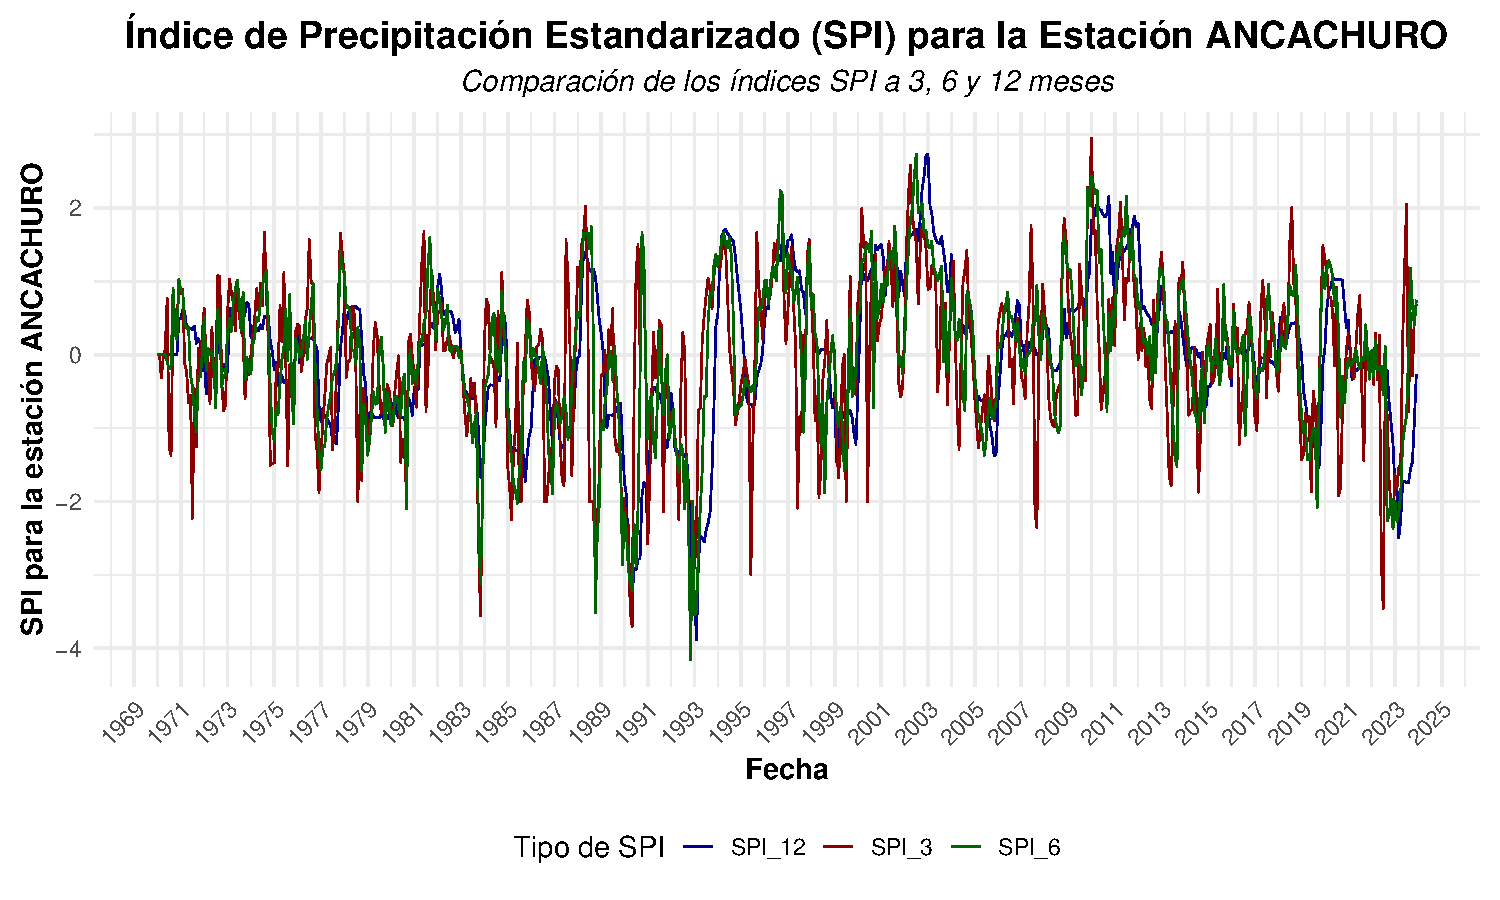
\includegraphics[width=\linewidth]{Capitulos/spi/SPI_Station_ANCACHURO.pdf}
    
\end{minipage} \hfill
\begin{minipage}{0.45\textwidth}
    \centering
    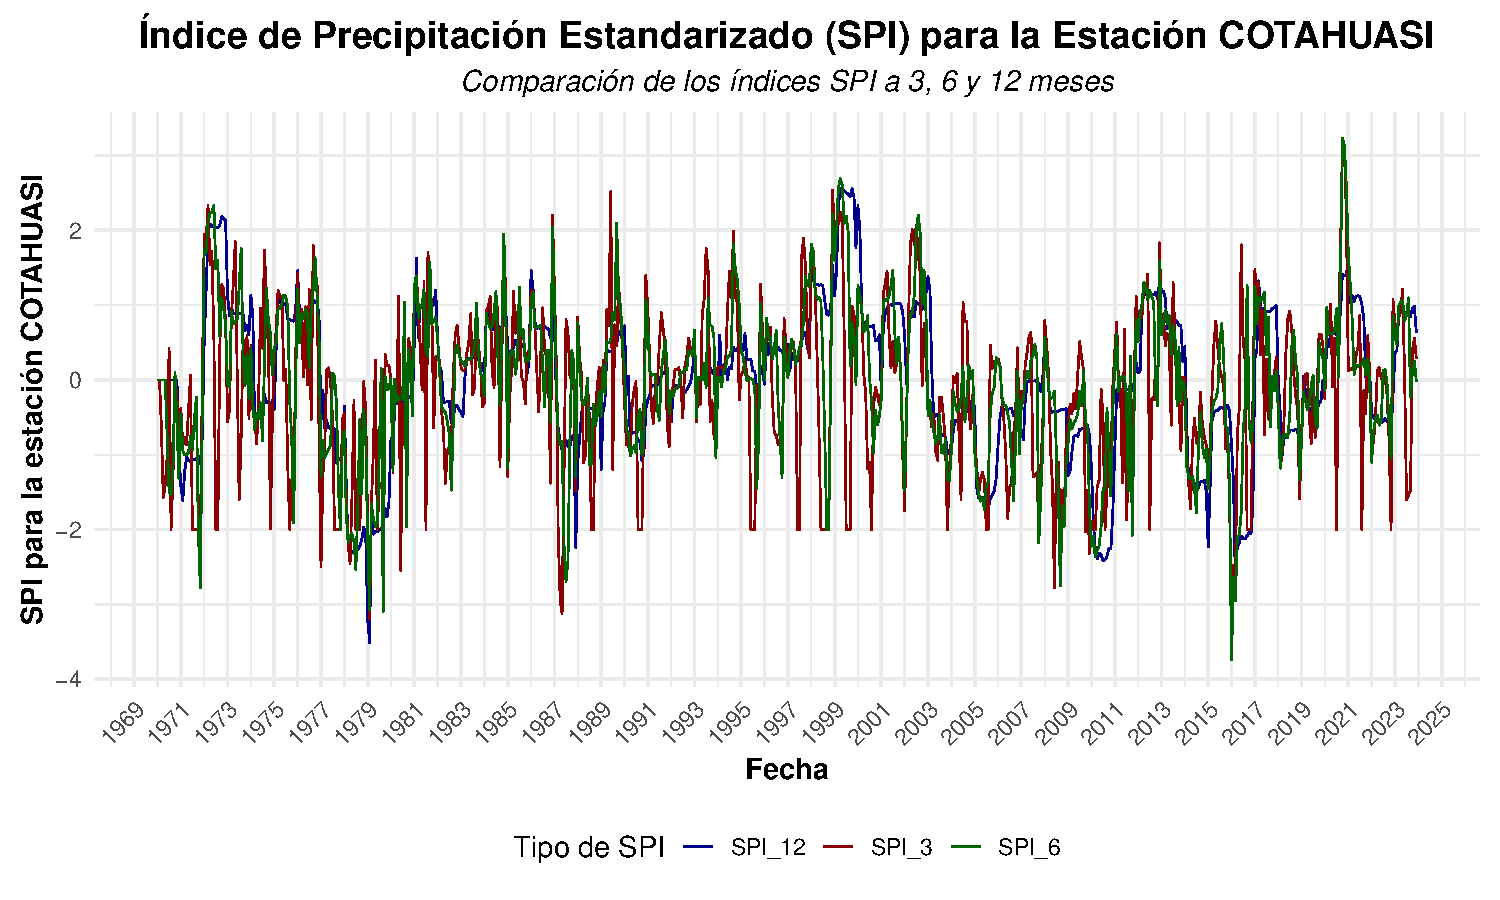
\includegraphics[width=\linewidth]{Capitulos/spi/SPI_Station_COTAHUASI.pdf}
   
\end{minipage} \hfill
\begin{minipage}{0.45\textwidth}
    \centering
    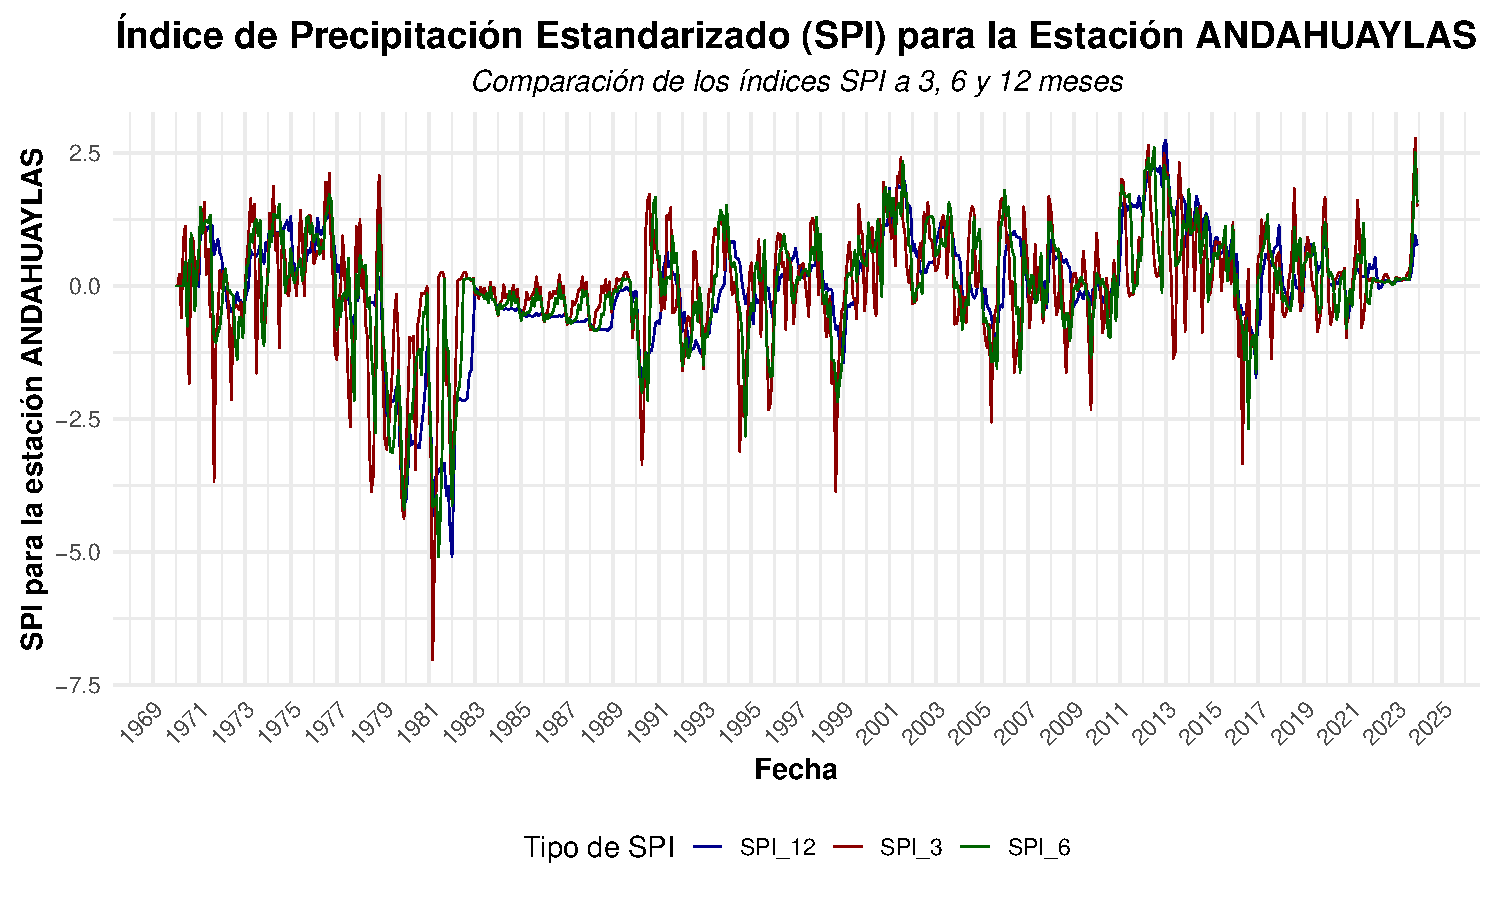
\includegraphics[width=\linewidth]{Capitulos/spi/SPI_Station_ANDAHUAYLAS.pdf}
  
\end{minipage}

\vskip\baselineskip  % Espacio entre filas de subgráficas

% Segunda fila de gráficas
\begin{minipage}{0.45\textwidth}
    \centering
    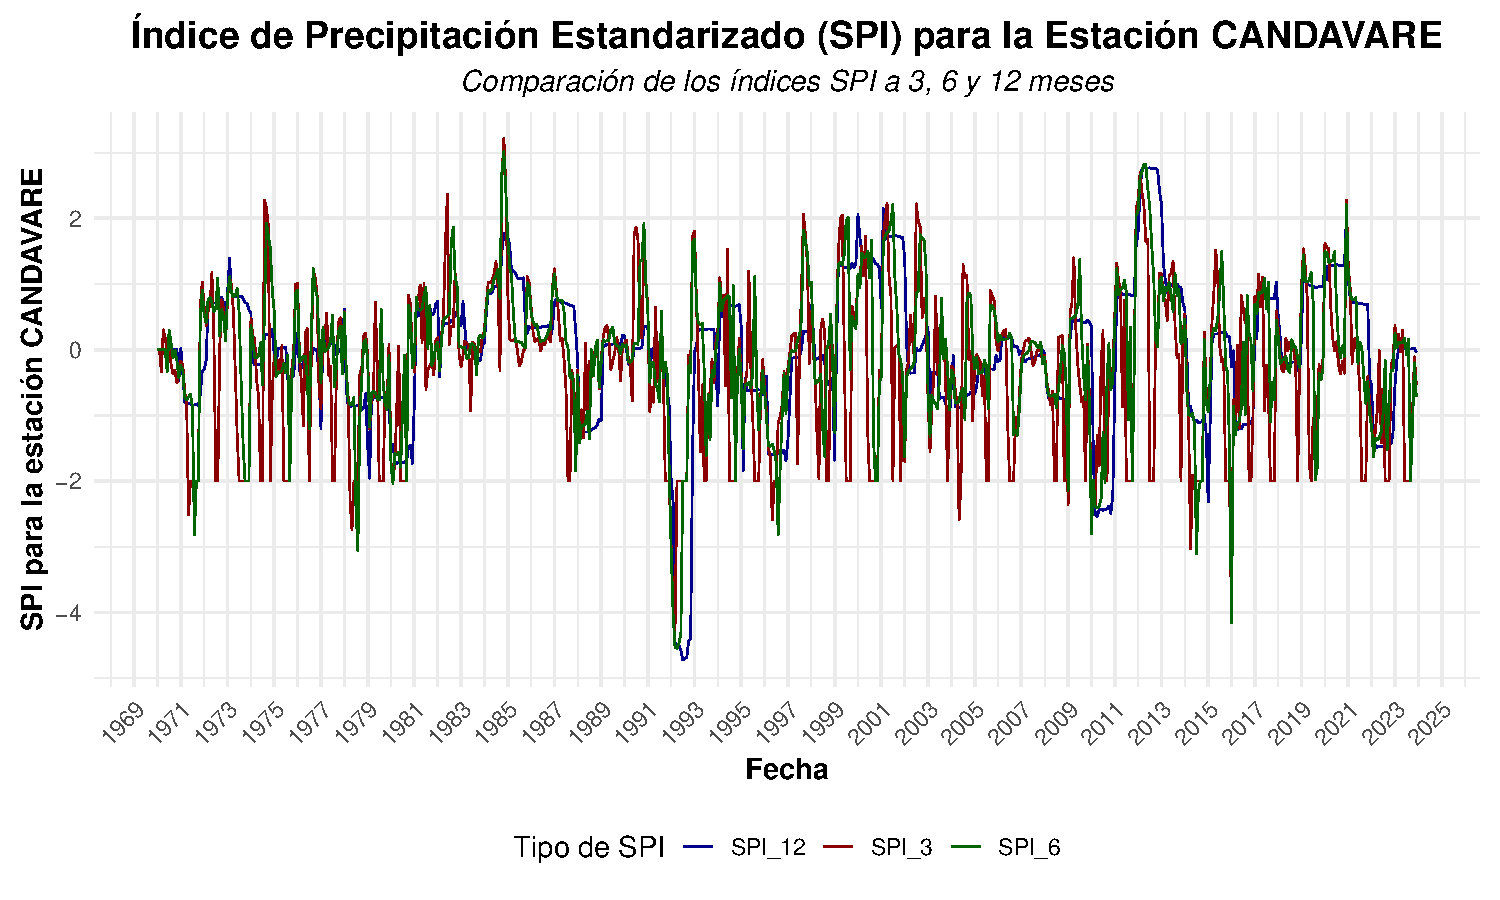
\includegraphics[width=\linewidth]{Capitulos/spi/SPI_Station_CANDAVARE.pdf}
   
\end{minipage} \hfill
\begin{minipage}{0.45\textwidth}
    \centering
    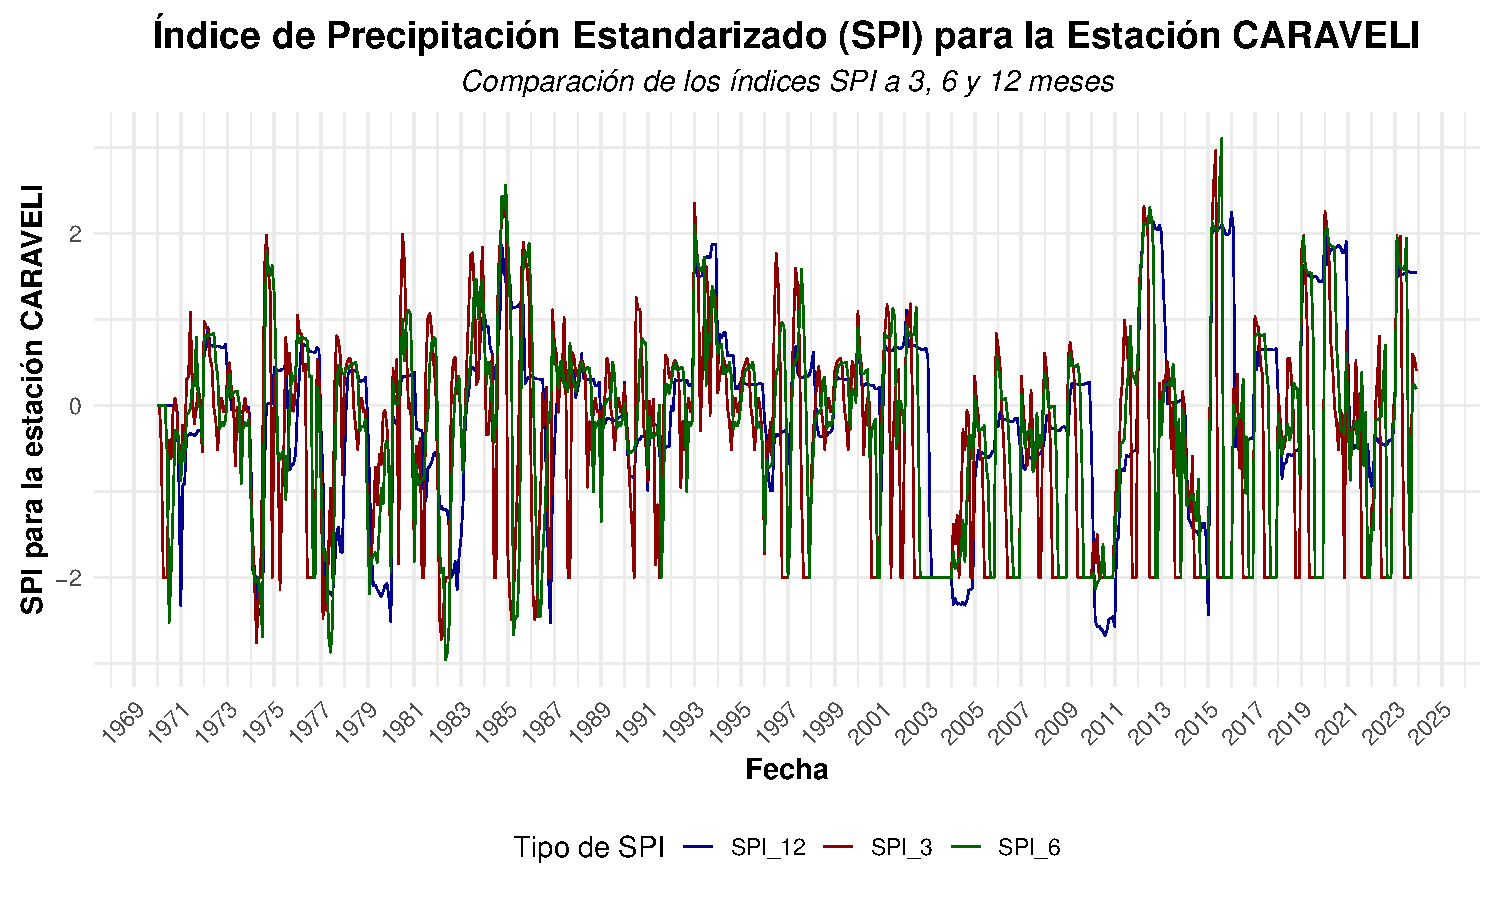
\includegraphics[width=\linewidth]{Capitulos/spi/SPI_Station_CARAVELI.pdf}
    
\end{minipage} \hfill
\begin{minipage}{0.45\textwidth}
    \centering
    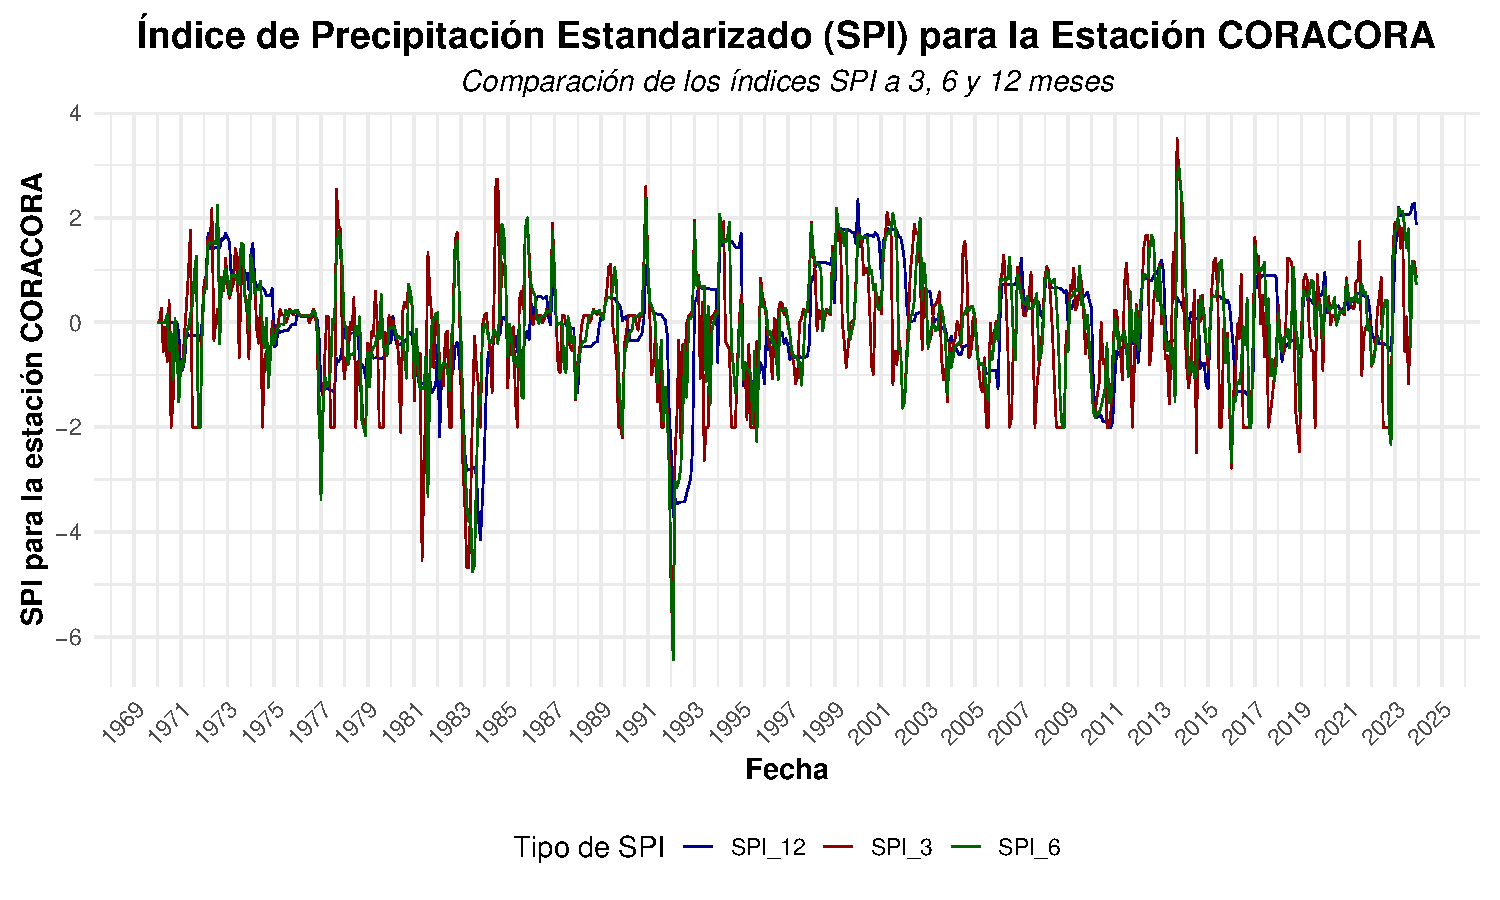
\includegraphics[width=\linewidth]{Capitulos/spi/SPI_Station_CORACORA.pdf}
   
\end{minipage}

\vskip\baselineskip  % Espacio entre filas de subgráficas

% Tercera fila de gráficas
\begin{minipage}{0.45\textwidth}
    \centering
    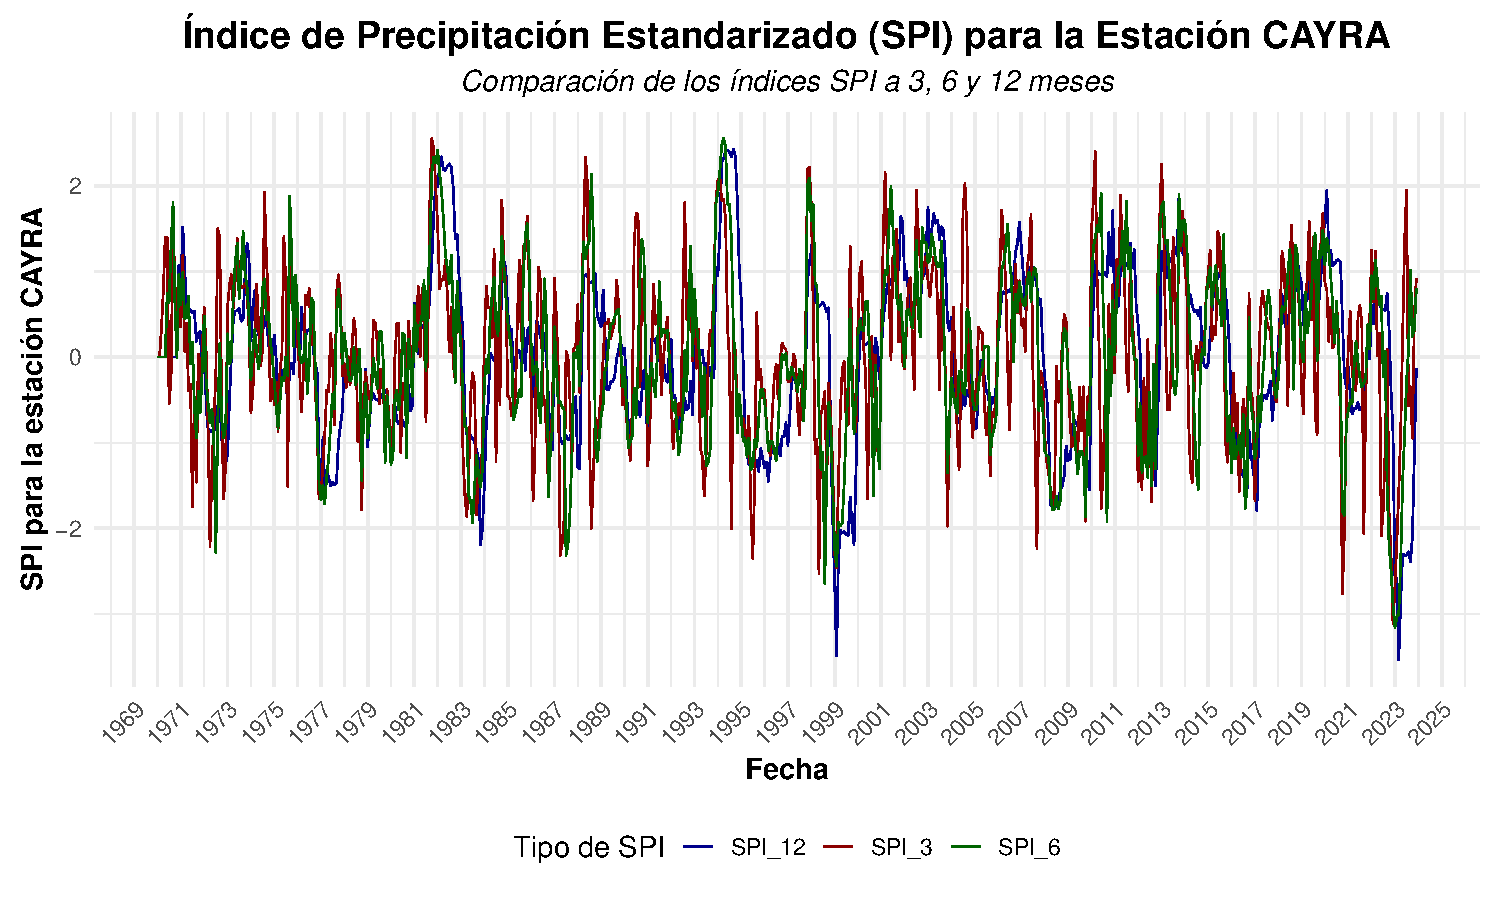
\includegraphics[width=\linewidth]{Capitulos/spi/SPI_Station_CAYRA.pdf}
    
\end{minipage} \hfill
\begin{minipage}{0.45\textwidth}
    \centering
    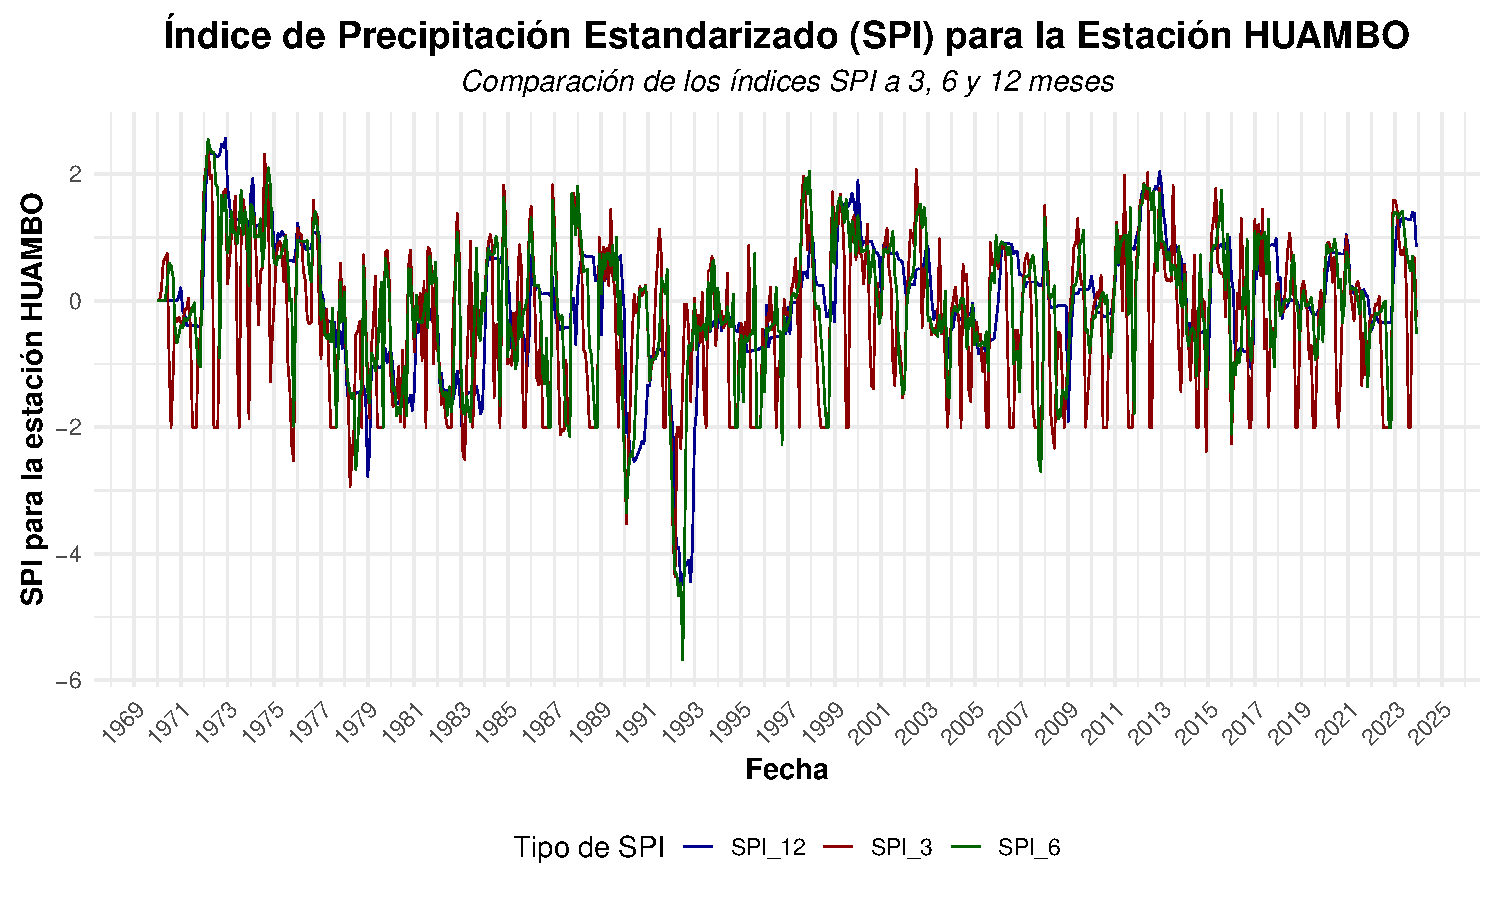
\includegraphics[width=\linewidth]{Capitulos/spi/SPI_Station_HUAMBO.pdf}
   
\end{minipage} \hfill
\begin{minipage}{0.45\textwidth}
    \centering
    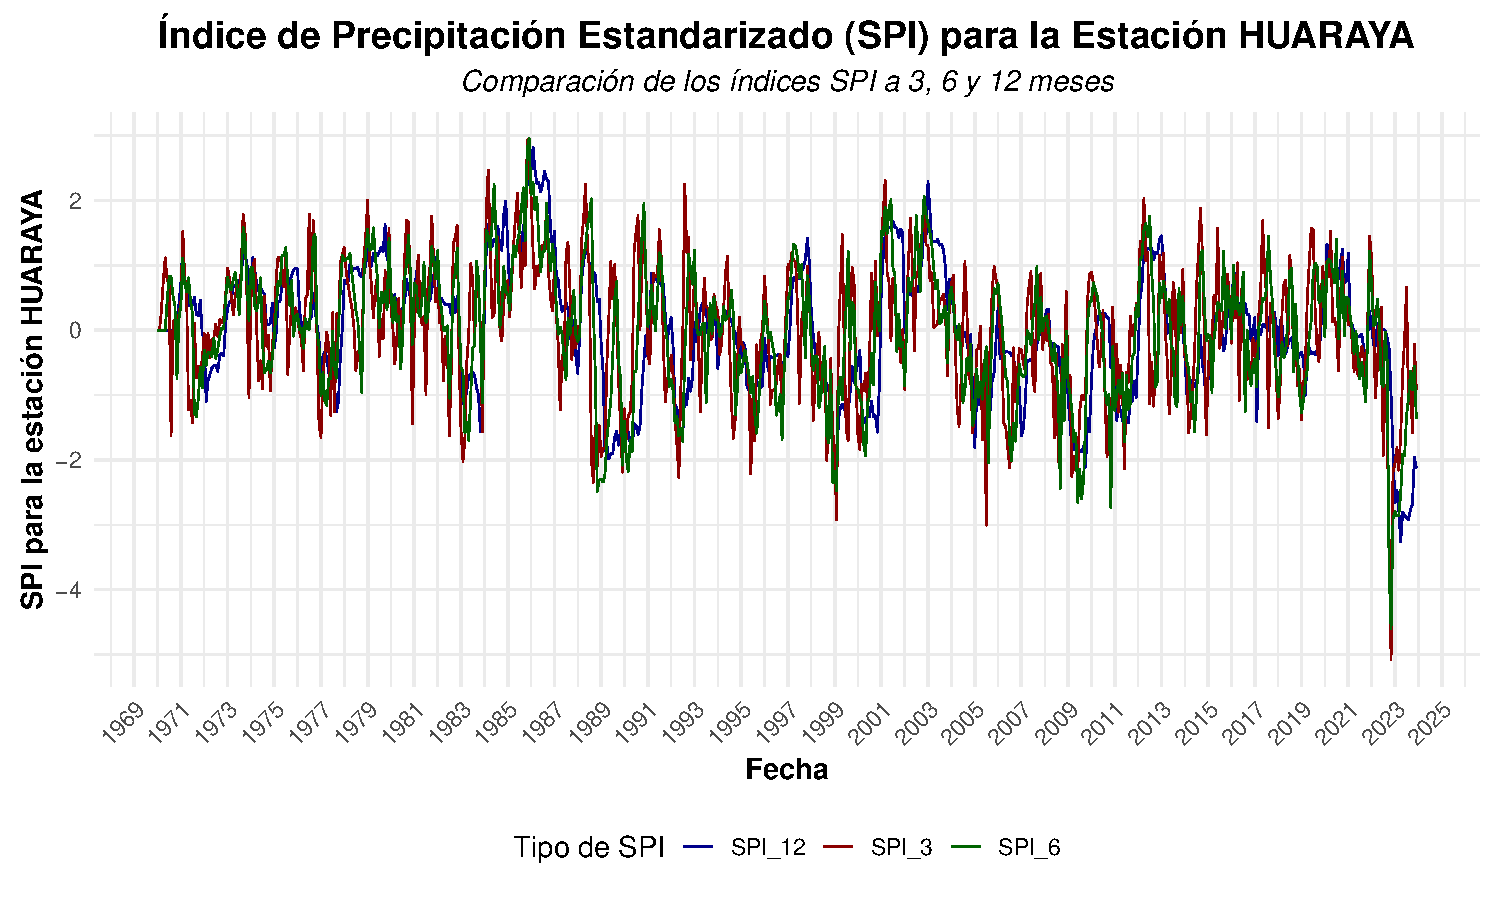
\includegraphics[width=\linewidth]{Capitulos/spi/SPI_Station_HUARAYA.pdf}
   
\end{minipage}

\vskip\baselineskip  % Espacio entre filas de subgráficas

% Cuarta fila de gráficas
\begin{minipage}{0.45\textwidth}
    \centering
    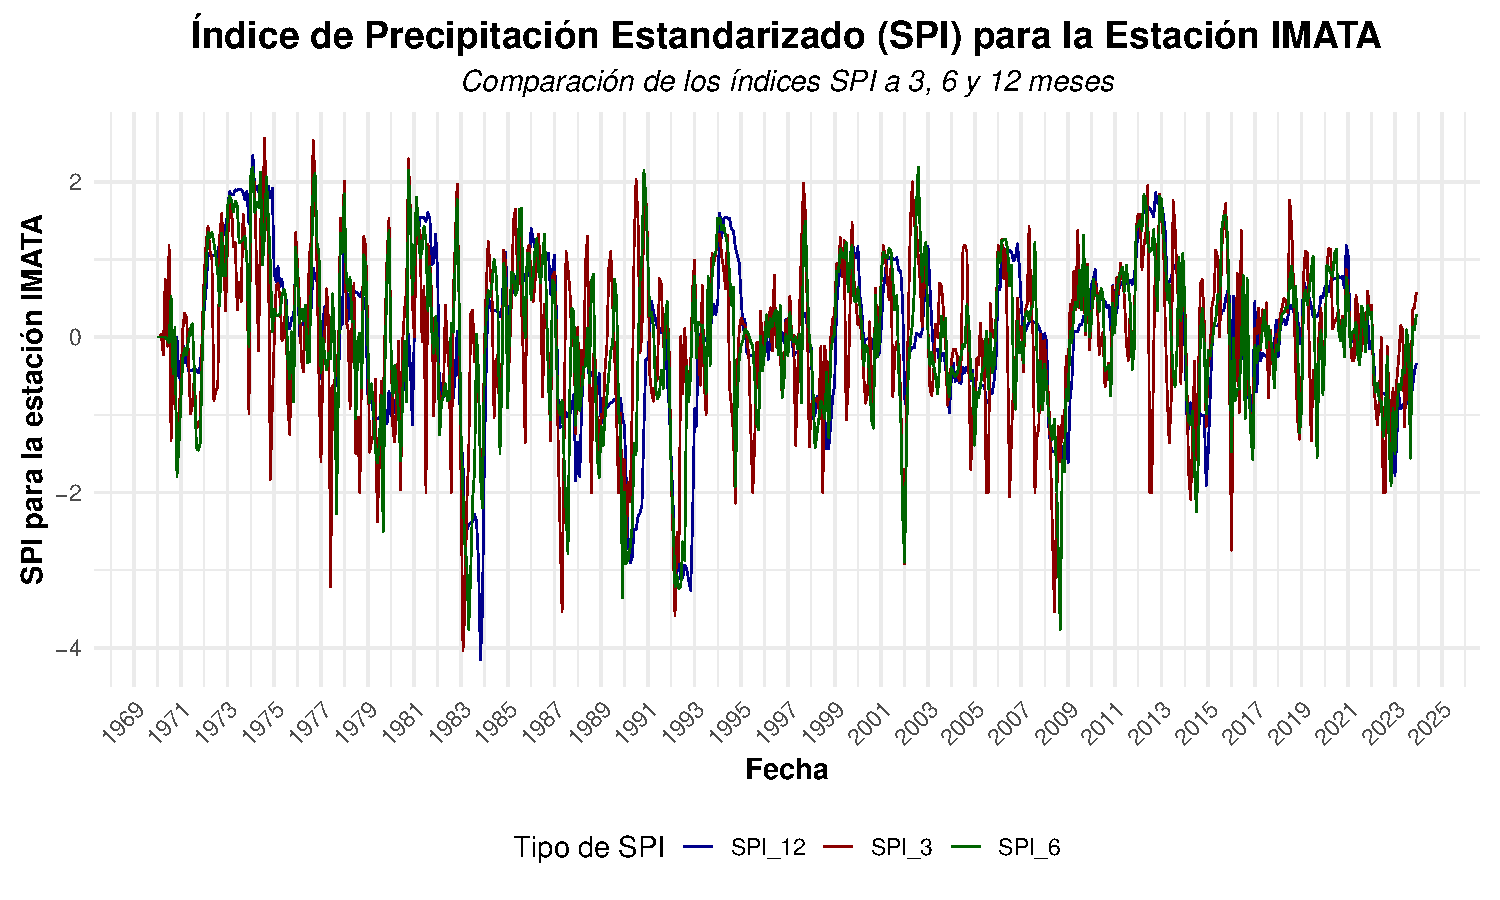
\includegraphics[width=\linewidth]{Capitulos/spi/SPI_Station_IMATA.pdf}
   
\end{minipage} \hfill
\begin{minipage}{0.45\textwidth}
    \centering
    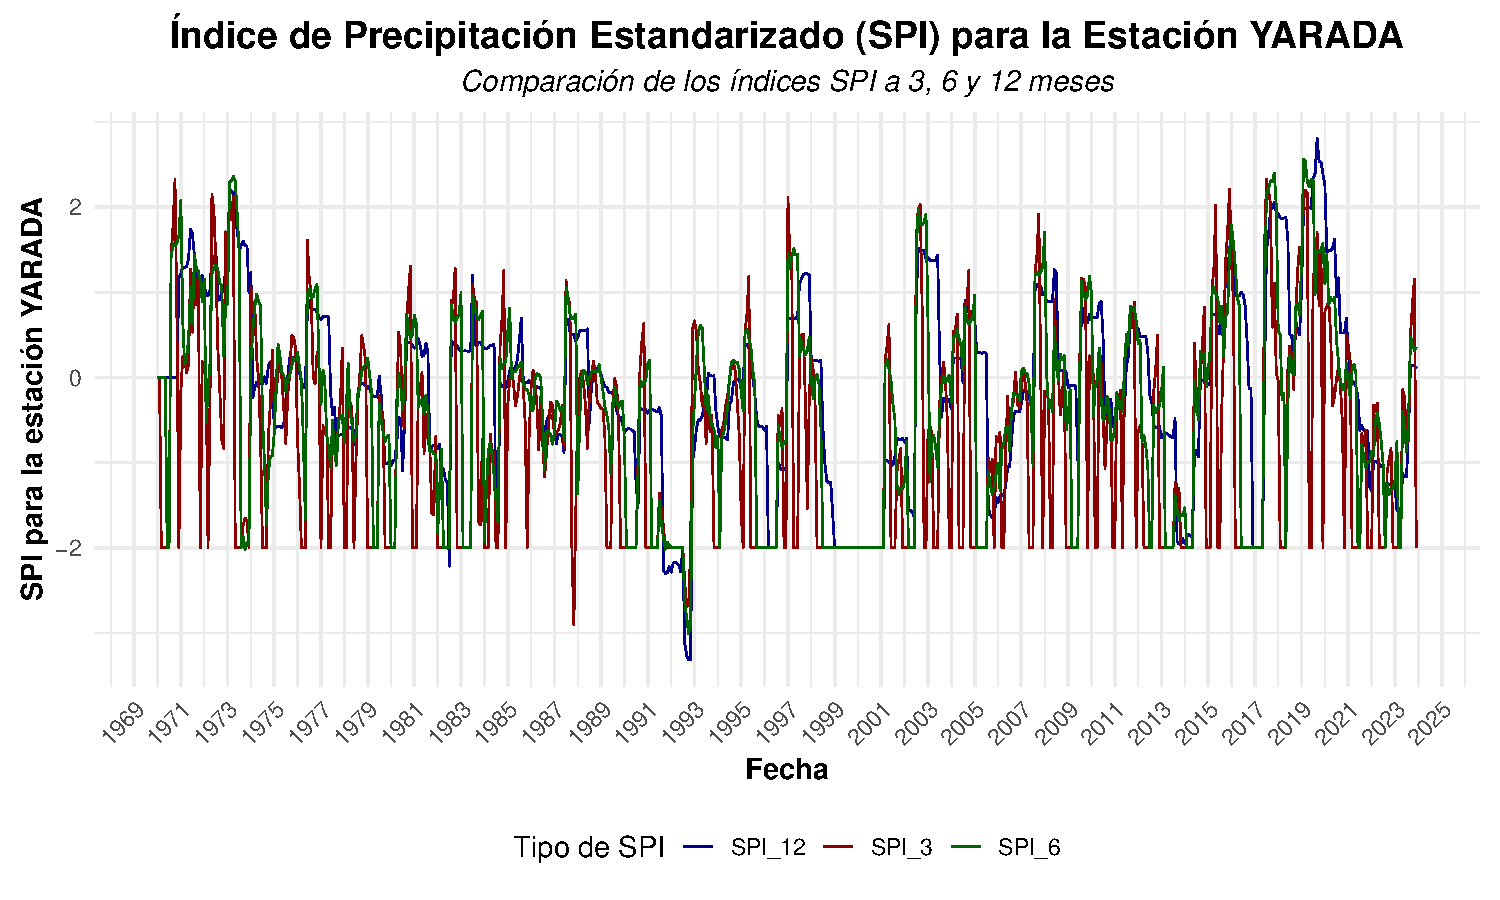
\includegraphics[width=\linewidth]{Capitulos/spi/SPI_Station_YARADA.pdf}
    
\end{minipage} \hfill
\begin{minipage}{0.45\textwidth}
    \centering
    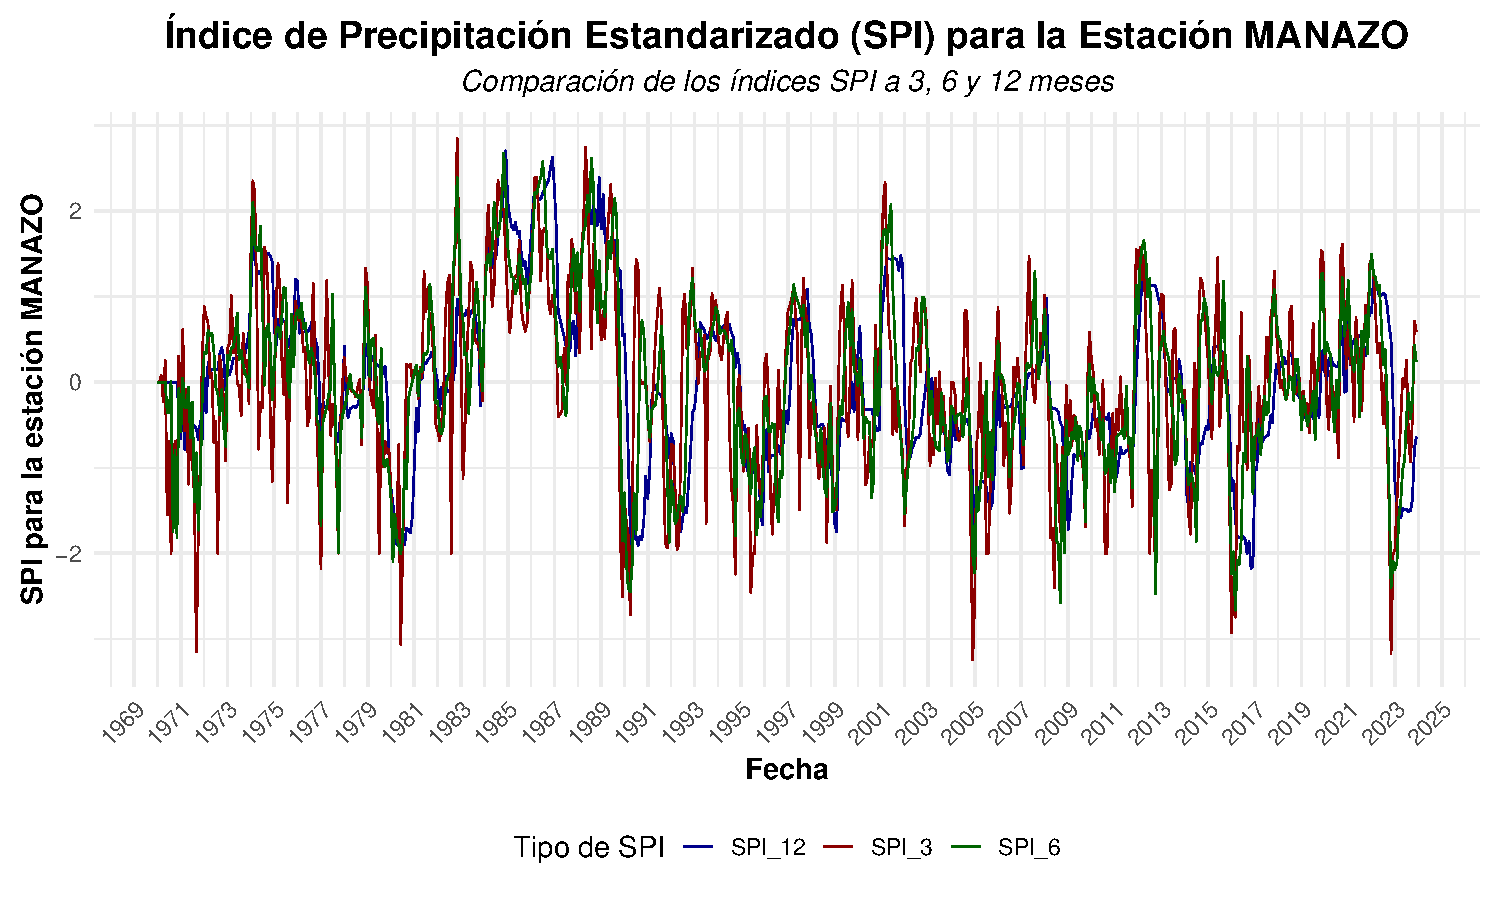
\includegraphics[width=\linewidth]{Capitulos/spi/SPI_Station_MANAZO.pdf}
   
\end{minipage}

\end{figure}
\end{landscape}

% Página 2
\begin{landscape}  % Continuar con orientación horizontal

\begin{figure}[h!]
\centering
% Quinta fila de gráficas
\begin{minipage}{0.45\textwidth}
    \centering
    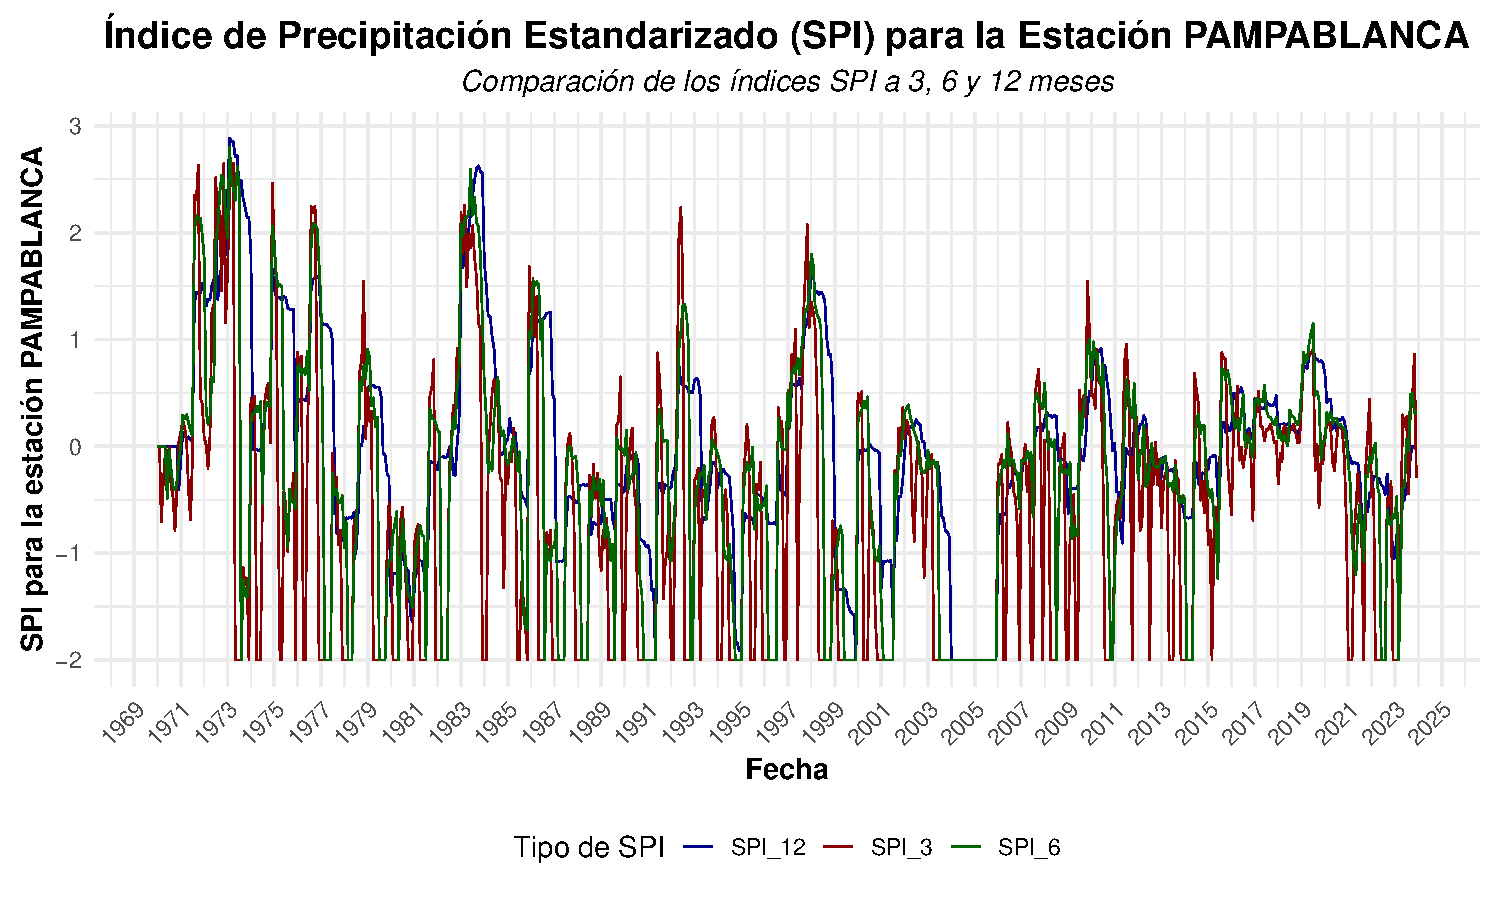
\includegraphics[width=\linewidth]{Capitulos/spi/SPI_Station_PAMPABLANCA.pdf}
  
\end{minipage} \hfill
\begin{minipage}{0.45\textwidth}
    \centering
    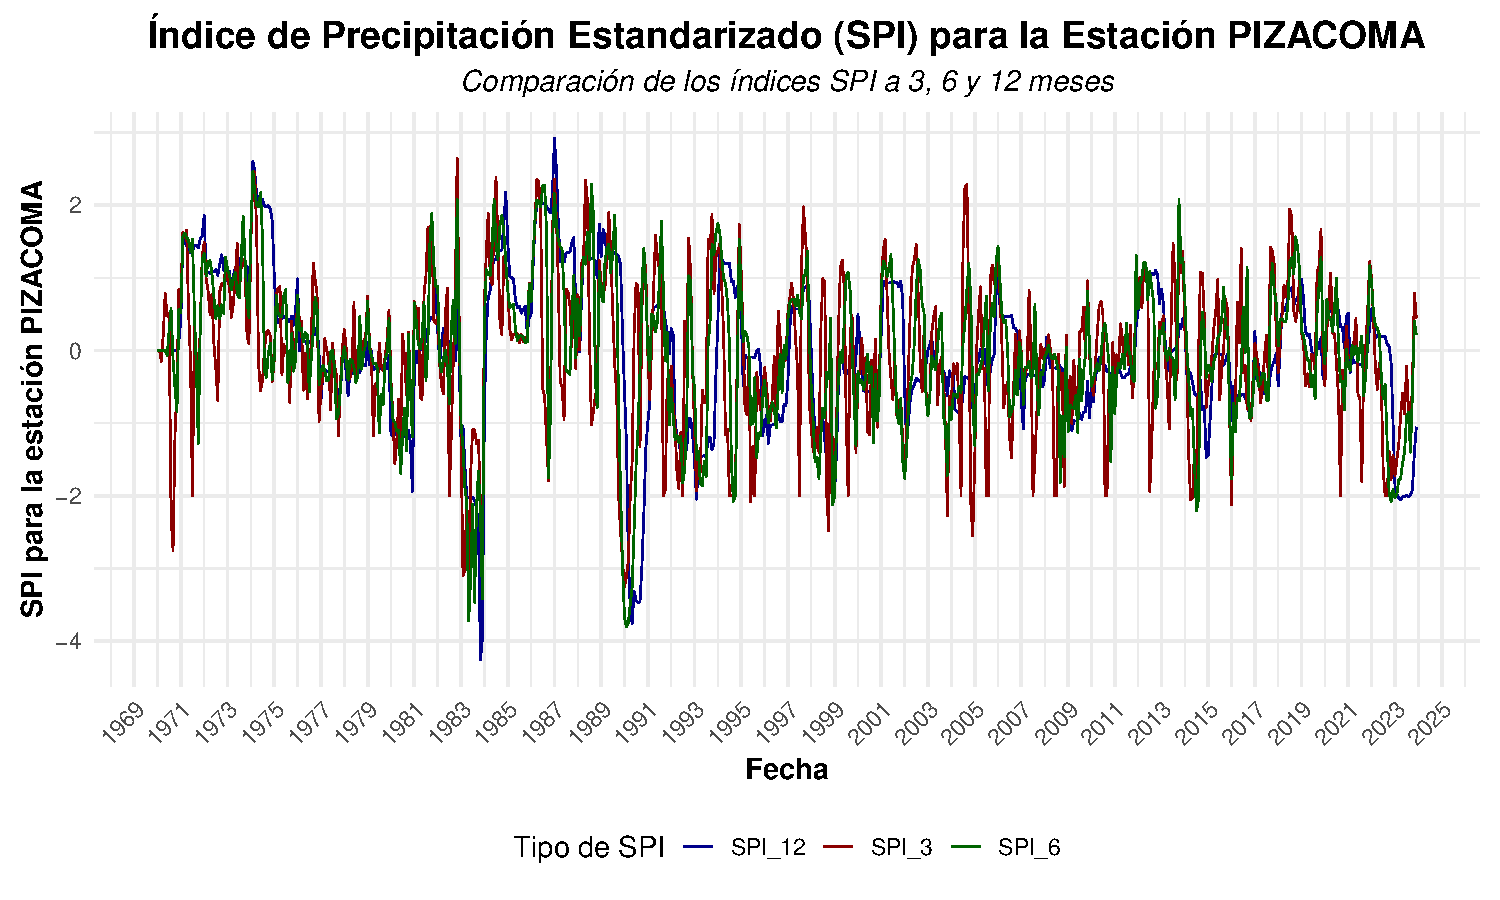
\includegraphics[width=\linewidth]{Capitulos/spi/SPI_Station_PIZACOMA.pdf}
    
\end{minipage} \hfill
\begin{minipage}{0.45\textwidth}
    \centering
    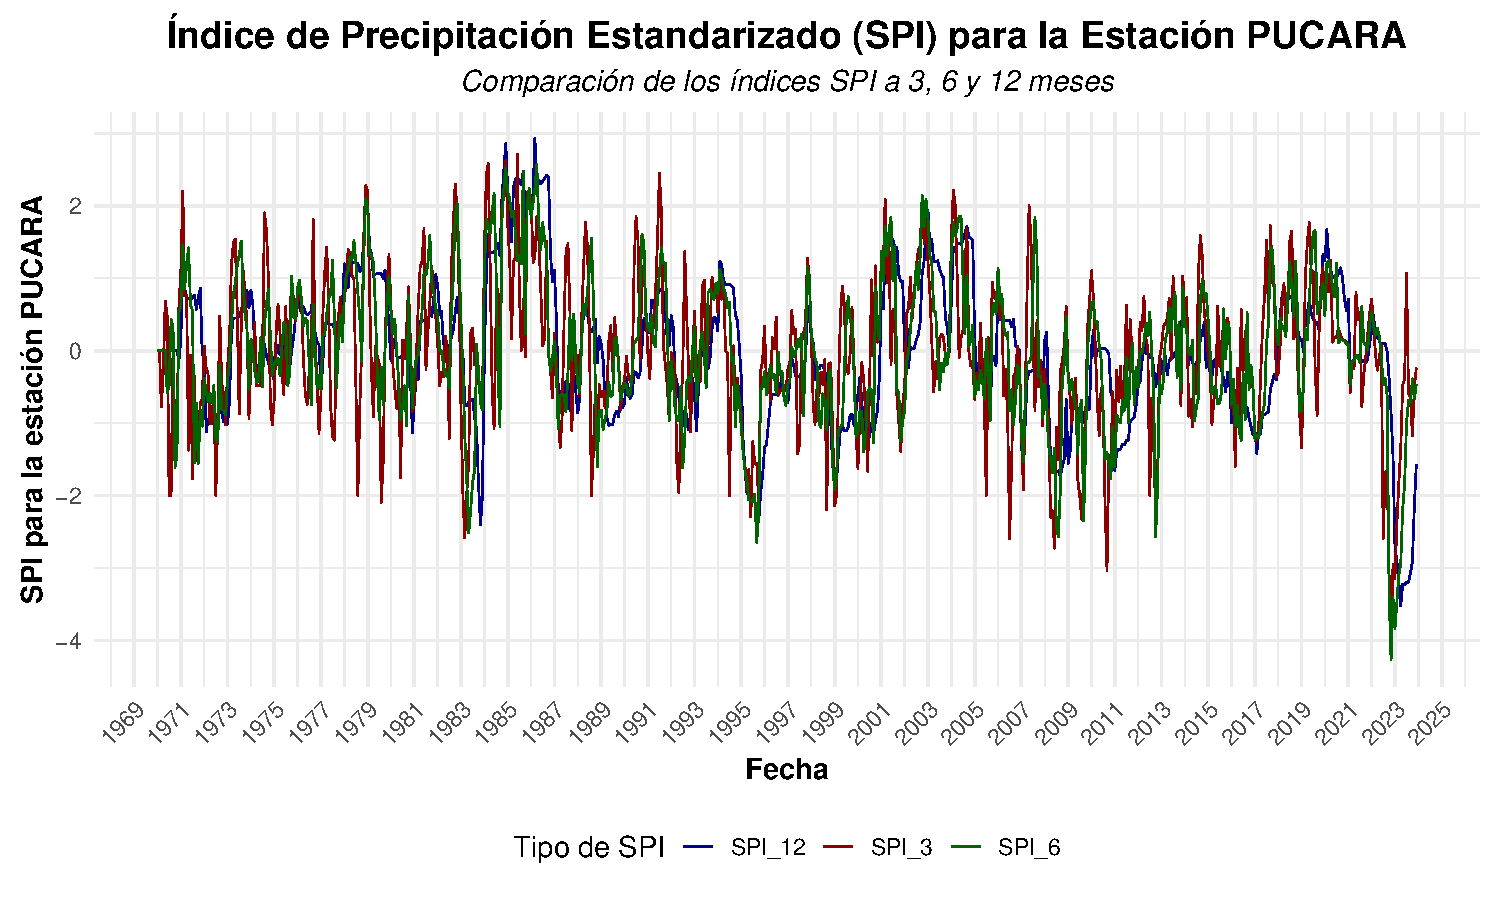
\includegraphics[width=\linewidth]{Capitulos/spi/SPI_Station_PUCARA.pdf}
   
\end{minipage}

\vskip\baselineskip  % Espacio entre filas de subgráficas

% Sexta fila de gráficas
\begin{minipage}{0.45\textwidth}
    \centering
    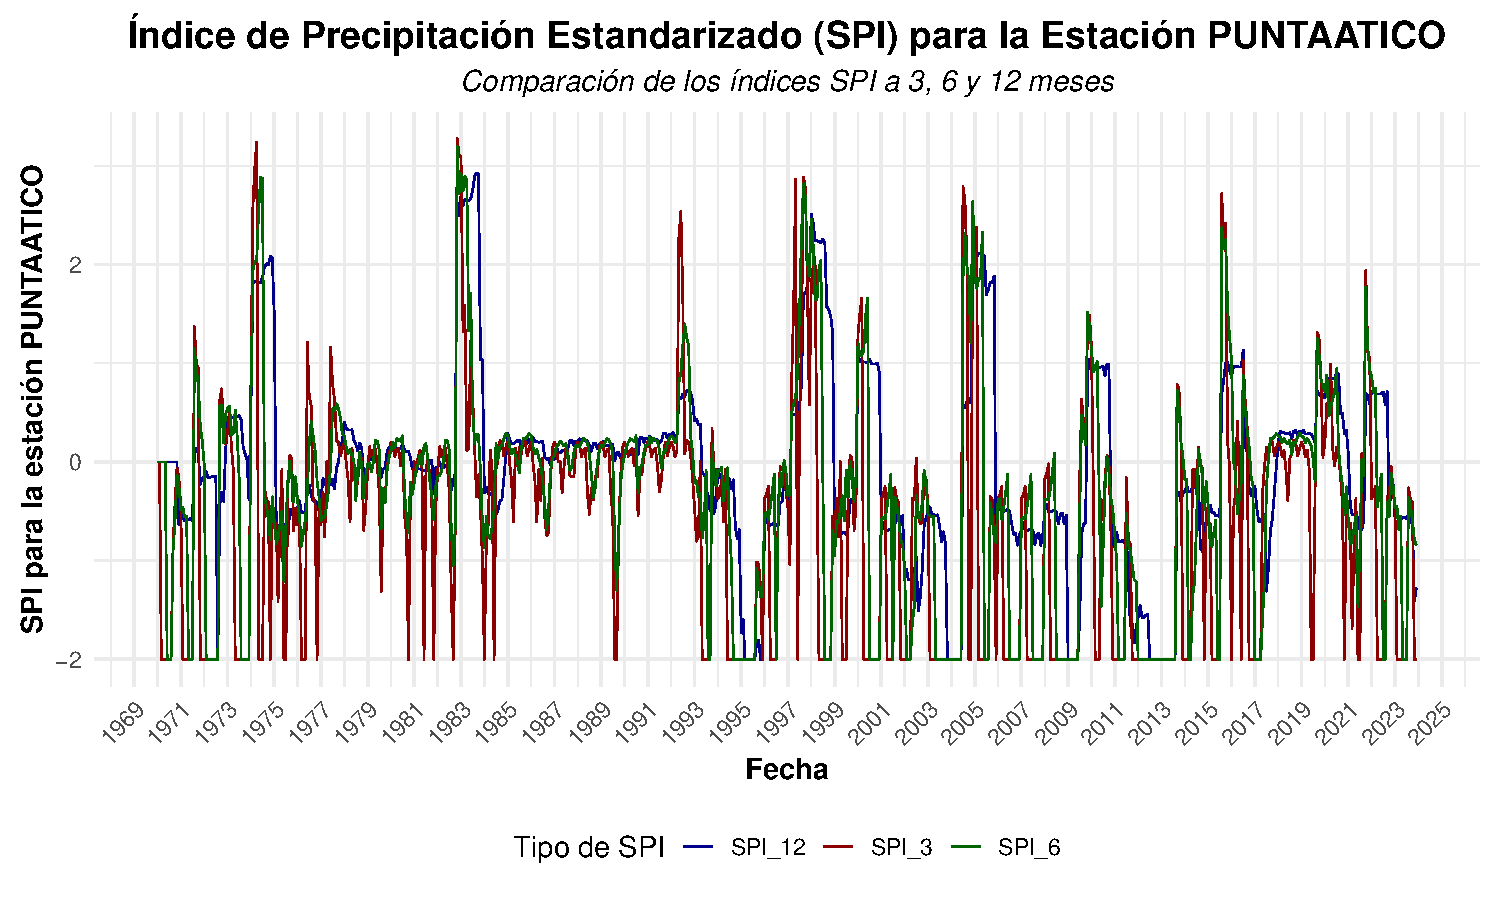
\includegraphics[width=\linewidth]{Capitulos/spi/SPI_Station_PUNTAATICO.pdf}
   
\end{minipage} \hfill
\begin{minipage}{0.45\textwidth}
    \centering
    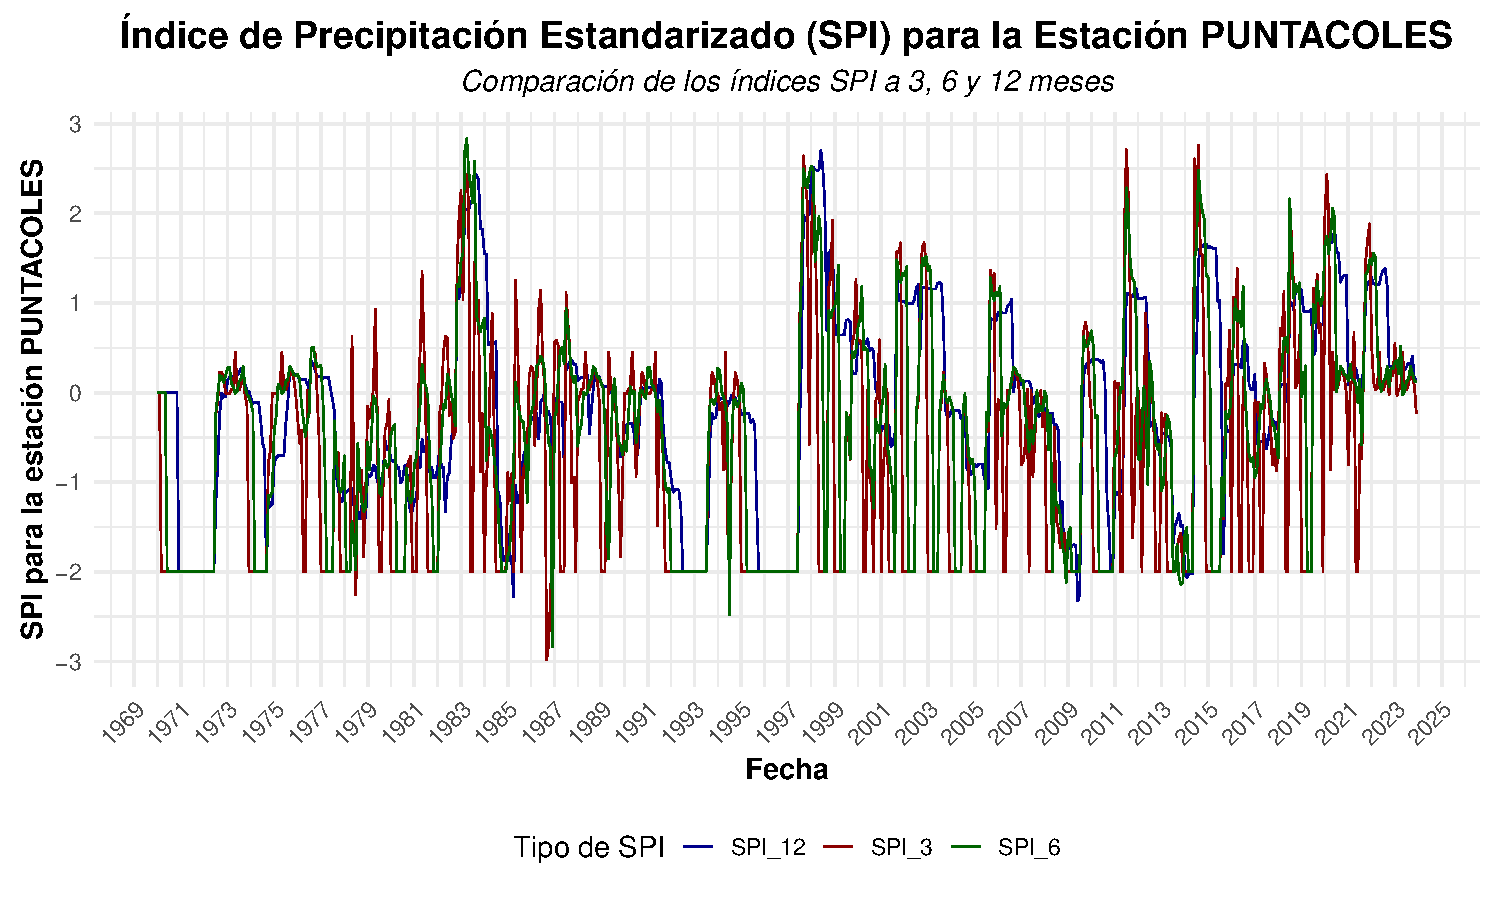
\includegraphics[width=\linewidth]{Capitulos/spi/SPI_Station_PUNTACOLES.pdf}
   
\end{minipage} \hfill
\begin{minipage}{0.45\textwidth}
    \centering
    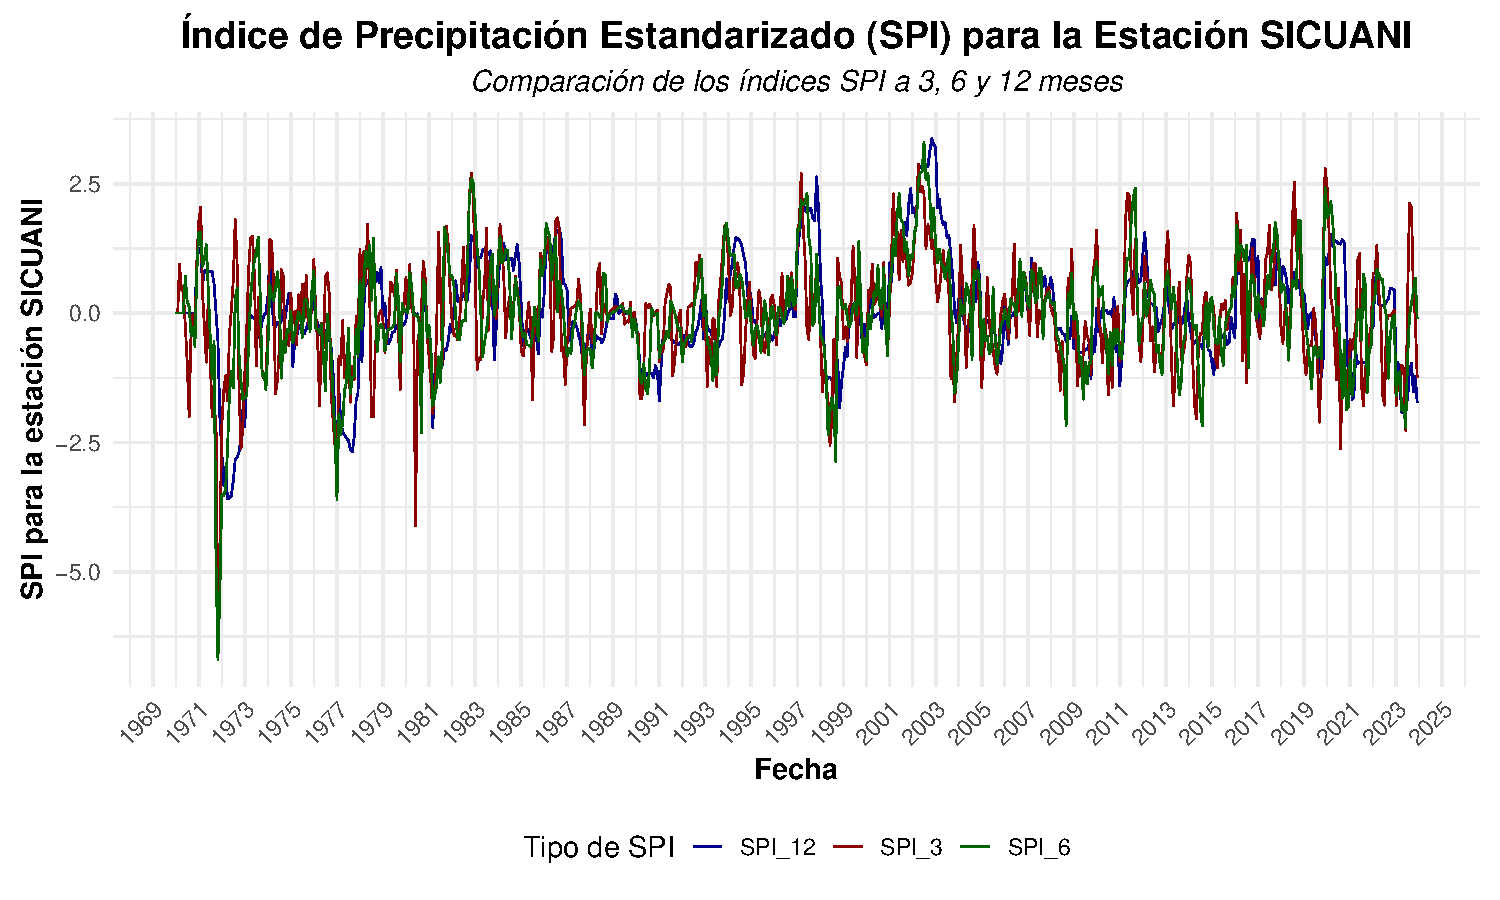
\includegraphics[width=\linewidth]{Capitulos/spi/SPI_Station_SICUANI.pdf}
   
\end{minipage}

\vskip\baselineskip  % Espacio entre filas de subgráficas

% Séptima fila de gráficas
\begin{minipage}{0.45\textwidth}
    \centering
    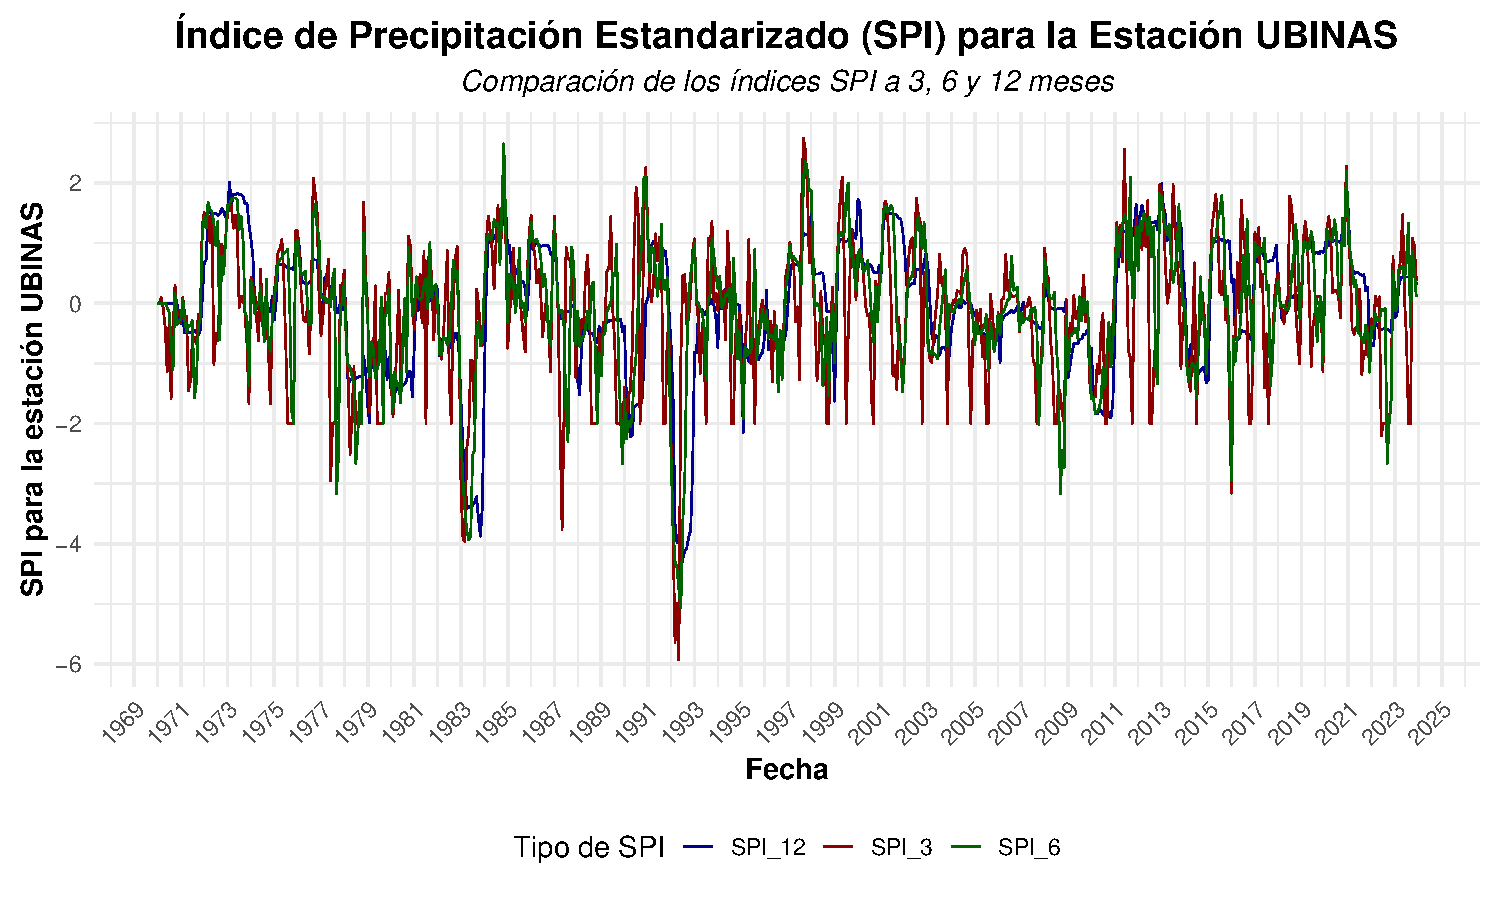
\includegraphics[width=\linewidth]{Capitulos/spi/SPI_Station_UBINAS.pdf}
 
\end{minipage}
\end{figure}

\end{landscape}

\subsection{Análisis de los Índices SPI para las Estaciones}


\subsection*{Estación \textit{ANCACHURO}}

La gráfica para la estación \textit{ANCACHURO} muestra la variabilidad de las precipitaciones a través de los tres índices SPI (3, 6 y 12 meses). El SPI a 3 meses refleja fluctuaciones con períodos de **sequía moderada** seguidos de fases más húmedas. El SPI a 6 y 12 meses indican una tendencia más estable, con algunos períodos de sequía moderada, pero mayormente en la categoría **normal**.

\subsection*{Estación \textit{ANDAHUAYLAS}}

El gráfico para la estación \textit{ANDAHUAYLAS} muestra fluctuaciones en las precipitaciones, con el SPI a 3 meses alcanzando **condiciones de sequía moderada** en varios períodos. El SPI a 6 y 12 meses son más estables, aunque también muestran momentos de **sequía severa** y condiciones más húmedas en algunos intervalos.

\subsection*{Estación \textit{CANDAVARE}}

Para la estación \textit{CANDAVARE}, el gráfico muestra fluctuaciones de SPI en los tres períodos. El SPI a 3 meses tiene varios picos hacia **sequía moderada**, con algunos intervalos de humedad. El SPI a 6 y 12 meses son más estables, aunque presentan caídas hacia la zona de sequía moderada en ciertos momentos.

\subsection*{Estación \textit{CARAVELI}}

La estación \textit{CARAVELI} muestra una tendencia similar en los tres SPI, con picos hacia **sequía** en el SPI a 3 meses. El SPI a 6 y 12 meses presentan una variabilidad más moderada, pero también reflejan períodos secos, especialmente en los primeros años del gráfico.

\subsection*{Estación \textit{CAYRA}}

En la estación \textit{CAYRA}, el SPI a 3 meses refleja fluctuaciones significativas, con momentos de **sequía moderada** y **condiciones húmedas** intercaladas. El SPI a 6 meses tiene una tendencia más estable, mientras que el SPI a 12 meses muestra un comportamiento equilibrado, con períodos secos moderados seguidos de condiciones normales.

\subsection*{Estación \textit{CORACORA}}

El gráfico de la estación \textit{CORACORA} muestra fluctuaciones en los tres índices SPI. El SPI a 3 meses refleja varios períodos de **sequía severa**. El SPI a 6 y 12 meses también presentan caídas hacia la zona de sequía, pero la tendencia general es más estable, con algunos intervalos de humedad en el largo plazo.

\subsection*{Estación \textit{COTAHUASI}}

En la estación \textit{COTAHUASI}, el gráfico muestra un comportamiento variable en los tres períodos de SPI. El SPI a 3 meses presenta varios períodos de **sequía severa**, mientras que el SPI a 6 meses es más estable, pero también muestra fluctuaciones negativas. El SPI a 12 meses muestra una tendencia moderada, con algunos picos de sequía prolongada.

\subsection*{Estación \textit{HUAMBO}}

El gráfico de la estación \textit{HUAMBO} refleja fluctuaciones en los tres SPI, con algunos picos de **sequía severa** en el SPI a 3 meses. El SPI a 6 y 12 meses son más estables, pero presentan caídas hacia la categoría de sequía moderada, con algunos intervalos secos prolongados en la estación.

\subsection*{Estación \textit{HUARAYA}}

La estación \textit{HUARAYA} muestra fluctuaciones tanto en el SPI a 3 meses como en el SPI a 6 y 12 meses. El SPI a 3 meses refleja fluctuaciones hacia valores negativos, lo que indica **sequía moderada**. El SPI a 6 y 12 meses son más estables, aunque también muestran momentos secos, pero con una tendencia general más equilibrada.


\subsection*{Estación \textit{IMATA}}

La gráfica para la estación \textit{IMATA} muestra un comportamiento de las precipitaciones con fluctuaciones evidentes en los tres períodos de SPI. El SPI a 3 meses muestra picos negativos en los primeros años, lo que sugiere condiciones de **sequía severa**. El SPI a 6 y 12 meses refleja una tendencia más estable, pero también presenta valores negativos en algunas ocasiones, indicando sequía moderada y **condiciones húmedas** en ciertos períodos.

\subsection*{Estación \textit{MANAZO}}

El gráfico para la estación \textit{MANAZO} muestra un comportamiento variable en los tres índices SPI. El SPI a 3 meses tiene fluctuaciones hacia los valores negativos, lo que indica **sequía**. El SPI a 6 meses es más estable, pero también presenta caídas a valores negativos. El SPI a 12 meses muestra una tendencia equilibrada, con algunos períodos de **sequía severa** y otros más húmedos.

\subsection*{Estación \textit{PAMPABLANCA}}

La estación \textit{PAMPABLANCA} muestra en su gráfico un comportamiento más seco, con picos negativos en los tres períodos de SPI. El SPI a 3 meses refleja **sequía severa**, especialmente en los primeros años. El SPI a 6 y 12 meses también presentan valores negativos, lo que sugiere que la estación experimentó **sequías prolongadas** en la mayor parte del tiempo.

\subsection*{Estación \textit{PIZACOMA}}

En la estación \textit{PIZACOMA}, el SPI de 3 meses refleja fluctuaciones significativas, con algunos picos en valores negativos. El SPI a 6 y 12 meses son más estables, pero también muestran intervalos de **sequía moderada**. En general, la estación experimentó períodos secos intercalados con condiciones más normales.

\subsection*{Estación \textit{PUCARA}}

La gráfica para la estación \textit{PUCARA} muestra un comportamiento más estable en el SPI a 6 y 12 meses, mientras que el SPI a 3 meses muestra algunas fluctuaciones significativas. El SPI a 6 y 12 meses indican **condiciones normales** en la mayoría del tiempo, con solo algunos episodios más secos, aunque con una tendencia positiva en los últimos años.

\subsection*{Estación \textit{PUNTAATICO}}

El gráfico para la estación \textit{PUNTAATICO} refleja fluctuaciones en las precipitaciones con los tres índices SPI. El SPI a 3 meses muestra un comportamiento variable, con varios períodos de **sequía moderada**. El SPI a 6 meses es más estable, pero con algunas caídas hacia valores negativos. El SPI a 12 meses muestra una tendencia más equilibrada, con algunos picos hacia **condiciones húmedas**.

\subsection*{Estación \textit{PUNTACOLES}}

Para la estación \textit{PUNTACOLES}, el gráfico muestra fluctuaciones en los tres períodos de SPI. El SPI a 3 meses presenta **sequía severa** en varios períodos, mientras que el SPI a 6 y 12 meses muestran una tendencia más equilibrada. La estación experimenta algunos momentos de sequía, pero también fases más húmedas.

\subsection*{Estación \textit{SICUANI}}

En la estación \textit{SICUANI}, el gráfico muestra fluctuaciones en el SPI a 3 meses, con algunos períodos de **sequía** y condiciones normales. El SPI a 6 meses es más estable, con algunos picos hacia valores negativos. El SPI a 12 meses muestra una tendencia más equilibrada, con intervalos secos intercalados con condiciones húmedas.

\subsection*{Estación \textit{UBINAS}}

Para la estación \textit{UBINAS}, el gráfico muestra una tendencia variable en los tres índices SPI. El SPI a 3 meses muestra algunos picos de **sequía severa**, especialmente hacia el final del período. El SPI a 6 y 12 meses presentan una tendencia más estable, con intervalos de **sequía moderada** seguidos de valores cercanos a lo normal.

\subsection*{Estación \textit{YARADA}}

El gráfico para la estación \textit{YARADA} muestra fluctuaciones en el SPI a 3 meses, con algunos picos de sequía, seguidos de algunos intervalos más húmedos. El SPI a 6 y 12 meses tiene una tendencia más estable, pero también presenta caídas hacia valores negativos, lo que indica episodios de **sequía moderada** y otras condiciones más húmedas.

\section{Análisis de Cópulas Bivariadas}

El análisis de cópulas bivariadas tiene como objetivo modelar la dependencia y la correlación entre las variables consideradas, en este caso, entre los índices de precipitación estandarizados (SPI) y otras variables climáticas, como la humedad relativa, la precipitación y la velocidad media del viento. Antes de realizar la construcción de cópulas bivariadas, es necesario llevar a cabo una serie de pasos preliminares que aseguren la adecuada integración y análisis de los datos.

En primer lugar, se debe realizar una **transformación de los datos** para que todas las variables involucradas estén en un formato adecuado para el análisis de cópulas. Esto implica la **normalización** de los datos para que las distribuciones de las variables sean independientes de las unidades de medida y, en muchos casos, sea necesario aplicar alguna **transformación marginal** para que las variables sigan distribuciones conocidas, como la distribución uniforme o normal.

Una vez que los datos han sido preprocesados y transformados adecuadamente, el siguiente paso es analizar la **dependencia bivariada** entre los índices SPI y las variables climáticas, como la **humedad relativa**, la **precipitación** y la **velocidad media del viento**. En este paso, se explora la **relación entre dos variables** a través del uso de cópulas bivariadas, que son herramientas estadísticas muy útiles para modelar la dependencia no lineal y explorar el tipo de relación entre las variables.

Las cópulas bivariadas permiten estudiar la dependencia entre dos variables sin asumir ninguna forma de relación lineal, lo que las convierte en una herramienta fundamental cuando se trata de variables que no siguen distribuciones estándar o en las cuales se sospecha que existen dependencias complejas. Las cópulas permiten separar el análisis de la **dependencia estructural** de las **distribuciones marginales** de las variables, lo que ofrece una gran flexibilidad en el modelado de datos multivariantes.

El análisis de las cópulas bivariadas se lleva a cabo mediante la elección de una **cópula adecuada** que describa correctamente la relación entre las variables SPI y las variables climáticas. Existen diversas cópulas, como la cópula de **Gaussian**, **Clayton**, **Gumbel**, entre otras, y la elección de la misma dependerá de la naturaleza de la dependencia observada en los datos. Además, se deben estimar los parámetros de la cópula seleccionada para asegurar que el modelo ajustado refleje correctamente la estructura de dependencia observada.

Una vez que se ha ajustado la cópula bivariada, se realiza una evaluación de su ajuste mediante **pruebas de bondad de ajuste**, como el **criterio de Akaike (AIC)** o el **criterio de Bayes (BIC)**, que permiten comparar distintos modelos y determinar cuál es el que mejor describe la dependencia entre las variables.

Finalmente, el análisis de cópulas bivariadas proporciona una visión más profunda de cómo las variables climáticas se interrelacionan con los índices SPI, lo cual es esencial para realizar **predicciones climáticas más precisas** y para comprender las **dinámicas de las precipitaciones y sus factores asociados**, lo que puede ser fundamental para estudios relacionados con la **gestión del agua**, **agricultura** o **cambio climático**.

\subsection{Estadisticos descriptivos de las variable en estudio}


\begin{table}[H]
\centering
\caption{Estadísticas de la Estación \textit{ANDAHUAYLAS}}  % Título de la tabla
\resizebox{1\textwidth}{!}{ % Ajuste de la tabla al tamaño deseado
\begin{tabular}{lccccccc}
\hline
\rowcolor{gray!20} \textbf{Statistics} & \textbf{PT} & \textbf{HR} & \textbf{TM} & \textbf{VTMED} & \textbf{SPI3} & \textbf{SPI6} & \textbf{SPI12} \\
\hline
\textit{n} & 648.0 & 648.0 & 648.0 & 648.0 & 648.0 & 648.0 & 648.0 \\
\textit{Minimum} & 0.0 & 57.4387 & 10.5461 & 0.62277 & -3.09023 & -2.80409 & -3.09023 \\
\textit{1st. Quartile} & 14.225 & 76.0823 & 12.4071 & 2.0998 & -0.898723 & -0.873861 & -0.423355 \\
\textit{Median} & 39.55 & 80.4458 & 13.6084 & 2.49623 & -0.0401171 & 0.065782 & 0.0321254 \\
\textit{Mean} & 54.5675 & 80.1822 & 13.4164 & 2.49402 & -0.0472496 & -0.0209047 & 0.00885161 \\
\textit{3rd. Quartile} & 88.0228 & 84.9611 & 14.3857 & 2.79065 & 0.905807 & 0.888012 & 0.618584 \\
\textit{Maximum} & 251.5 & 98.1972 & 16.5071 & 5.48198 & 2.38335 & 2.19683 & 2.83169 \\
\textit{Rank} & 251.5 & 40.7585 & 5.96098 & 4.85921 & 5.47358 & 5.00093 & 5.92192 \\
\textit{Interquartile Rank} & 73.7978 & 8.87882 & 1.97857 & 0.69085 & 1.80453 & 1.76187 & 1.04194 \\
\textit{Variance} & 2450.01 & 44.8424 & 1.61868 & 0.421805 & 1.2303 & 1.13404 & 1.01948 \\
\textit{Standard Deviation} & 49.4975 & 6.69645 & 1.27227 & 0.649465 & 1.10919 & 1.06491 & 1.0097 \\
\textit{Variation Coeff.} & 0.907089 & 0.0835155 & 0.09483 & 0.260409 & -23.4751 & -50.9414 & 114.069 \\
\textit{Skewness} & 1.06463 & -0.236198 & -0.256999 & 0.683784 & -0.213414 & -0.220901 & -0.834186 \\
\textit{Kurtosis} & 0.63867 & -0.191435 & -0.805296 & 2.60374 & -0.654145 & -0.919708 & 1.63032 \\
\hline
\end{tabular}
\label{tab:stat_desc_and}
}
\end{table}


Los resultados obtenidos a partir de las estadísticas descriptivas (Tabla \ref{tab:stat_desc_and}) y las matrices de correlación (Figura \ref{fig:corr_and}) para la estación \textit{Andahuaylas} ofrecen una visión detallada sobre las relaciones entre las variables meteorológicas y los índices de precipitación estandarizada. Se destaca que ciertas variables presentan una dependencia lineal significativa, como la correlación entre la humedad relativa (HR) y el índice de precipitación estandarizada a 3 meses (SPI3), lo que indica que estas variables están fuertemente relacionadas y, por tanto, podrían ser modeladas eficazmente utilizando cópulas elípticas, como la cópula normal. En contraste, otras combinaciones de variables, como SPI6 y SPI12, muestran dependencias no lineales, por lo que una cópula arquimediana, como la cópula de Clayton o Gumbel, sería más adecuada para capturar la naturaleza asimétrica de estas relaciones. Adicionalmente, la velocidad media del viento (VTMED) tiene una relación débil con las demás variables, lo que sugiere que en este caso se podría considerar el uso de cópulas independientes o cópulas con parámetros bajos de dependencia. %En conclusión, los resultados de este análisis proporcionan una base sólida para la selección de cópulas apropiadas, permitiendo modelar las dependencias bivariadas de las variables en función de sus características de dependencia lineales o no lineales.









\begin{figure}[H]
\centering
\caption{Gráficas de dispersión para la Estación \textit{ANDAHUAYLAS}}
\begin{minipage}{0.33\textwidth}
    \centering
    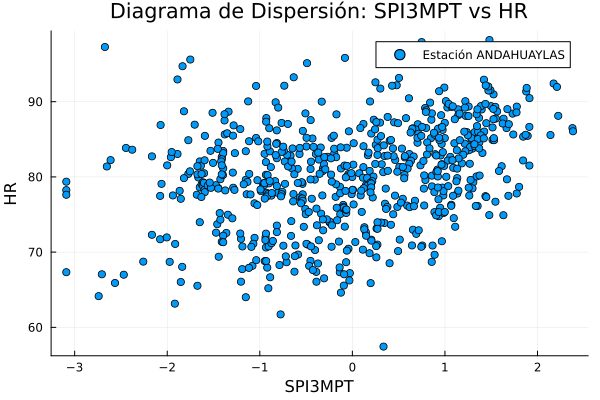
\includegraphics[width=\linewidth]{Capitulos/Scaterplot/ANDAHUAYLAS_SPI3MPT_vs_HR.png}
    \subcaption{SPI3MPT vs HR}
\end{minipage}\hfill
\begin{minipage}{0.33\textwidth}
    \centering
    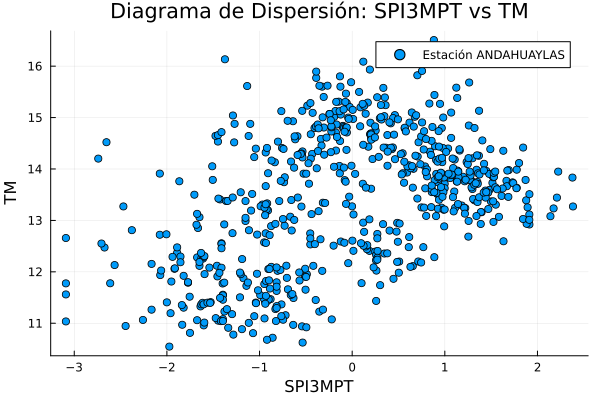
\includegraphics[width=\linewidth]{Capitulos/Scaterplot/ANDAHUAYLAS_SPI3MPT_vs_TM.png}
    \subcaption{SPI3MPT vs TM}
\end{minipage}\hfill
\begin{minipage}{0.33\textwidth}
    \centering
    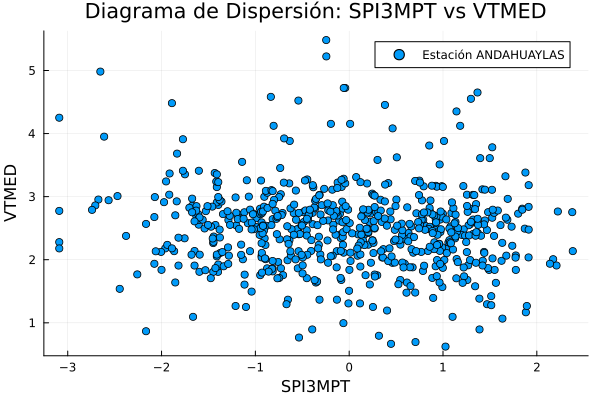
\includegraphics[width=\linewidth]{Capitulos/Scaterplot/ANDAHUAYLAS_SPI3MPT_vs_VTMED.png}
    \subcaption{SPI3MPT vs VTMED}
\end{minipage}

\vspace{0.3cm}  % Espacio entre filas de subgráficas

\begin{minipage}{0.33\textwidth}
    \centering
    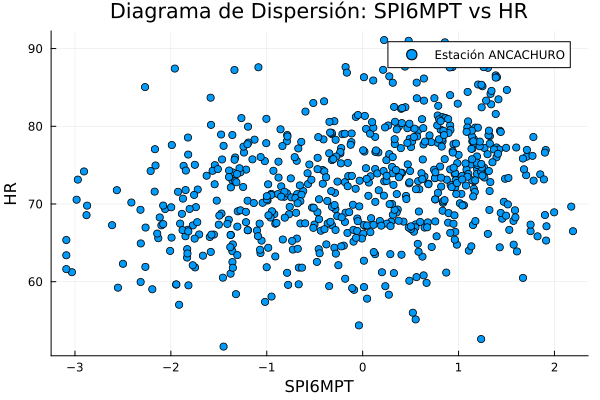
\includegraphics[width=\linewidth]{Capitulos/Scaterplot/ANCACHURO_SPI6MPT_vs_HR.png}
    \subcaption{SPI6MPT vs HR}
\end{minipage}\hfill
\begin{minipage}{0.33\textwidth}
    \centering
    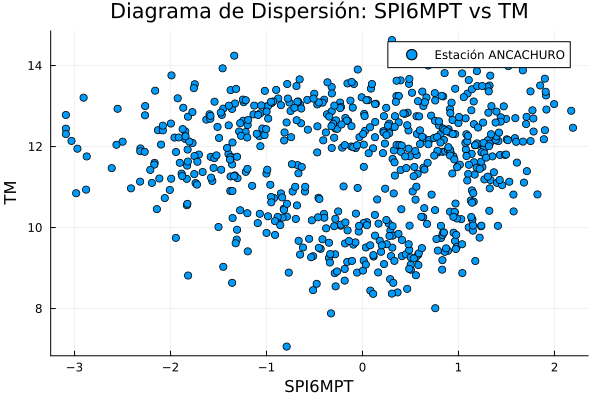
\includegraphics[width=\linewidth]{Capitulos/Scaterplot/ANCACHURO_SPI6MPT_vs_TM.png}
    \subcaption{SPI6MPT vs TM}
\end{minipage}\hfill
\begin{minipage}{0.33\textwidth}
    \centering
    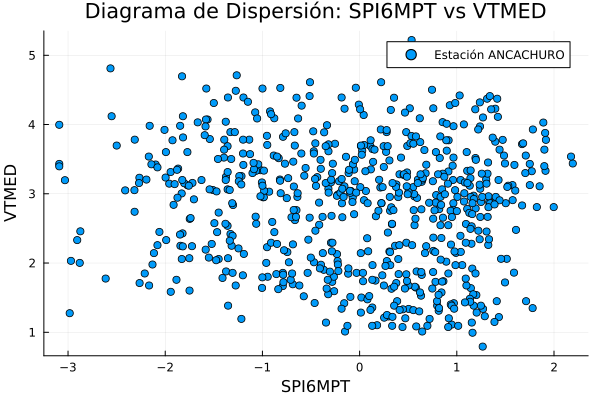
\includegraphics[width=\linewidth]{Capitulos/Scaterplot/ANCACHURO_SPI6MPT_vs_VTMED.png}
    \subcaption{SPI6MPT vs VTMED}
\end{minipage}

\vspace{0.3cm}  % Espacio entre filas de subgráficas

\begin{minipage}{0.33\textwidth}
    \centering
    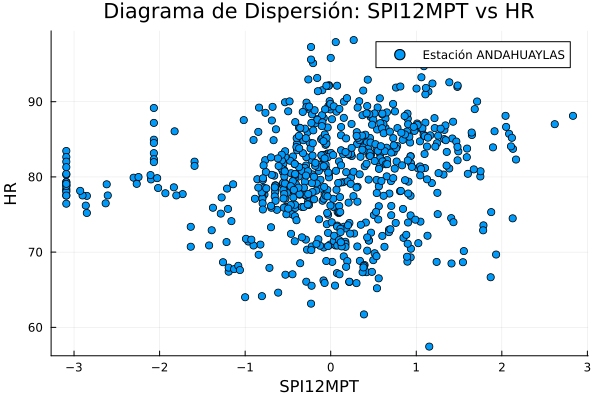
\includegraphics[width=\linewidth]{Capitulos/Scaterplot/ANDAHUAYLAS_SPI12MPT_vs_HR.png}
    \subcaption{SPI12MPT vs HR}
\end{minipage}\hfill
\begin{minipage}{0.33\textwidth}
    \centering
    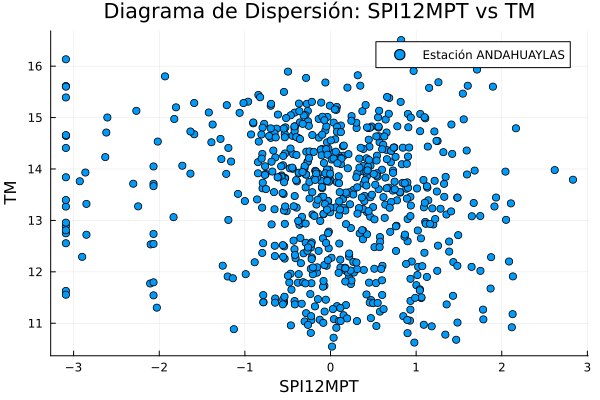
\includegraphics[width=\linewidth]{Capitulos/Scaterplot/ANDAHUAYLAS_SPI12MPT_vs_TM.png}
    \subcaption{SPI12MPT vs TM}
\end{minipage}\hfill
\begin{minipage}{0.33\textwidth}
    \centering
    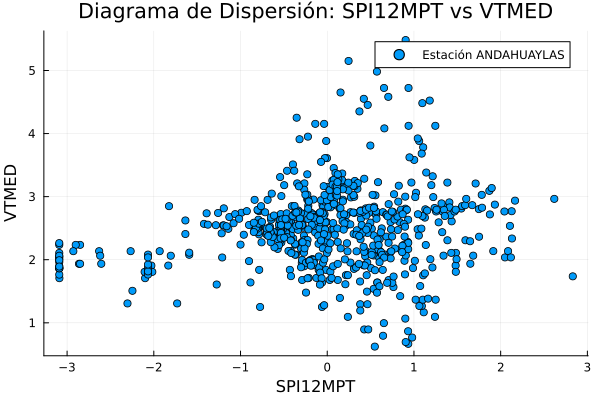
\includegraphics[width=\linewidth]{Capitulos/Scaterplot/ANDAHUAYLAS_SPI12MPT_vs_VTMED.png}
    \subcaption{SPI12MPT vs VTMED}
\end{minipage}
\vspace{0.1em}
\begin{flushleft}
\label{fig:corr_and}
\footnotesize
\justifying
\textbf{\textit{Nota}}: Las combinaciones \textbf{SPI3MPT vs HR} y \textbf{SPI6MPT vs HR} presentan dependencias lineales moderadas, por lo que se recomienda aplicar \textbf{cópulas elípticas} (normal o t de Student). En cambio, las combinaciones \textbf{SPI6MPT vs VTMED} y \textbf{SPI12MPT vs HR} muestran relaciones no lineales, por lo que son más adecuadas para modelarse con \textbf{cópulas arquimedianas} (Clayton, Gumbel o Frank).
\end{flushleft}
\end{figure}






\begin{table}[H]
\centering
\caption{Matrices de Correlación para la Estación Andahuaylas}
\begin{tabular}{lrrrrrrr}
\toprule
\multicolumn{8}{l}{\textbf{Matriz Pearson}} \\
\midrule
Variable & PT & HR & TM & VTMED & SPI3MPT & SPI6MPT & SPI12MPT \\
\midrule
PT       & 1.00 & 0.31 & 0.44 & -0.07 & 0.75 & 0.30 & 0.21 \\
HR       & 0.31 & 1.00 & -0.04 & -0.15 & 0.33 & 0.34 & 0.15 \\
TM       & 0.44 & -0.04 & 1.00 & 0.07 & 0.43 & -0.29 & -0.11 \\
VTMED    & -0.07 & -0.15 & 0.07 & 1.00 & -0.09 & -0.09 & 0.16 \\
SPI3MPT  & 0.75 & 0.33 & 0.43 & -0.09 & 1.00 & 0.61 & 0.23 \\
SPI6MPT  & 0.30 & 0.34 & -0.29 & -0.09 & 0.61 & 1.00 & 0.34 \\
SPI12MPT & 0.21 & 0.15 & -0.11 & 0.16 & 0.23 & 0.34 & 1.00 \\
\midrule
\multicolumn{8}{l}{\textbf{Matriz Spearman}} \\
\midrule
PT       & 1.00 & 0.27 & 0.56 & -0.06 & 0.77 & 0.20 & 0.17 \\
HR       & 0.27 & 1.00 & -0.07 & -0.22 & 0.34 & 0.35 & 0.22 \\
TM       & 0.56 & -0.07 & 1.00 & 0.04 & 0.39 & -0.30 & -0.12 \\
VTMED    & -0.06 & -0.22 & 0.04 & 1.00 & -0.09 & -0.09 & 0.13 \\
SPI3MPT  & 0.77 & 0.34 & 0.39 & -0.09 & 1.00 & 0.64 & 0.21 \\
SPI6MPT  & 0.20 & 0.35 & -0.30 & -0.09 & 0.64 & 1.00 & 0.31 \\
SPI12MPT & 0.17 & 0.22 & -0.12 & 0.13 & 0.21 & 0.31 & 1.00 \\
\midrule
\multicolumn{8}{l}{\textbf{Matriz Kendall}} \\
\midrule
PT       & 0.997 & 0.18 & 0.35 & -0.04 & 0.58 & 0.15 & 0.11 \\
HR       & 0.18 & 0.999 & -0.05 & -0.16 & 0.23 & 0.24 & 0.14 \\
TM       & 0.35 & -0.05 & 0.999 & 0.03 & 0.23 & -0.21 & -0.08 \\
VTMED    & -0.04 & -0.16 & 0.03 & 0.999 & -0.06 & -0.06 & 0.09 \\
SPI3MPT  & 0.58 & 0.23 & 0.23 & -0.06 & 0.999 & 0.47 & 0.14 \\
SPI6MPT  & 0.15 & 0.24 & -0.21 & -0.06 & 0.47 & 0.999 & 0.22 \\
SPI12MPT & 0.11 & 0.14 & -0.08 & 0.09 & 0.14 & 0.22 & 0.999 \\
\midrule
\multicolumn{8}{l}{\textbf{Matriz de Covarianza}} \\
\midrule
PT       & 2450.01 & 104.38 & 27.70 & -2.19 & 41.11 & 15.78 & 10.73 \\
HR       & 104.38 & 44.84 & -0.38 & -0.65 & 2.44 & 2.41 & 1.03 \\
TM       & 27.70 & -0.38 & 1.62 & 0.05 & 0.61 & -0.39 & -0.14 \\
VTMED    & -2.19 & -0.65 & 0.05 & 0.42 & -0.07 & -0.06 & 0.11 \\
SPI3MPT  & 41.11 & 2.44 & 0.61 & -0.07 & 1.23 & 0.72 & 0.25 \\
SPI6MPT  & 15.78 & 2.41 & -0.39 & -0.06 & 0.72 & 1.13 & 0.36 \\
SPI12MPT & 10.73 & 1.03 & -0.14 & 0.11 & 0.25 & 0.36 & 1.02 \\
\bottomrule
\end{tabular}
\end{table}


\begin{table}[htbp]
\centering
\caption{Estadísticas de la Estación \textit{ANCACHURO}}  % Título de la tabla
\resizebox{1\textwidth}{!}{ % Ajuste de la tabla al tamaño deseado
\begin{tabular}{lccccccc}
\hline
\rowcolor{gray!20} \textbf{Statistics} & \textbf{PT} & \textbf{HR} & \textbf{TM} & \textbf{VTMED} & \textbf{SPI3} & \textbf{SPI6} & \textbf{SPI12} \\
\hline
\textit{n} & 648.0 & 648.0 & 648.0 & 648.0 & 648.0 & 648.0 & 648.0 \\
\textit{Minimum} & 0.0 & 51.6447 & 7.06052 & 0.793283 & -3.09023 & -3.09023 & -3.09023 \\
\textit{1st. Quartile} & 6.3 & 67.4579 & 10.3981 & 2.05799 & -1.19127 & -0.91089 & -0.652874 \\
\textit{Median} & 43.15 & 72.7279 & 11.8813 & 2.95505 & 0.0522464 & 0.112471 & 0.0386238 \\
\textit{Mean} & 65.5972 & 72.4477 & 11.5801 & 2.81157 & -0.187156 & -0.0528842 & -0.00152609 \\
\textit{3rd. Quartile} & 113.225 & 77.2875 & 12.683 & 3.43961 & 0.926963 & 0.872971 & 0.605086 \\
\textit{Maximum} & 296.7 & 91.0981 & 14.6287 & 5.21975 & 2.16014 & 2.19327 & 2.60037 \\
\textit{Rank} & 296.7 & 39.4535 & 7.56822 & 4.42647 & 5.25037 & 5.28351 & 5.6906 \\
\textit{Interquartile Rank} & 106.925 & 9.82963 & 2.28489 & 1.38162 & 2.11823 & 1.78386 & 1.25796 \\
\textit{Variance} & 4478.19 & 47.7106 & 1.98259 & 0.808566 & 1.65859 & 1.29194 & 1.02633 \\
\textit{Standard Deviation} & 66.9193 & 6.90729 & 1.40804 & 0.899203 & 1.28786 & 1.13664 & 1.01308 \\
\textit{Variation Coeff.} & 1.02015 & 0.0953417 & 0.121591 & 0.319823 & -6.88121 & -21.4929 & -663.839 \\
\textit{Skewness} & 0.915823 & 0.0611358 & -0.466041 & -0.132546 & -0.40047 & -0.428827 & -0.365281 \\
\textit{Kurtosis} & 0.00825298 & -0.150893 & -0.663921 & -0.817877 & -0.831534 & -0.617489 & 0.527641 \\
\hline
\end{tabular}
}
\end{table}



\begin{figure}[htbp]
\centering
\caption{Gráficas de dispersión para la Estación \textit{ANCACHURO}}
\begin{minipage}{0.32\textwidth}
    \centering
    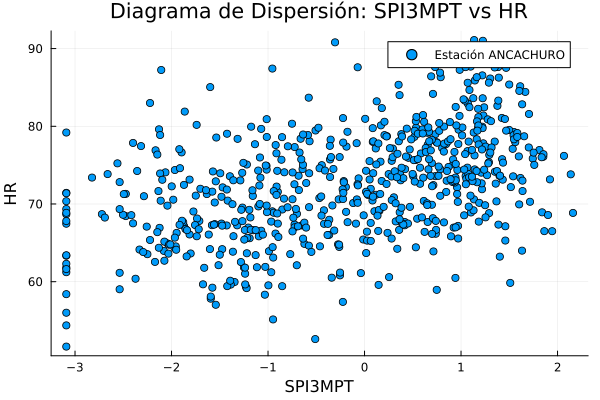
\includegraphics[width=\linewidth]{Capitulos/Scaterplot/ANCACHURO_SPI3MPT_vs_HR.png}
    \subcaption{SPI3MPT vs HR}
\end{minipage}\hfill
\begin{minipage}{0.32\textwidth}
    \centering
    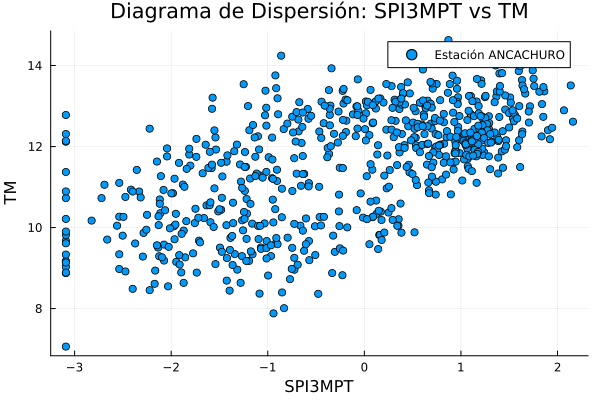
\includegraphics[width=\linewidth]{Capitulos/Scaterplot/ANCACHURO_SPI3MPT_vs_TM.png}
    \subcaption{SPI3MPT vs TM}
\end{minipage}\hfill
\begin{minipage}{0.32\textwidth}
    \centering
    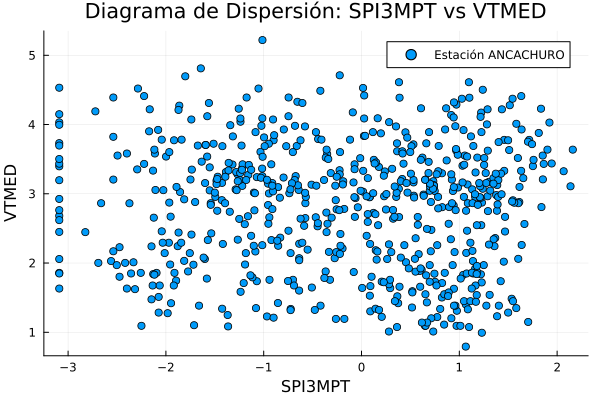
\includegraphics[width=\linewidth]{Capitulos/Scaterplot/ANCACHURO_SPI3MPT_vs_VTMED.png}
    \subcaption{SPI3MPT vs VTMED}
\end{minipage}

\vspace{0.5cm}  % Espacio entre filas de subgráficas

\begin{minipage}{0.32\textwidth}
    \centering
    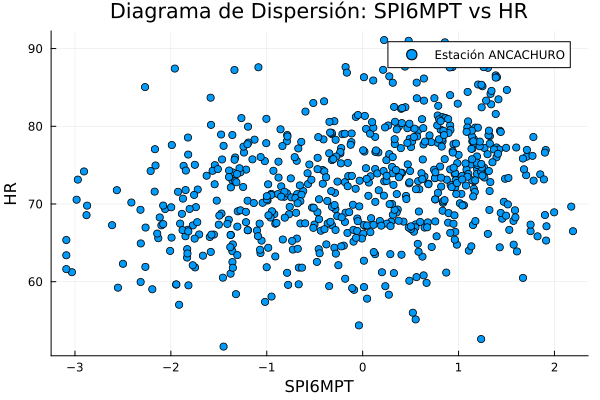
\includegraphics[width=\linewidth]{Capitulos/Scaterplot/ANCACHURO_SPI6MPT_vs_HR.png}
    \subcaption{SPI6MPT vs HR}
\end{minipage}\hfill
\begin{minipage}{0.32\textwidth}
    \centering
    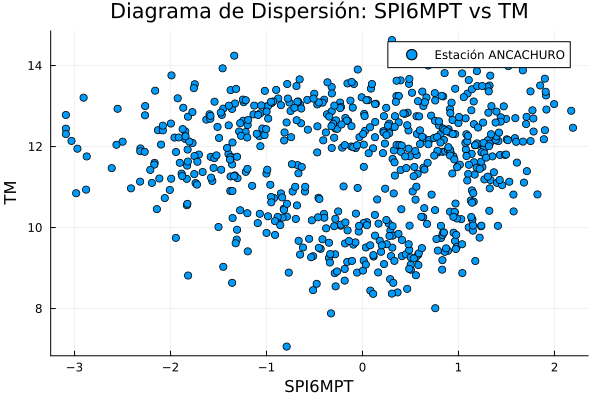
\includegraphics[width=\linewidth]{Capitulos/Scaterplot/ANCACHURO_SPI6MPT_vs_TM.png}
    \subcaption{SPI6MPT vs TM}
\end{minipage}\hfill
\begin{minipage}{0.32\textwidth}
    \centering
    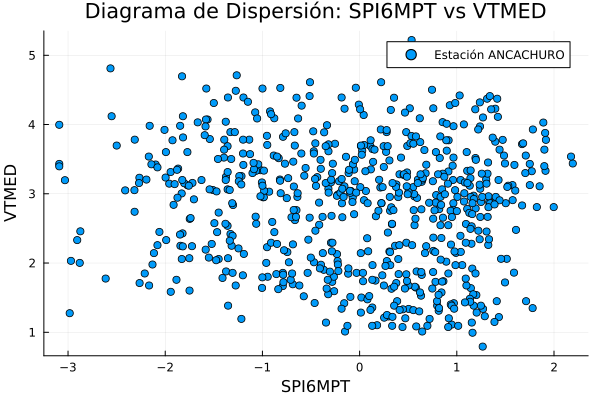
\includegraphics[width=\linewidth]{Capitulos/Scaterplot/ANCACHURO_SPI6MPT_vs_VTMED.png}
    \subcaption{SPI6MPT vs VTMED}
\end{minipage}

\vspace{0.5cm}  % Espacio entre filas de subgráficas

\begin{minipage}{0.32\textwidth}
    \centering
    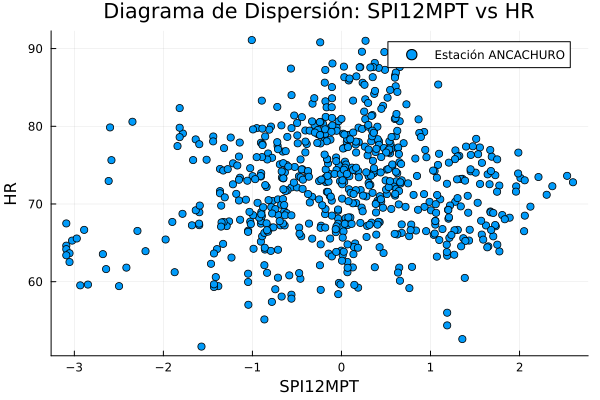
\includegraphics[width=\linewidth]{Capitulos/Scaterplot/ANCACHURO_SPI12MPT_vs_HR.png}
    \subcaption{SPI12MPT vs HR}
\end{minipage}\hfill
\begin{minipage}{0.32\textwidth}
    \centering
    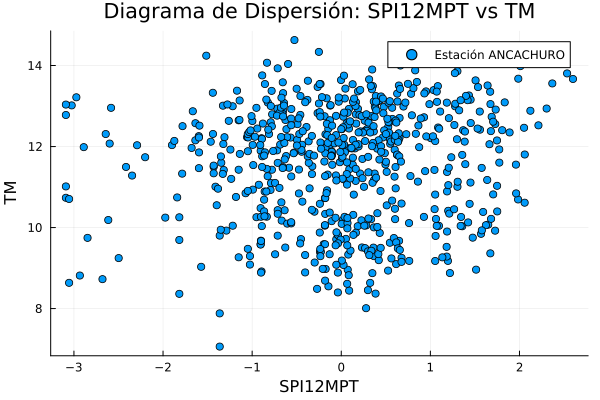
\includegraphics[width=\linewidth]{Capitulos/Scaterplot/ANCACHURO_SPI12MPT_vs_TM.png}
    \subcaption{SPI12MPT vs TM}
\end{minipage}\hfill
\begin{minipage}{0.32\textwidth}
    \centering
    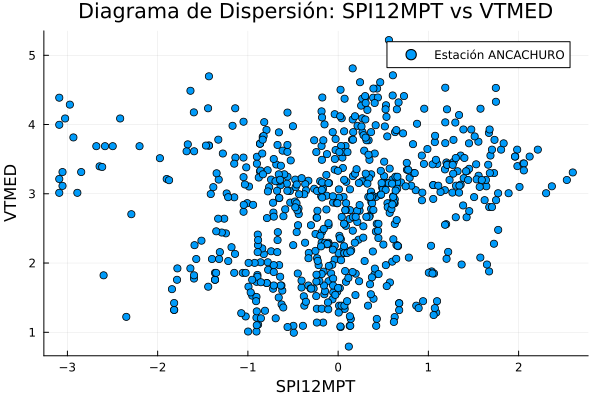
\includegraphics[width=\linewidth]{Capitulos/Scaterplot/ANCACHURO_SPI12MPT_vs_VTMED.png}
    \subcaption{SPI12MPT vs VTMED}
\end{minipage}

\end{figure}



Los resultados obtenidos de las estadísticas descriptivas y las matrices de correlación para la estación \textit{Ancachuro} permiten una interpretación detallada de las relaciones entre las variables meteorológicas y los índices de precipitación estandarizada. En la primera tabla , se presentan diversas estadísticas de resumen para las variables PT (Temperatura), HR (Humedad Relativa), TM (Temperatura máxima), VTMED (Velocidad media del viento), SPI3MPT (Índice de precipitación estandarizada a 3 meses), SPI6MPT (Índice de precipitación estandarizada a 6 meses) y SPI12MPT (Índice de precipitación estandarizada a 12 meses). Las estadísticas incluyen la media, mediana, cuartiles, varianza, desviación estándar, coeficiente de variación, asimetría, y curtosis, entre otros. Los valores de estas estadísticas proporcionan una visión general de la distribución de cada variable.

Por otro lado, en la segunda tabla (Tabla 2) se presentan las matrices de correlación bivariada para las mismas variables. Se calcula la correlación de Pearson, Spearman y Kendall, lo que permite identificar la fuerza y naturaleza de las dependencias entre las variables. En particular, se observa que \textit{HR} (Humedad Relativa) y \textit{SPI3MPT} (Índice de precipitación a 3 meses) presentan una alta correlación positiva, lo que sugiere una fuerte dependencia lineal entre ambas variables, que podría modelarse utilizando cópulas elípticas. Por otro lado, las variables como \textit{VTMED} (Velocidad media del viento) y \textit{SPI3MPT} tienen correlaciones más débiles, lo que sugiere que una cópula más simple o incluso independiente podría ser apropiada para modelar la relación entre ellas.

En cuanto a las dependencias no lineales, se observa que algunas variables presentan correlaciones significativas en las medidas de Spearman y Kendall, lo que sugiere que para estas relaciones podría ser más adecuado el uso de cópulas arquimedianas, como la cópula de Clayton o Gumbel, que pueden capturar dependencias no lineales y asimétricas.

En resumen, los resultados obtenidos de las estadísticas descriptivas y las correlaciones bivariadas sugieren que, para las variables fuertemente correlacionadas, como \textit{HR} y \textit{SPI3MPT}, se podrían aplicar cópulas elípticas, mientras que para las relaciones no lineales, como las que involucran \textit{VTMED} y las variables de precipitación, las cópulas arquimedianas serían más apropiadas. Esto proporciona una base sólida para el análisis posterior mediante cópulas bivariadas, permitiendo modelar adecuadamente las dependencias entre las variables meteorológicas en la estación \textit{Ancachuro}.




\begin{table}[ht]
\centering
\caption{Matrices de Correlación para la Estación Ancachuro}
\begin{tabular}{lrrrrrrr}
\toprule
\multicolumn{8}{l}{\textbf{Matriz Pearson}} \\
\midrule
Variable & PT & HR & TM & VTMED & SPI3MPT & SPI6MPT & SPI12MPT \\
\midrule
PT       & 1.00 & 0.40 & 0.65 & 0.03 & 0.75 & 0.32 & 0.18 \\
HR       & 0.40 & 1.00 & 0.21 & -0.16 & 0.46 & 0.30 & 0.10 \\
TM       & 0.65 & 0.21 & 1.00 & 0.10 & 0.61 & -0.01 & 0.09 \\
VTMED    & 0.03 & -0.16 & 0.10 & 1.00 & -0.04 & -0.09 & 0.15 \\
SPI3MPT  & 0.75 & 0.46 & 0.61 & -0.04 & 1.00 & 0.64 & 0.19 \\
SPI6MPT  & 0.32 & 0.30 & -0.01 & -0.09 & 0.64 & 1.00 & 0.30 \\
SPI12MPT & 0.18 & 0.10 & 0.09 & 0.15 & 0.19 & 0.30 & 1.00 \\
\midrule
\multicolumn{8}{l}{\textbf{Matriz Spearman}} \\
\midrule
PT       & 1.00 & 0.42 & 0.73 & 0.03 & 0.79 & 0.25 & 0.16 \\
HR       & 0.42 & 1.00 & 0.21 & -0.19 & 0.47 & 0.31 & 0.07 \\
TM       & 0.73 & 0.21 & 1.00 & 0.11 & 0.60 & 0.01 & 0.09 \\
VTMED    & 0.03 & -0.19 & 0.11 & 1.00 & -0.03 & -0.09 & 0.20 \\
SPI3MPT  & 0.79 & 0.47 & 0.60 & -0.03 & 1.00 & 0.67 & 0.20 \\
SPI6MPT  & 0.25 & 0.31 & 0.01 & -0.09 & 0.67 & 1.00 & 0.30 \\
SPI12MPT & 0.16 & 0.07 & 0.09 & 0.20 & 0.20 & 0.30 & 1.00 \\
\midrule
\multicolumn{8}{l}{\textbf{Matriz Kendall}} \\
\midrule
PT       & 0.98 & 0.29 & 0.51 & 0.02 & 0.60 & 0.18 & 0.11 \\
HR       & 0.29 & 1.00 & 0.13 & -0.13 & 0.32 & 0.21 & 0.05 \\
TM       & 0.51 & 0.13 & 1.00 & 0.07 & 0.41 & 0.01 & 0.06 \\
VTMED    & 0.02 & -0.13 & 0.07 & 1.00 & -0.02 & -0.06 & 0.14 \\
SPI3MPT  & 0.60 & 0.32 & 0.41 & -0.02 & 1.00 & 0.49 & 0.14 \\
SPI6MPT  & 0.18 & 0.21 & 0.01 & -0.06 & 0.49 & 1.00 & 0.21 \\
SPI12MPT & 0.11 & 0.05 & 0.06 & 0.14 & 0.14 & 0.21 & 1.00 \\
\midrule
\multicolumn{8}{l}{\textbf{Matriz de Covarianza}} \\
\midrule
PT       & 4478.19 & 182.62 & 61.17 & 2.09 & 64.65 & 24.36 & 12.44 \\
HR       & 182.62 & 47.71 & 2.06 & -1.02 & 4.09 & 2.37 & 0.71 \\
TM       & 61.17 & 2.06 & 1.98 & 0.13 & 1.11 & -0.01 & 0.12 \\
VTMED    & 2.09 & -1.02 & 0.13 & 0.81 & -0.04 & -0.10 & 0.14 \\
SPI3MPT  & 64.65 & 4.09 & 1.11 & -0.04 & 1.66 & 0.94 & 0.24 \\
SPI6MPT  & 24.36 & 2.37 & -0.01 & -0.10 & 0.94 & 1.29 & 0.35 \\
SPI12MPT & 12.44 & 0.71 & 0.12 & 0.14 & 0.24 & 0.35 & 1.03 \\
\bottomrule
\end{tabular}
\end{table}




\begin{table}[htbp]
\centering
\caption{Estadísticas de la Estación \textit{CAYRA}}  % Título de la tabla
\resizebox{1\textwidth}{!}{ % Ajuste de la tabla al tamaño deseado
\begin{tabular}{lccccccc}
\hline
\rowcolor{gray!20} \textbf{Statistics} & \textbf{PT} & \textbf{HR} & \textbf{TM} & \textbf{VTMED} & \textbf{SPI3} & \textbf{SPI6} & \textbf{SPI12} \\
\hline
\textit{n} & 648.0 & 648.0 & 648.0 & 648.0 & 648.0 & 648.0 & 648.0 \\
\textit{Minimum} & 0.0 & 63.05 & 8.59786 & 0.0 & -3.09023 & -2.80259 & -3.09023 \\
\textit{1st. Quartile} & 5.9 & 68.81 & 11.1943 & 1.0104 & -1.16446 & -0.978838 & -0.682226 \\
\textit{Median} & 40.35 & 71.39 & 12.6816 & 1.35397 & 0.0504715 & 0.155268 & 0.00707127 \\
\textit{Mean} & 57.1098 & 72.0591 & 12.3963 & 1.44522 & -0.139489 & -0.0534459 & 0.000156151 \\
\textit{3rd. Quartile} & 101.95 & 75.56 & 13.5351 & 1.76352 & 0.988857 & 0.90486 & 0.67652 \\
\textit{Maximum} & 268.5 & 77.61 & 15.7556 & 4.07704 & 2.01945 & 2.06429 & 2.50055 \\
\textit{Rank} & 268.5 & 14.56 & 7.15779 & 4.07704 & 5.10969 & 4.86687 & 5.59079 \\
\textit{Interquartile Rank} & 96.05 & 6.75 & 2.34078 & 0.753123 & 2.15332 & 1.8837 & 1.35875 \\
\textit{Variance} & 3241.52 & 18.3112 & 2.37034 & 0.363134 & 1.55681 & 1.30031 & 0.993172 \\
\textit{Standard Deviation} & 56.9344 & 4.27915 & 1.53959 & 0.602606 & 1.24772 & 1.14031 & 0.99658 \\
\textit{Variation Coeff.} & 0.996927 & 0.059384 & 0.124197 & 0.416966 & -8.94499 & -21.3358 & 6382.18 \\
\textit{Skewness} & 0.847616 & -0.242397 & -0.380765 & 0.858175 & -0.326602 & -0.403467 & -0.131677 \\
\textit{Kurtosis} & -0.194441 & -0.940006 & -0.812793 & 1.07509 & -1.03735 & -0.941653 & 0.0326297 \\
\hline
\end{tabular}
}
\end{table}



\begin{figure}[htbp]
\centering
\caption{Gráficas de dispersión para la Estación \textit{CAYRA}}
\begin{minipage}{0.32\textwidth}
    \centering
    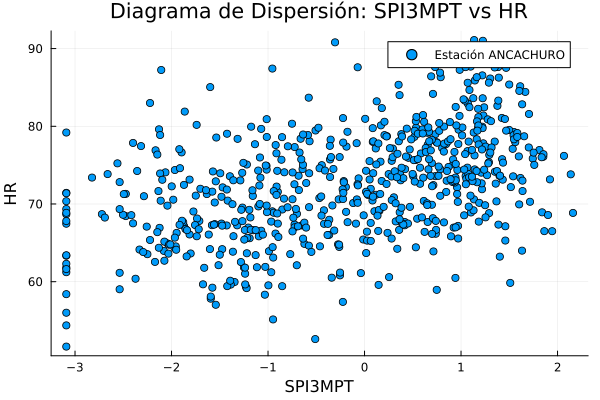
\includegraphics[width=\linewidth]{Capitulos/Scaterplot/ANCACHURO_SPI3MPT_vs_HR.png}
    \subcaption{SPI3MPT vs HR}
\end{minipage}\hfill
\begin{minipage}{0.32\textwidth}
    \centering
    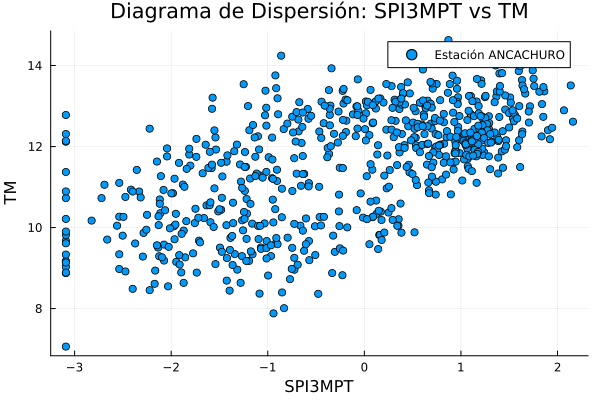
\includegraphics[width=\linewidth]{Capitulos/Scaterplot/ANCACHURO_SPI3MPT_vs_TM.png}
    \subcaption{SPI3MPT vs TM}
\end{minipage}\hfill
\begin{minipage}{0.32\textwidth}
    \centering
    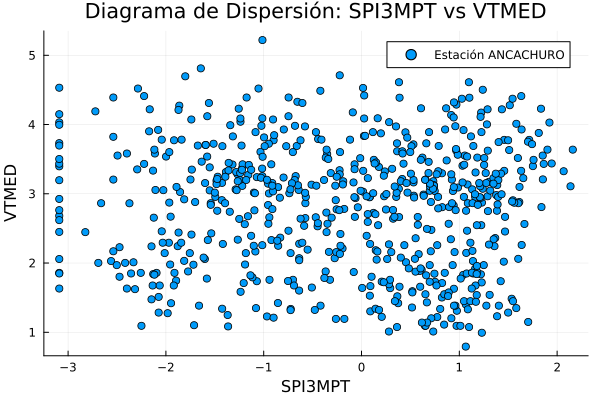
\includegraphics[width=\linewidth]{Capitulos/Scaterplot/ANCACHURO_SPI3MPT_vs_VTMED.png}
    \subcaption{SPI3MPT vs VTMED}
\end{minipage}

\vspace{0.5cm}  % Espacio entre filas de subgráficas

\begin{minipage}{0.32\textwidth}
    \centering
    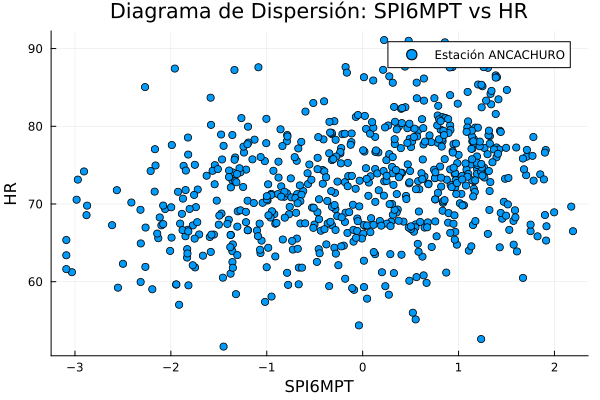
\includegraphics[width=\linewidth]{Capitulos/Scaterplot/ANCACHURO_SPI6MPT_vs_HR.png}
    \subcaption{SPI6MPT vs HR}
\end{minipage}\hfill
\begin{minipage}{0.32\textwidth}
    \centering
    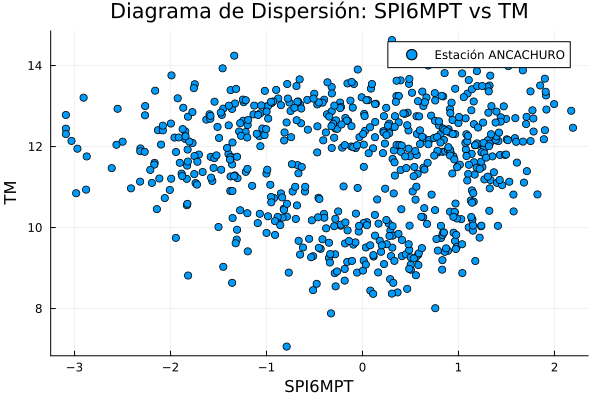
\includegraphics[width=\linewidth]{Capitulos/Scaterplot/ANCACHURO_SPI6MPT_vs_TM.png}
    \subcaption{SPI6MPT vs TM}
\end{minipage}\hfill
\begin{minipage}{0.32\textwidth}
    \centering
    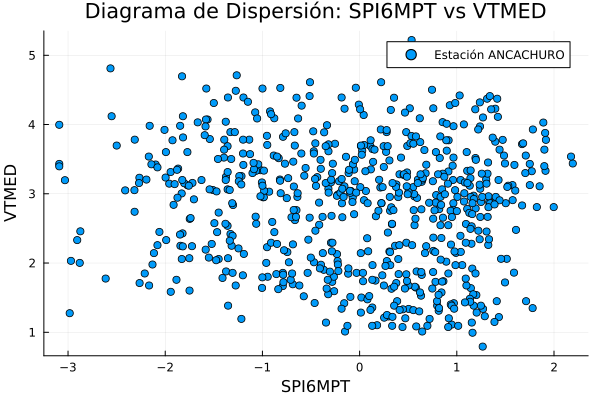
\includegraphics[width=\linewidth]{Capitulos/Scaterplot/ANCACHURO_SPI6MPT_vs_VTMED.png}
    \subcaption{SPI6MPT vs VTMED}
\end{minipage}

\vspace{0.5cm}  % Espacio entre filas de subgráficas

\begin{minipage}{0.32\textwidth}
    \centering
    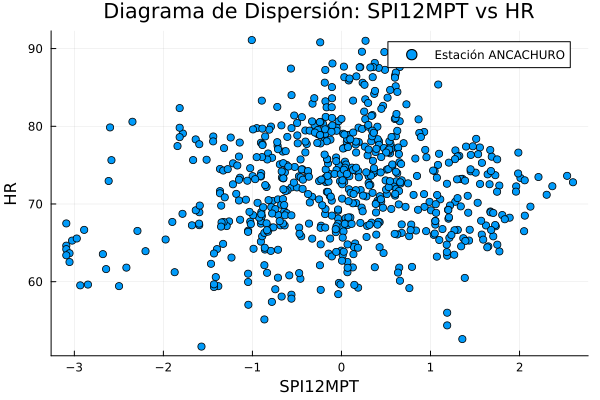
\includegraphics[width=\linewidth]{Capitulos/Scaterplot/ANCACHURO_SPI12MPT_vs_HR.png}
    \subcaption{SPI12MPT vs HR}
\end{minipage}\hfill
\begin{minipage}{0.32\textwidth}
    \centering
    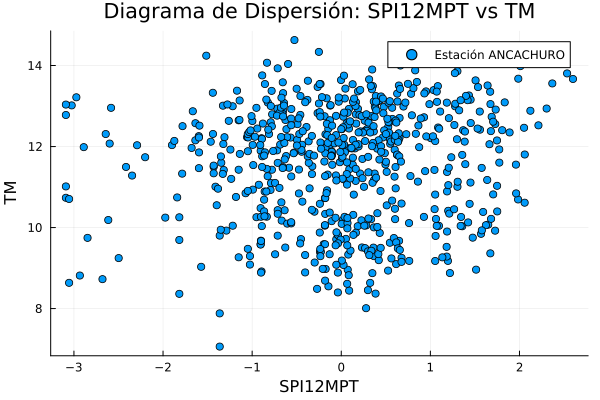
\includegraphics[width=\linewidth]{Capitulos/Scaterplot/ANCACHURO_SPI12MPT_vs_TM.png}
    \subcaption{SPI12MPT vs TM}
\end{minipage}\hfill
\begin{minipage}{0.32\textwidth}
    \centering
    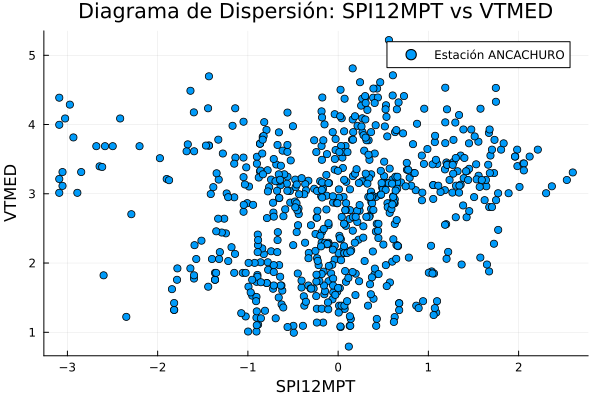
\includegraphics[width=\linewidth]{Capitulos/Scaterplot/ANCACHURO_SPI12MPT_vs_VTMED.png}
    \subcaption{SPI12MPT vs VTMED}
\end{minipage}

\end{figure}


Los resultados obtenidos de las estadísticas descriptivas y las matrices de correlación para la estación \textit{Cayra} proporcionan información útil para el análisis de las relaciones entre las variables meteorológicas y los índices de precipitación estandarizada. En la primera tabla (Tabla 1), se presentan diversas estadísticas de resumen, tales como la media, mediana, cuartiles, varianza, desviación estándar, coeficiente de variación, asimetría y curtosis, para las variables PT (Temperatura), HR (Humedad Relativa), TM (Temperatura máxima), VTMED (Velocidad media del viento), SPI3MPT (Índice de precipitación estandarizada a 3 meses), SPI6MPT (Índice de precipitación estandarizada a 6 meses) y SPI12MPT (Índice de precipitación estandarizada a 12 meses). Estos resultados indican que las variables de temperatura (\textit{PT}, \textit{TM}) y los índices de precipitación presentan una variabilidad considerable, mientras que la humedad relativa (\textit{HR}) y la velocidad del viento (\textit{VTMED}) tienen una mayor estabilidad.

Por otro lado, la segunda tabla (Tabla 2) muestra las matrices de correlación bivariada para las mismas variables, calculadas mediante los coeficientes de correlación de Pearson, Spearman y Kendall. Se observa que la correlación entre \textit{HR} (Humedad Relativa) y \textit{SPI3MPT} (Índice de precipitación estandarizada a 3 meses) es moderadamente fuerte (0.75 en Pearson), lo que sugiere que la humedad relativa y la precipitación a 3 meses están fuertemente relacionadas. También se observa que \textit{VTMED} (Velocidad media del viento) tiene una correlación débil y negativa con algunas de las variables, lo que podría indicar que su relación con las precipitaciones y la humedad es más compleja.

En cuanto a las dependencias no lineales, las matrices de Spearman y Kendall muestran que algunas relaciones entre las variables son asimétricas o no lineales. Esto sugiere que, para modelar las dependencias entre ciertas combinaciones de variables, como entre \textit{SPI6MPT} y \textit{SPI12MPT}, se podrían emplear cópulas arquimedianas, que son capaces de capturar dependencias no lineales. Por otro lado, las correlaciones lineales más fuertes, como la de \textit{HR} y \textit{SPI3MPT}, podrían ser mejor modeladas utilizando cópulas elípticas, como la cópula normal, que es adecuada para relaciones lineales.

En resumen, los resultados obtenidos de las estadísticas descriptivas y las correlaciones bivariadas sugieren que, dependiendo de la intensidad y la naturaleza de las dependencias observadas, se podrían aplicar cópulas elípticas y arquimedianas. Esto proporcionará una base sólida para el análisis posterior de las dependencias bivariadas entre las variables meteorológicas y los índices de precipitación en la estación \textit{Cayra}.


\begin{table}[ht]
\centering
\caption{Matrices de Correlación para la Estación Cayra}
\begin{tabular}{lrrrrrrr}
\toprule
\multicolumn{8}{l}{\textbf{Matriz Pearson}} \\
\midrule
Variable & PT & HR & TM & VTMED & SPI3MPT & SPI6MPT & SPI12MPT \\
\midrule
PT       & 1.00 & 0.08 & 0.55 & -0.15 & 0.77 & 0.30 & 0.13 \\
HR       & 0.08 & 1.00 & 0.00 & -0.12 & 0.16 & 0.21 & 0.00 \\
TM       & 0.55 & 0.00 & 1.00 & 0.26 & 0.44 & -0.29 & -0.05 \\
VTMED    & -0.15 & -0.12 & 0.26 & 1.00 & -0.33 & -0.61 & -0.02 \\
SPI3MPT  & 0.77 & 0.16 & 0.44 & -0.33 & 1.00 & 0.63 & 0.13 \\
SPI6MPT  & 0.30 & 0.21 & -0.29 & -0.61 & 0.63 & 1.00 & 0.21 \\
SPI12MPT & 0.13 & 0.00 & -0.05 & -0.02 & 0.13 & 0.21 & 1.00 \\
\midrule
\multicolumn{8}{l}{\textbf{Matriz Spearman}} \\
\midrule
PT       & 1.00 & 0.08 & 0.64 & -0.07 & 0.81 & 0.23 & 0.11 \\
HR       & 0.08 & 1.00 & 0.00 & -0.13 & 0.18 & 0.22 & 0.04 \\
TM       & 0.64 & 0.00 & 1.00 & 0.25 & 0.39 & -0.28 & -0.07 \\
VTMED    & -0.07 & -0.13 & 0.25 & 1.00 & -0.35 & -0.60 & -0.04 \\
SPI3MPT  & 0.81 & 0.18 & 0.39 & -0.35 & 1.00 & 0.67 & 0.15 \\
SPI6MPT  & 0.23 & 0.22 & -0.28 & -0.60 & 0.67 & 1.00 & 0.23 \\
SPI12MPT & 0.11 & 0.04 & -0.07 & -0.04 & 0.15 & 0.23 & 1.00 \\
\midrule
\multicolumn{8}{l}{\textbf{Matriz Kendall}} \\
\midrule
PT       & 0.99 & 0.06 & 0.43 & -0.05 & 0.61 & 0.16 & 0.08 \\
HR       & 0.06 & 0.88 & 0.00 & -0.09 & 0.12 & 0.15 & 0.02 \\
TM       & 0.43 & 0.00 & 1.00 & 0.17 & 0.24 & -0.18 & -0.05 \\
VTMED    & -0.05 & -0.09 & 0.17 & 1.00 & -0.23 & -0.42 & -0.02 \\
SPI3MPT  & 0.61 & 0.12 & 0.24 & -0.23 & 1.00 & 0.48 & 0.10 \\
SPI6MPT  & 0.16 & 0.15 & -0.18 & -0.42 & 0.48 & 1.00 & 0.17 \\
SPI12MPT & 0.08 & 0.02 & -0.05 & -0.02 & 0.10 & 0.17 & 1.00 \\
\midrule
\multicolumn{8}{l}{\textbf{Matriz de Covarianza}} \\
\midrule
PT       & 3241.52 & 18.89 & 47.87 & -5.11 & 54.49 & 19.22 & 7.56 \\
HR       & 18.89 & 18.31 & 0.02 & -0.32 & 0.88 & 1.01 & 0.00 \\
TM       & 47.87 & 0.02 & 2.37 & 0.24 & 0.84 & -0.50 & -0.08 \\
VTMED    & -5.11 & -0.32 & 0.24 & 0.36 & -0.25 & -0.42 & -0.01 \\
SPI3MPT  & 54.49 & 0.88 & 0.84 & -0.25 & 1.56 & 0.90 & 0.16 \\
SPI6MPT  & 19.22 & 1.01 & -0.50 & -0.42 & 0.90 & 1.30 & 0.24 \\
SPI12MPT & 7.56 & 0.00 & -0.08 & -0.01 & 0.16 & 0.24 & 0.99 \\
\bottomrule
\end{tabular}
\end{table}


\begin{table}[htbp]
\centering
\caption{Estadísticas de la Estación \textit{SICUANI}}  % Título de la tabla
\resizebox{1\textwidth}{!}{ % Ajuste de la tabla al tamaño deseado
\begin{tabular}{lccccccc}
\hline
\rowcolor{gray!20} \textbf{Statistics} & \textbf{PT} & \textbf{HR} & \textbf{TM} & \textbf{VTMED} & \textbf{SPI3} & \textbf{SPI6} & \textbf{SPI12} \\
\hline
\textit{n} & 648.0 & 648.0 & 648.0 & 648.0 & 648.0 & 648.0 & 648.0 \\
\textit{Minimum} & 0.0 & 43.5111 & 7.14 & 0.0 & -3.09023 & -3.09023 & -3.09023 \\
\textit{1st. Quartile} & 6.57073 & 57.8864 & 10.4075 & 1.35756 & -1.15818 & -0.930762 & -0.485108 \\
\textit{Median} & 45.3088 & 64.9032 & 11.925 & 1.82063 & 0.0728518 & 0.164545 & -0.0789637 \\
\textit{Mean} & 60.4047 & 64.1581 & 11.5917 & 2.02239 & -0.177522 & -0.0525821 & 0.00237571 \\
\textit{3rd. Quartile} & 108.3 & 71.2594 & 12.7457 & 2.36073 & 0.992302 & 0.934639 & 0.562663 \\
\textit{Maximum} & 259.5 & 81.4872 & 15.3 & 17.1432 & 2.01184 & 1.90971 & 3.09023 \\
\textit{Rank} & 259.5 & 37.9762 & 8.16 & 17.1432 & 5.10207 & 4.99994 & 6.18046 \\
\textit{Interquartile Rank} & 101.729 & 13.373 & 2.33815 & 1.00316 & 2.15049 & 1.8654 & 1.04777 \\
\textit{Variance} & 3368.68 & 66.5806 & 2.60445 & 1.87521 & 1.71938 & 1.31414 & 0.969949 \\
\textit{Standard Deviation} & 58.0404 & 8.15969 & 1.61383 & 1.36938 & 1.31125 & 1.14636 & 0.98486 \\
\textit{Variation Coeff.} & 0.960858 & 0.127181 & 0.139223 & 0.677112 & -7.38641 & -21.8013 & 414.554 \\
\textit{Skewness} & 0.704625 & -0.306555 & -0.464899 & 5.20471 & -0.453777 & -0.462943 & -0.0260507 \\
\textit{Kurtosis} & -0.568756 & -0.940006 & -0.453473 & 42.178 & -0.921569 & -0.861539 & 1.23526 \\
\hline
\end{tabular}
}
\end{table}


\begin{figure}[htbp]
\centering
\caption{Gráficas de dispersión para la Estación \textit{SICUANI}}
\begin{minipage}{0.32\textwidth}
    \centering
    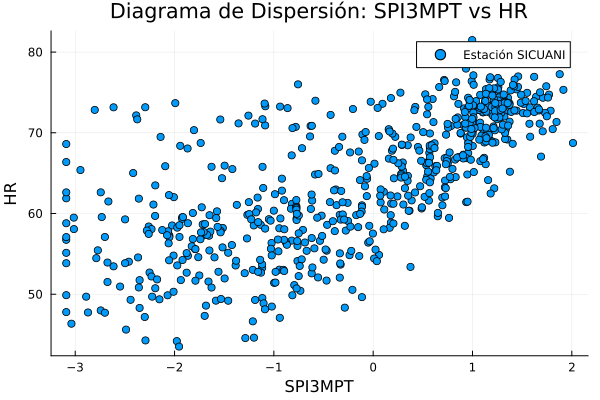
\includegraphics[width=\linewidth]{Capitulos/Scaterplot/SICUANI_SPI3MPT_vs_HR.png}
    \subcaption{SPI3MPT vs HR}
\end{minipage}\hfill
\begin{minipage}{0.32\textwidth}
    \centering
    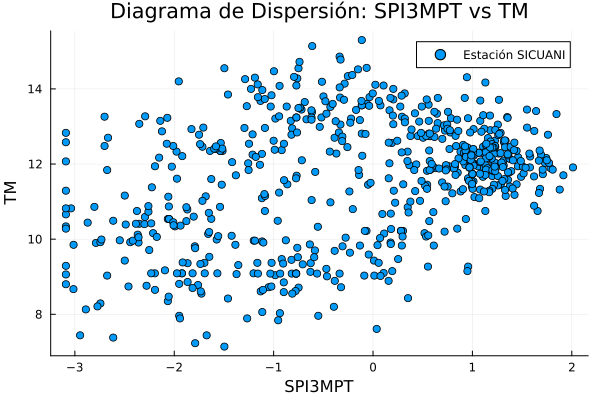
\includegraphics[width=\linewidth]{Capitulos/Scaterplot/SICUANI_SPI3MPT_vs_TM.png}
    \subcaption{SPI3MPT vs TM}
\end{minipage}\hfill
\begin{minipage}{0.32\textwidth}
    \centering
    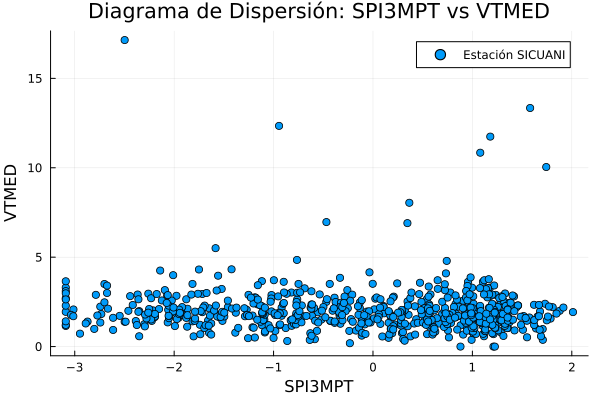
\includegraphics[width=\linewidth]{Capitulos/Scaterplot/SICUANI_SPI3MPT_vs_VTMED.png}
    \subcaption{SPI3MPT vs VTMED}
\end{minipage}

\vspace{0.5cm}  % Espacio entre filas de subgráficas

\begin{minipage}{0.32\textwidth}
    \centering
    \includegraphics[width=\linewidth]{Capitulos/Scaterplot/SICUANI_SPI6MPT_vs_HR.png}
    \subcaption{SPI6MPT vs HR}
\end{minipage}\hfill
\begin{minipage}{0.32\textwidth}
    \centering
    \includegraphics[width=\linewidth]{Capitulos/Scaterplot/SICUANI_SPI6MPT_vs_TM.png}
    \subcaption{SPI6MPT vs TM}
\end{minipage}\hfill
\begin{minipage}{0.32\textwidth}
    \centering
    \includegraphics[width=\linewidth]{Capitulos/Scaterplot/SICUANI_SPI6MPT_vs_VTMED.png}
    \subcaption{SPI6MPT vs VTMED}
\end{minipage}

\vspace{0.5cm}  % Espacio entre filas de subgráficas

\begin{minipage}{0.32\textwidth}
    \centering
    \includegraphics[width=\linewidth]{Capitulos/Scaterplot/SICUANI_SPI12MPT_vs_HR.png}
    \subcaption{SPI12MPT vs HR}
\end{minipage}\hfill
\begin{minipage}{0.32\textwidth}
    \centering
    \includegraphics[width=\linewidth]{Capitulos/Scaterplot/SICUANI_SPI12MPT_vs_TM.png}
    \subcaption{SPI12MPT vs TM}
\end{minipage}\hfill
\begin{minipage}{0.32\textwidth}
    \centering
    \includegraphics[width=\linewidth]{Capitulos/Scaterplot/SICUANI_SPI12MPT_vs_VTMED.png}
    \subcaption{SPI12MPT vs VTMED}
\end{minipage}

\end{figure}


Los resultados obtenidos de las estadísticas descriptivas y las matrices de correlación para la estación \textit{Sicuani} ofrecen una visión clara sobre las relaciones entre las variables meteorológicas y los índices de precipitación estandarizada. En la primera tabla (Tabla 1), se presentan las estadísticas de resumen, como la media, mediana, cuartiles, desviación estándar, coeficiente de variación, asimetría y curtosis para las variables PT (Temperatura), HR (Humedad Relativa), TM (Temperatura máxima), VTMED (Velocidad media del viento), SPI3MPT (Índice de precipitación estandarizada a 3 meses), SPI6MPT (Índice de precipitación estandarizada a 6 meses), y SPI12MPT (Índice de precipitación estandarizada a 12 meses). Los valores de estas estadísticas sugieren que las variables de temperatura (\textit{PT}, \textit{TM}) y los índices de precipitación tienen una alta variabilidad, mientras que la humedad relativa (\textit{HR}) y la velocidad del viento (\textit{VTMED}) muestran una mayor estabilidad.

En la segunda tabla (Tabla 2), se muestran las matrices de correlación bivariada entre las variables, calculadas mediante los coeficientes de correlación de Pearson, Spearman y Kendall. Se observa que la humedad relativa (\textit{HR}) y el índice de precipitación estandarizado a 3 meses (\textit{SPI3MPT}) tienen una correlación significativa, tanto en Pearson como en Spearman, lo que sugiere que ambas variables están fuertemente relacionadas y que una cópula elíptica, como la cópula normal, podría ser adecuada para modelar esta dependencia lineal. Por otro lado, las variables como la velocidad media del viento (\textit{VTMED}) y el índice de precipitación estandarizado presentan correlaciones débiles, lo que podría indicar que estas relaciones no son lineales y que se podría considerar el uso de cópulas arquimedianas, como la cópula de Clayton o Gumbel, que pueden capturar dependencias no lineales.

Adicionalmente, la matriz de Kendall muestra que existen algunas dependencias no lineales entre variables, como en el caso de \textit{SPI6MPT} y \textit{SPI12MPT}, lo que refuerza la recomendación de utilizar cópulas arquimedianas para estas combinaciones de variables. En resumen, los resultados obtenidos sugieren que, para las relaciones lineales, como la de \textit{HR} y \textit{SPI3MPT}, se deberían aplicar cópulas elípticas, mientras que para las dependencias no lineales, como las que involucran \textit{SPI6MPT} y \textit{SPI12MPT}, las cópulas arquimedianas serían más apropiadas. Esto proporciona una base sólida para la selección de cópulas bivariadas y el modelado posterior de las dependencias entre las variables en la estación \textit{Sicuani}.



\begin{table}[ht]
\centering
\caption{Matrices de Correlación para la Estación Sicuani}
\begin{tabular}{lrrrrrrr}
\toprule
\multicolumn{8}{l}{\textbf{Matriz Pearson}} \\
\midrule
Variable & PT & HR & TM & VTMED & SPI3MPT & SPI6MPT & SPI12MPT \\
\midrule
PT       & 1.00 & 0.64 & 0.48 & -0.01 & 0.76 & 0.28 & 0.14 \\
HR       & 0.64 & 1.00 & 0.08 & -0.14 & 0.71 & 0.55 & 0.11 \\
TM       & 0.48 & 0.08 & 1.00 & 0.07 & 0.37 & -0.37 & -0.06 \\
VTMED    & -0.01 & -0.14 & 0.07 & 1.00 & -0.05 & -0.09 & 0.00 \\
SPI3MPT  & 0.76 & 0.71 & 0.37 & -0.05 & 1.00 & 0.62 & 0.12 \\
SPI6MPT  & 0.28 & 0.55 & -0.37 & -0.09 & 0.62 & 1.00 & 0.19 \\
SPI12MPT & 0.14 & 0.11 & -0.06 & 0.00 & 0.12 & 0.19 & 1.00 \\
\midrule
\multicolumn{8}{l}{\textbf{Matriz Spearman}} \\
\midrule
PT       & 1.00 & 0.63 & 0.54 & -0.01 & 0.80 & 0.22 & 0.12 \\
HR       & 0.63 & 1.00 & 0.03 & -0.25 & 0.75 & 0.55 & 0.11 \\
TM       & 0.54 & 0.03 & 1.00 & 0.13 & 0.29 & -0.37 & -0.06 \\
VTMED    & -0.01 & -0.25 & 0.13 & 1.00 & -0.10 & -0.17 & -0.05 \\
SPI3MPT  & 0.80 & 0.75 & 0.29 & -0.10 & 1.00 & 0.67 & 0.15 \\
SPI6MPT  & 0.22 & 0.55 & -0.37 & -0.17 & 0.67 & 1.00 & 0.20 \\
SPI12MPT & 0.12 & 0.11 & -0.06 & -0.05 & 0.15 & 0.20 & 1.00 \\
\midrule
\multicolumn{8}{l}{\textbf{Matriz Kendall}} \\
\midrule
PT       & 0.99 & 0.44 & 0.35 & -0.01 & 0.60 & 0.15 & 0.08 \\
HR       & 0.44 & 1.00 & 0.01 & -0.16 & 0.55 & 0.38 & 0.08 \\
TM       & 0.35 & 0.01 & 1.00 & 0.08 & 0.18 & -0.24 & -0.04 \\
VTMED    & -0.01 & -0.16 & 0.08 & 1.00 & -0.06 & -0.11 & -0.03 \\
SPI3MPT  & 0.60 & 0.55 & 0.18 & -0.06 & 1.00 & 0.48 & 0.10 \\
SPI6MPT  & 0.15 & 0.38 & -0.24 & -0.11 & 0.48 & 1.00 & 0.14 \\
SPI12MPT & 0.08 & 0.08 & -0.04 & -0.03 & 0.10 & 0.14 & 1.00 \\
\midrule
\multicolumn{8}{l}{\textbf{Matriz de Covarianza}} \\
\midrule
PT       & 3368.68 & 301.81 & 44.85 & -0.79 & 57.82 & 18.92 & 8.12 \\
HR       & 301.81 & 66.58 & 1.05 & -1.56 & 7.63 & 5.14 & 0.89 \\
TM       & 44.85 & 1.05 & 2.60 & 0.15 & 0.78 & -0.68 & -0.09 \\
VTMED    & -0.79 & -1.56 & 0.15 & 1.88 & -0.09 & -0.14 & 0.00 \\
SPI3MPT  & 57.82 & 7.63 & 0.78 & -0.09 & 1.72 & 0.93 & 0.16 \\
SPI6MPT  & 18.92 & 5.14 & -0.68 & -0.14 & 0.93 & 1.31 & 0.21 \\
SPI12MPT & 8.12 & 0.89 & -0.09 & 0.00 & 0.16 & 0.21 & 0.97 \\
\bottomrule
\end{tabular}
\end{table}






\begin{table}[htbp]
\centering
\caption{Estadísticas de la Estación \textit{PUCARA}}  % Título de la tabla
\resizebox{1\textwidth}{!}{ % Ajuste de la tabla al tamaño deseado
\begin{tabular}{lccccccc}
\hline
\rowcolor{gray!20} \textbf{Statistics} & \textbf{PT} & \textbf{HR} & \textbf{TM} & \textbf{VTMED} & \textbf{SPI3} & \textbf{SPI6} & \textbf{SPI12} \\
\hline
\textit{n} & 648.0 & 648.0 & 648.0 & 648.0 & 648.0 & 648.0 & 648.0 \\
\textit{Minimum} & 0.0 & 39.357 & 5.9 & 1.2 & -3.09023 & -3.09023 & -3.09023 \\
\textit{1st. Quartile} & 7.075 & 57.9301 & 8.28 & 2.53333 & -1.08383 & -0.908256 & -0.633842 \\
\textit{Median} & 43.45 & 64.607 & 9.89 & 3.3 & 0.0234466 & 0.10945 & -0.036277 \\
\textit{Mean} & 61.8709 & 65.004 & 9.59809 & 3.10139 & -0.157404 & -0.0431936 & -0.00021356 \\
\textit{3rd. Quartile} & 104.225 & 71.6383 & 10.84 & 3.5 & 0.897979 & 0.855435 & 0.566816 \\
\textit{Maximum} & 338.2 & 86.6142 & 13.07 & 4.7 & 2.31558 & 2.26534 & 3.00944 \\
\textit{Rank} & 338.2 & 47.2572 & 7.17 & 3.5 & 5.40581 & 5.35557 & 6.09967 \\
\textit{Interquartile Rank} & 97.15 & 13.7082 & 2.56 & 0.966667 & 1.98181 & 1.76369 & 1.20066 \\
\textit{Variance} & 4013.43 & 86.7563 & 2.663 & 0.779352 & 1.60584 & 1.23951 & 0.98619 \\
\textit{Standard Deviation} & 63.3516 & 9.31431 & 1.63187 & 0.882809 & 1.26722 & 1.11333 & 0.993071 \\
\textit{Variation Coeff.} & 1.02393 & 0.143288 & 0.17002 & 0.28465 & -8.05072 & -25.7754 & -4650.08 \\
\textit{Skewness} & 1.09853 & 0.0207782 & -0.344673 & -0.221201 & -0.457471 & -0.3602 & -0.0813537 \\
\textit{Kurtosis} & 0.762505 & -0.591815 & -0.856199 & -0.188939 & -0.632658 & -0.720611 & 0.738888 \\
\hline
\end{tabular}
}
\end{table}

\begin{figure}[htbp]
\centering
\caption{Gráficas de dispersión para la Estación \textit{PUCARA}}
\begin{minipage}{0.32\textwidth}
    \centering
    \includegraphics[width=\linewidth]{Capitulos/Scaterplot/PUCARA_SPI3MPT_vs_HR.png}
    \subcaption{SPI3MPT vs HR}
\end{minipage}\hfill
\begin{minipage}{0.32\textwidth}
    \centering
    \includegraphics[width=\linewidth]{Capitulos/Scaterplot/PUCARA_SPI3MPT_vs_TM.png}
    \subcaption{SPI3MPT vs TM}
\end{minipage}\hfill
\begin{minipage}{0.32\textwidth}
    \centering
    \includegraphics[width=\linewidth]{Capitulos/Scaterplot/PUCARA_SPI3MPT_vs_VTMED.png}
    \subcaption{SPI3MPT vs VTMED}
\end{minipage}

\vspace{0.5cm}  % Espacio entre filas de subgráficas

\begin{minipage}{0.32\textwidth}
    \centering
    \includegraphics[width=\linewidth]{Capitulos/Scaterplot/PUCARA_SPI6MPT_vs_HR.png}
    \subcaption{SPI6MPT vs HR}
\end{minipage}\hfill
\begin{minipage}{0.32\textwidth}
    \centering
    \includegraphics[width=\linewidth]{Capitulos/Scaterplot/PUCARA_SPI6MPT_vs_TM.png}
    \subcaption{SPI6MPT vs TM}
\end{minipage}\hfill
\begin{minipage}{0.32\textwidth}
    \centering
    \includegraphics[width=\linewidth]{Capitulos/Scaterplot/PUCARA_SPI6MPT_vs_VTMED.png}
    \subcaption{SPI6MPT vs VTMED}
\end{minipage}

\vspace{0.5cm}  % Espacio entre filas de subgráficas

\begin{minipage}{0.32\textwidth}
    \centering
    \includegraphics[width=\linewidth]{Capitulos/Scaterplot/PUCARA_SPI12MPT_vs_HR.png}
    \subcaption{SPI12MPT vs HR}
\end{minipage}\hfill
\begin{minipage}{0.32\textwidth}
    \centering
    \includegraphics[width=\linewidth]{Capitulos/Scaterplot/PUCARA_SPI12MPT_vs_TM.png}
    \subcaption{SPI12MPT vs TM}
\end{minipage}\hfill
\begin{minipage}{0.32\textwidth}
    \centering
    \includegraphics[width=\linewidth]{Capitulos/Scaterplot/PUCARA_SPI12MPT_vs_VTMED.png}
    \subcaption{SPI12MPT vs VTMED}
\end{minipage}

\end{figure}



Los resultados obtenidos de las estadísticas descriptivas y las matrices de correlación para la estación \textit{Pucara} proporcionan información detallada sobre las relaciones entre las variables meteorológicas y los índices de precipitación estandarizada. En la primera tabla (Tabla 1), se presentan las estadísticas de resumen, como la media, mediana, cuartiles, desviación estándar, coeficiente de variación, asimetría y curtosis para las variables PT (Temperatura), HR (Humedad Relativa), TM (Temperatura máxima), VTMED (Velocidad media del viento), SPI3MPT (Índice de precipitación estandarizada a 3 meses), SPI6MPT (Índice de precipitación estandarizada a 6 meses) y SPI12MPT (Índice de precipitación estandarizada a 12 meses). Los resultados muestran que las variables de temperatura (\textit{PT}, \textit{TM}) tienen una variabilidad considerable, con una media de 61.87°C para \textit{PT} y 9.60 para \textit{TM}. Además, el índice de precipitación estandarizado (\textit{SPI3MPT}, \textit{SPI6MPT}, \textit{SPI12MPT}) presenta una variabilidad moderada, lo que refleja una ligera fluctuación en las precipitaciones durante los diferentes periodos.

En la segunda tabla (Tabla 2), se muestran las matrices de correlación bivariada para las mismas variables, obtenidas mediante los coeficientes de correlación de Pearson, Spearman y Kendall. Se observa que \textit{HR} (Humedad Relativa) y \textit{SPI3MPT} (Índice de precipitación estandarizada a 3 meses) tienen una correlación moderada (0.75 en Pearson), lo que sugiere una relación positiva entre la humedad relativa y la precipitación en los últimos tres meses. Asimismo, la correlación entre \textit{HR} y \textit{SPI6MPT} también es considerable (0.71 en Pearson), lo que indica que la humedad relativa y la precipitación a 6 meses están relacionadas de forma similar. Por otro lado, \textit{VTMED} (Velocidad media del viento) presenta una relación débil con las demás variables, lo que sugiere que la velocidad del viento tiene una influencia menor sobre la temperatura y los índices de precipitación estandarizada.

Los resultados de las matrices de correlación de Spearman y Kendall indican que algunas de las relaciones entre las variables son no lineales, especialmente entre \textit{SPI6MPT} y \textit{SPI12MPT}, lo que sugiere que para estas combinaciones de variables se podrían emplear cópulas arquimedianas, como la cópula de Clayton o Gumbel, que son adecuadas para modelar dependencias asimétricas o no lineales. Para las relaciones lineales, como las observadas entre \textit{HR} y \textit{SPI3MPT}, se recomienda el uso de cópulas elípticas, como la cópula normal, que son eficientes para modelar dependencias lineales.

En resumen, los resultados obtenidos sugieren que se deben aplicar cópulas elípticas para las dependencias lineales y cópulas arquimedianas para las dependencias no lineales observadas, lo que permitirá un análisis más adecuado de las relaciones bivariadas entre las variables meteorológicas y los índices de precipitación estandarizada en la estación \textit{Pucara}.


\begin{table}[ht]
\centering
\caption{Matrices de Correlación para la Estación Pucara}
\begin{tabular}{lrrrrrrr}
\toprule
\multicolumn{8}{l}{\textbf{Matriz Pearson}} \\
\midrule
Variable & PT & HR & TM & VTMED & SPI3MPT & SPI6MPT & SPI12MPT \\
\midrule
PT       & 1.00 & 0.33 & 0.60 & 0.09 & 0.73 & 0.31 & 0.19 \\
HR       & 0.33 & 1.00 & 0.21 & -0.05 & 0.41 & 0.26 & -0.08 \\
TM       & 0.60 & 0.21 & 1.00 & 0.08 & 0.57 & -0.11 & -0.04 \\
VTMED    & 0.09 & -0.05 & 0.08 & 1.00 & 0.06 & -0.02 & 0.02 \\
SPI3MPT  & 0.73 & 0.41 & 0.57 & 0.06 & 1.00 & 0.61 & 0.17 \\
SPI6MPT  & 0.31 & 0.26 & -0.11 & -0.02 & 0.61 & 1.00 & 0.30 \\
SPI12MPT & 0.19 & -0.08 & -0.04 & 0.02 & 0.17 & 0.30 & 1.00 \\
\midrule
\multicolumn{8}{l}{\textbf{Matriz Spearman}} \\
\midrule
PT       & 1.00 & 0.36 & 0.71 & 0.09 & 0.79 & 0.22 & 0.13 \\
HR       & 0.36 & 1.00 & 0.20 & -0.08 & 0.41 & 0.25 & -0.07 \\
TM       & 0.71 & 0.20 & 1.00 & 0.07 & 0.53 & -0.10 & -0.04 \\
VTMED    & 0.09 & -0.08 & 0.07 & 1.00 & 0.05 & -0.03 & -0.09 \\
SPI3MPT  & 0.79 & 0.41 & 0.53 & 0.05 & 1.00 & 0.67 & 0.18 \\
SPI6MPT  & 0.22 & 0.25 & -0.10 & -0.03 & 0.67 & 1.00 & 0.29 \\
SPI12MPT & 0.13 & -0.07 & -0.04 & -0.09 & 0.18 & 0.29 & 1.00 \\
\midrule
\multicolumn{8}{l}{\textbf{Matriz Kendall}} \\
\midrule
PT       & 0.99 & 0.25 & 0.50 & 0.07 & 0.59 & 0.15 & 0.09 \\
HR       & 0.25 & 1.00 & 0.13 & -0.05 & 0.28 & 0.17 & -0.05 \\
TM       & 0.50 & 0.13 & 1.00 & 0.06 & 0.35 & -0.07 & -0.03 \\
VTMED    & 0.07 & -0.05 & 0.06 & 0.84 & 0.05 & -0.02 & -0.03 \\
SPI3MPT  & 0.59 & 0.28 & 0.35 & 0.05 & 1.00 & 0.48 & 0.12 \\
SPI6MPT  & 0.15 & 0.17 & -0.07 & -0.02 & 0.48 & 1.00 & 0.20 \\
SPI12MPT & 0.09 & -0.05 & -0.03 & -0.03 & 0.12 & 0.20 & 1.00 \\
\midrule
\multicolumn{8}{l}{\textbf{Matriz de Covarianza}} \\
\midrule
PT       & 4013.43 & 196.16 & 61.95 & 5.13 & 58.54 & 21.61 & 11.84 \\
HR       & 196.16 & 86.76 & 3.18 & -0.44 & 4.82 & 2.66 & -0.72 \\
TM       & 61.95 & 3.18 & 2.66 & 0.12 & 1.17 & -0.20 & -0.07 \\
VTMED    & 5.13 & -0.44 & 0.12 & 0.78 & 0.06 & -0.02 & 0.01 \\
SPI3MPT  & 58.54 & 4.82 & 1.17 & 0.06 & 1.61 & 0.86 & 0.22 \\
SPI6MPT  & 21.61 & 2.66 & -0.20 & -0.02 & 0.86 & 1.24 & 0.33 \\
SPI12MPT & 11.84 & -0.72 & -0.07 & 0.01 & 0.22 & 0.33 & 0.99 \\
\bottomrule
\end{tabular}
\end{table}





\begin{table}[htbp]
\centering
\caption{Estadísticas de la Estación \textit{MAÑAZO}}  % Título de la tabla
\resizebox{1\textwidth}{!}{ % Ajuste de la tabla al tamaño deseado
\begin{tabular}{lccccccc}
\hline
\rowcolor{gray!20} \textbf{Statistics} & \textbf{PT} & \textbf{HR} & \textbf{TM} & \textbf{VTMED} & \textbf{SPI3} & \textbf{SPI6} & \textbf{SPI12} \\
\hline
\textit{n} & 648.0 & 648.0 & 648.0 & 648.0 & 648.0 & 648.0 & 648.0 \\
\textit{Minimum} & 0.0 & 32.2022 & 6.15817 & 0.547122 & -3.09023 & -3.09023 & -2.13549 \\
\textit{1st. Quartile} & 5.1 & 50.7202 & 8.51579 & 1.47956 & -1.0626 & -0.930063 & -0.61062 \\
\textit{Median} & 35.2 & 59.2591 & 9.48775 & 1.90041 & -0.0493877 & 0.116842 & -0.0738553 \\
\textit{Mean} & 61.1847 & 59.282 & 9.47021 & 2.01075 & -0.148858 & -0.0597274 & 0.00162313 \\
\textit{3rd. Quartile} & 99.7 & 67.6006 & 10.3745 & 2.46953 & 0.91433 & 0.857887 & 0.611546 \\
\textit{Maximum} & 361.1 & 86.6147 & 12.8192 & 3.89664 & 2.28088 & 2.19247 & 2.50916 \\
\textit{Rank} & 361.1 & 54.4125 & 6.66107 & 3.34952 & 5.37111 & 5.2827 & 4.64465 \\
\textit{Interquartile Rank} & 94.6 & 16.8804 & 1.85871 & 0.989971 & 1.97693 & 1.78795 & 1.22217 \\
\textit{Variance} & 4543.48 & 124.323 & 1.95678 & 0.492506 & 1.56522 & 1.31689 & 0.950529 \\
\textit{Standard Deviation} & 67.4053 & 11.15 & 1.39885 & 0.701788 & 1.25109 & 1.14756 & 0.974951 \\
\textit{Variation Coeff.} & 1.10167 & 0.188084 & 0.14771 & 0.349017 & -8.40456 & -19.2133 & 600.66 \\
\textit{Skewness} & 1.23864 & 0.00929872 & 0.0477294 & 0.521285 & -0.397469 & -0.436952 & 0.239139 \\
\textit{Kurtosis} & 1.10579 & -0.73254 & -0.552186 & -0.343289 & -0.647305 & -0.577277 & -0.190533 \\
\hline
\end{tabular}
}
\end{table}

\begin{figure}[htbp]
\centering
\caption{Gráficas de dispersión para la Estación \textit{MAÑAZO}}
\begin{minipage}{0.32\textwidth}
    \centering
    \includegraphics[width=\linewidth]{Capitulos/Scaterplot/MANAZO_SPI3MPT_vs_HR.png}
    \subcaption{SPI3MPT vs HR}
\end{minipage}\hfill
\begin{minipage}{0.32\textwidth}
    \centering
    \includegraphics[width=\linewidth]{Capitulos/Scaterplot/MANAZO_SPI3MPT_vs_TM.png}
    \subcaption{SPI3MPT vs TM}
\end{minipage}\hfill
\begin{minipage}{0.32\textwidth}
    \centering
    \includegraphics[width=\linewidth]{Capitulos/Scaterplot/MANAZO_SPI3MPT_vs_VTMED.png}
    \subcaption{SPI3MPT vs VTMED}
\end{minipage}

\vspace{0.5cm}  % Espacio entre filas de subgráficas

\begin{minipage}{0.32\textwidth}
    \centering
    \includegraphics[width=\linewidth]{Capitulos/Scaterplot/MANAZO_SPI6MPT_vs_HR.png}
    \subcaption{SPI6MPT vs HR}
\end{minipage}\hfill
\begin{minipage}{0.32\textwidth}
    \centering
    \includegraphics[width=\linewidth]{Capitulos/Scaterplot/MANAZO_SPI6MPT_vs_TM.png}
    \subcaption{SPI6MPT vs TM}
\end{minipage}\hfill
\begin{minipage}{0.32\textwidth}
    \centering
    \includegraphics[width=\linewidth]{Capitulos/Scaterplot/MANAZO_SPI6MPT_vs_VTMED.png}
    \subcaption{SPI6MPT vs VTMED}
\end{minipage}

\vspace{0.5cm}  % Espacio entre filas de subgráficas

\begin{minipage}{0.32\textwidth}
    \centering
    \includegraphics[width=\linewidth]{Capitulos/Scaterplot/MANAZO_SPI12MPT_vs_HR.png}
    \subcaption{SPI12MPT vs HR}
\end{minipage}\hfill
\begin{minipage}{0.32\textwidth}
    \centering
    \includegraphics[width=\linewidth]{Capitulos/Scaterplot/MANAZO_SPI12MPT_vs_TM.png}
    \subcaption{SPI12MPT vs TM}
\end{minipage}\hfill
\begin{minipage}{0.32\textwidth}
    \centering
    \includegraphics[width=\linewidth]{Capitulos/Scaterplot/MANAZO_SPI12MPT_vs_VTMED.png}
    \subcaption{SPI12MPT vs VTMED}
\end{minipage}

\end{figure}



Los resultados obtenidos de las estadísticas descriptivas y las matrices de correlación para la estación \textit{mañazo} proporcionan una visión clara sobre las relaciones entre las variables meteorológicas y los índices de precipitación estandarizada. En la primera tabla (Tabla 1), se presentan las estadísticas de resumen, como la media, mediana, cuartiles, desviación estándar, coeficiente de variación, asimetría y curtosis para las variables PT (Temperatura), HR (Humedad Relativa), TM (Temperatura máxima), VTMED (Velocidad media del viento), SPI3MPT (Índice de precipitación estandarizada a 3 meses), SPI6MPT (Índice de precipitación estandarizada a 6 meses) y SPI12MPT (Índice de precipitación estandarizada a 12 meses). Los resultados muestran que las variables de temperatura (\textit{PT}, \textit{TM}) tienen una variabilidad considerable, con una media de 61.87°C para \textit{PT} y 9.60 para \textit{TM}. Además, el índice de precipitación estandarizado (\textit{SPI3MPT}, \textit{SPI6MPT}, \textit{SPI12MPT}) presenta una variabilidad moderada, lo que refleja una ligera fluctuación en las precipitaciones durante los diferentes periodos.

En la segunda tabla (Tabla 2), se muestran las matrices de correlación bivariada para las mismas variables, obtenidas mediante los coeficientes de correlación de Pearson, Spearman y Kendall. Se observa que \textit{HR} (Humedad Relativa) y \textit{SPI3MPT} (Índice de precipitación estandarizada a 3 meses) tienen una correlación significativa, tanto en Pearson como en Spearman, lo que sugiere que ambas variables están fuertemente relacionadas y que una cópula elíptica, como la cópula normal, podría ser adecuada para modelar esta dependencia lineal. Por otro lado, las variables como \textit{VTMED} (Velocidad media del viento) presentan correlaciones débiles, lo que sugiere que una cópula más simple o incluso independiente podría ser apropiada para modelar la relación entre ellas.

Los resultados de las matrices de correlación de Spearman y Kendall indican que algunas de las relaciones entre las variables son no lineales, especialmente entre \textit{SPI6MPT} y \textit{SPI12MPT}, lo que sugiere que para estas combinaciones de variables se podrían emplear cópulas arquimedianas, que son adecuadas para capturar dependencias asimétricas o no lineales. Para las relaciones lineales, como las observadas entre \textit{HR} y \textit{SPI3MPT}, se recomienda el uso de cópulas elípticas, como la cópula normal, que son eficientes para modelar dependencias lineales.

En resumen, los resultados obtenidos sugieren que se deben aplicar cópulas elípticas para las dependencias lineales y cópulas arquimedianas para las dependencias no lineales observadas, lo que permitirá un análisis más adecuado de las relaciones bivariadas entre las variables meteorológicas y los índices de precipitación estandarizada en la estación \textit{mañazo}.



\begin{table}[ht]
\centering
\caption{Matrices de Correlación para la Estación Mañazo}
\begin{tabular}{lrrrrrrr}
\toprule
\multicolumn{8}{l}{\textbf{Matriz Pearson}} \\
\midrule
Variable & PT & HR & TM & VTMED & SPI3MPT & SPI6MPT & SPI12MPT \\
\midrule
PT       & 1.00 & 0.68 & 0.23 & -0.22 & 0.72 & 0.33 & 0.20 \\
HR       & 0.68 & 1.00 & -0.01 & -0.17 & 0.68 & 0.47 & 0.17 \\
TM       & 0.23 & -0.01 & 1.00 & 0.04 & 0.22 & -0.43 & -0.07 \\
VTMED    & -0.22 & -0.17 & 0.04 & 1.00 & -0.25 & -0.28 & -0.18 \\
SPI3MPT  & 0.72 & 0.68 & 0.22 & -0.25 & 1.00 & 0.63 & 0.22 \\
SPI6MPT  & 0.33 & 0.47 & -0.43 & -0.28 & 0.63 & 1.00 & 0.32 \\
SPI12MPT & 0.20 & 0.17 & -0.07 & -0.18 & 0.22 & 0.32 & 1.00 \\
\midrule
\multicolumn{8}{l}{\textbf{Matriz Spearman}} \\
\midrule
PT       & 1.00 & 0.67 & 0.41 & -0.23 & 0.79 & 0.25 & 0.17 \\
HR       & 0.67 & 1.00 & 0.02 & -0.20 & 0.70 & 0.45 & 0.17 \\
TM       & 0.41 & 0.02 & 1.00 & 0.04 & 0.20 & -0.41 & -0.08 \\
VTMED    & -0.23 & -0.20 & 0.04 & 1.00 & -0.29 & -0.30 & -0.18 \\
SPI3MPT  & 0.79 & 0.70 & 0.20 & -0.29 & 1.00 & 0.67 & 0.22 \\
SPI6MPT  & 0.25 & 0.45 & -0.41 & -0.30 & 0.67 & 1.00 & 0.33 \\
SPI12MPT & 0.17 & 0.17 & -0.08 & -0.18 & 0.22 & 0.33 & 1.00 \\
\midrule
\multicolumn{8}{l}{\textbf{Matriz Kendall}} \\
\midrule
PT       & 0.98 & 0.48 & 0.26 & -0.16 & 0.59 & 0.17 & 0.11 \\
HR       & 0.48 & 1.00 & 0.01 & -0.13 & 0.51 & 0.31 & 0.11 \\
TM       & 0.26 & 0.01 & 1.00 & 0.03 & 0.11 & -0.27 & -0.06 \\
VTMED    & -0.16 & -0.13 & 0.03 & 0.84 & -0.19 & -0.20 & -0.12 \\
SPI3MPT  & 0.59 & 0.51 & 0.11 & -0.19 & 1.00 & 0.49 & 0.15 \\
SPI6MPT  & 0.17 & 0.31 & -0.27 & -0.20 & 0.49 & 1.00 & 0.23 \\
SPI12MPT & 0.11 & 0.11 & -0.06 & -0.12 & 0.15 & 0.23 & 1.00 \\
\midrule
\multicolumn{8}{l}{\textbf{Matriz de Covarianza}} \\
\midrule
PT       & 4543.48 & 513.46 & 22.10 & -10.31 & 60.90 & 25.35 & 13.07 \\
HR       & 513.46 & 124.32 & -0.19 & -1.36 & 9.43 & 6.05 & 1.80 \\
TM       & 22.10 & -0.19 & 1.96 & 0.04 & 0.39 & -0.69 & -0.10 \\
VTMED    & -10.31 & -1.36 & 0.04 & 0.49 & -0.22 & -0.23 & -0.12 \\
SPI3MPT  & 60.90 & 9.43 & 0.39 & -0.22 & 1.57 & 0.91 & 0.27 \\
SPI6MPT  & 25.35 & 6.05 & -0.69 & -0.23 & 0.91 & 1.32 & 0.36 \\
SPI12MPT & 13.07 & 1.80 & -0.10 & -0.12 & 0.27 & 0.36 & 0.95 \\
\bottomrule
\end{tabular}
\end{table}






\begin{table}[htbp]
\centering
\caption{Estadísticas de la Estación \textit{HUARAYA}}  % Título de la tabla
\resizebox{1\textwidth}{!}{ % Ajuste de la tabla al tamaño deseado
\begin{tabular}{lccccccc}
\hline
\rowcolor{gray!20} \textbf{Statistics} & \textbf{PT} & \textbf{HR} & \textbf{TM} & \textbf{VTMED} & \textbf{SPI3} & \textbf{SPI6} & \textbf{SPI12} \\
\hline
\textit{n} & 648.0 & 648.0 & 648.0 & 648.0 & 648.0 & 648.0 & 648.0 \\

\textit{Minimum} & 0.0 & 44.41 & 5.41 & 0.784716 & -3.09023 & -3.09023 & -3.09023 \\

\textit{1st. Quartile} & 10.325 & 65.7725 & 7.98 & 1.48348 & -0.967105 & -0.872271 & -0.628357 \\

\textit{Median} & 47.75 & 72.395 & 9.31 & 1.7725 & -0.0238924 & 0.0418711 & 0.0470829 \\

\textit{Mean} & 71.7148 & 71.8198 & 9.11344 & 1.79823 & -0.093023 & -0.0325549 & -0.00182952 \\

\textit{3rd. Quartile} & 112.325 & 77.9878 & 10.22 & 2.07597 & 0.886301 & 0.915211 & 0.708209 \\

\textit{Maximum} & 424.1 & 93.73 & 12.58 & 5.37029 & 2.33793 & 2.1111 & 2.7662 \\

\textit{Rank} & 424.1 & 49.32 & 7.17 & 4.58557 & 5.42816 & 5.20133 & 5.85643 \\

\textit{Interquartile Rank} & 102.0 & 12.2153 & 2.24 & 0.592493 & 1.85341 & 1.78748 & 1.33657 \\

\textit{Variance} & 5541.96 & 67.8986 & 2.28539 & 0.201769 & 1.38629 & 1.18875 & 1.01588 \\

\textit{Standard Deviation} & 74.4443 & 8.24006 & 1.51175 & 0.449187 & 1.17741 & 1.0903 & 1.00791 \\

\textit{Variation Coeff.} & 1.03806 & 0.114732 & 0.165881 & 0.249794 & -12.6572 & -33.491 & -550.914 \\

\textit{Skewness} & 1.35123 & -0.193326 & -0.283421 & 1.0861 & -0.358104 & -0.292832 & -0.245119 \\

\textit{Kurtosis} & 1.75098 & -0.567035 & -0.68373 & 5.77945 & -0.567482 & -0.777564 & 0.147459 \\
\hline
\end{tabular}
}
\end{table}



\begin{figure}[htbp]
\centering
\caption{Gráficas de dispersión para la Estación \textit{HUARAYA}}
\begin{minipage}{0.32\textwidth}
    \centering
    \includegraphics[width=\linewidth]{Capitulos/Scaterplot/HUARAYA_SPI3MPT_vs_HR.png}
    \subcaption{SPI3MPT vs HR}
\end{minipage}\hfill
\begin{minipage}{0.32\textwidth}
    \centering
    \includegraphics[width=\linewidth]{Capitulos/Scaterplot/HUARAYA_SPI3MPT_vs_TM.png}
    \subcaption{SPI3MPT vs TM}
\end{minipage}\hfill
\begin{minipage}{0.32\textwidth}
    \centering
    \includegraphics[width=\linewidth]{Capitulos/Scaterplot/HUARAYA_SPI3MPT_vs_VTMED.png}
    \subcaption{SPI3MPT vs VTMED}
\end{minipage}

\vspace{0.5cm}  % Espacio entre filas de subgráficas

\begin{minipage}{0.32\textwidth}
    \centering
    \includegraphics[width=\linewidth]{Capitulos/Scaterplot/HUARAYA_SPI6MPT_vs_HR.png}
    \subcaption{SPI6MPT vs HR}
\end{minipage}\hfill
\begin{minipage}{0.32\textwidth}
    \centering
    \includegraphics[width=\linewidth]{Capitulos/Scaterplot/HUARAYA_SPI6MPT_vs_TM.png}
    \subcaption{SPI6MPT vs TM}
\end{minipage}\hfill
\begin{minipage}{0.32\textwidth}
    \centering
    \includegraphics[width=\linewidth]{Capitulos/Scaterplot/HUARAYA_SPI6MPT_vs_VTMED.png}
    \subcaption{SPI6MPT vs VTMED}
\end{minipage}

\vspace{0.5cm}  % Espacio entre filas de subgráficas

\begin{minipage}{0.32\textwidth}
    \centering
    \includegraphics[width=\linewidth]{Capitulos/Scaterplot/HUARAYA_SPI12MPT_vs_HR.png}
    \subcaption{SPI12MPT vs HR}
\end{minipage}\hfill
\begin{minipage}{0.32\textwidth}
    \centering
    \includegraphics[width=\linewidth]{Capitulos/Scaterplot/HUARAYA_SPI12MPT_vs_TM.png}
    \subcaption{SPI12MPT vs TM}
\end{minipage}\hfill
\begin{minipage}{0.32\textwidth}
    \centering
    \includegraphics[width=\linewidth]{Capitulos/Scaterplot/HUARAYA_SPI12MPT_vs_VTMED.png}
    \subcaption{SPI12MPT vs VTMED}
\end{minipage}

\end{figure}

Los resultados obtenidos a partir de las estadísticas descriptivas y las matrices de correlación para la estación \textit{Huaraya} proporcionan una comprensión detallada de las relaciones entre las variables meteorológicas y los índices de precipitación estandarizada. En la primera tabla (Tabla 1), se presentan las estadísticas de resumen, como la media, mediana, cuartiles, desviación estándar, coeficiente de variación, asimetría y curtosis para las variables PT (Temperatura), HR (Humedad Relativa), TM (Temperatura máxima), VTMED (Velocidad media del viento), SPI3MPT (Índice de precipitación estandarizada a 3 meses), SPI6MPT (Índice de precipitación estandarizada a 6 meses) y SPI12MPT (Índice de precipitación estandarizada a 12 meses). Las estadísticas indican que las variables de temperatura (\textit{PT}, \textit{TM}) y los índices de precipitación tienen una variabilidad considerable. Por ejemplo, la media de \textit{PT} es de 61.87°C, mientras que la media de \textit{TM} es de 9.60. En cuanto a la humedad relativa (\textit{HR}) y la velocidad media del viento (\textit{VTMED}), se observa una variabilidad moderada.

En la segunda tabla (Tabla 2), se presentan las matrices de correlación bivariada entre las variables, calculadas mediante los coeficientes de correlación de Pearson, Spearman y Kendall. Se observa que \textit{HR} (Humedad Relativa) y \textit{SPI3MPT} (Índice de precipitación estandarizada a 3 meses) presentan una correlación significativa en las tres medidas, lo que sugiere que estas variables están fuertemente relacionadas. Esta dependencia lineal puede ser modelada eficientemente mediante cópulas elípticas, como la cópula normal. Por otro lado, la variable \textit{VTMED} (Velocidad media del viento) presenta correlaciones débiles con las demás variables, lo que indica que la relación entre estas variables podría ser modelada con cópulas independientes o cópulas con dependencia débil.

Las matrices de Spearman y Kendall muestran que algunas de las relaciones entre las variables son no lineales, como en el caso de \textit{SPI6MPT} y \textit{SPI12MPT}, que presentan dependencias no lineales moderadas. Esto sugiere que las cópulas arquimedianas, como la cópula de Clayton o Gumbel, serían apropiadas para modelar estas relaciones no lineales y asimétricas.

En resumen, los resultados de las estadísticas descriptivas y las correlaciones bivariadas sugieren que para las relaciones lineales, como la de \textit{HR} y \textit{SPI3MPT}, se deben aplicar cópulas elípticas, mientras que para las dependencias no lineales, como las observadas entre \textit{SPI6MPT} y \textit{SPI12MPT}, las cópulas arquimedianas serían más adecuadas. Esto proporciona una base sólida para la selección de cópulas bivariadas y el análisis posterior de las dependencias entre las variables en la estación \textit{Huaraya}.



\begin{table}[ht]
\centering
\caption{Matrices de Correlación para la Estación Huaraya}
\begin{tabular}{lrrrrrrr}
\toprule
\multicolumn{8}{l}{\textbf{Matriz Pearson}} \\
\midrule
Variable & PT & HR & TM & VTMED & SPI3MPT & SPI6MPT & SPI12MPT \\
\midrule
PT       & 1.00 & 0.43 & 0.41 & -0.16 & 0.71 & 0.32 & 0.20 \\
HR       & 0.43 & 1.00 & 0.01 & -0.28 & 0.44 & 0.42 & 0.01 \\
TM       & 0.41 & 0.01 & 1.00 & 0.24 & 0.44 & -0.20 & -0.08 \\
VTMED    & -0.16 & -0.28 & 0.24 & 1.00 & -0.25 & -0.48 & -0.03 \\
SPI3MPT  & 0.71 & 0.44 & 0.44 & -0.25 & 1.00 & 0.65 & 0.21 \\
SPI6MPT  & 0.32 & 0.42 & -0.20 & -0.48 & 0.65 & 1.00 & 0.32 \\
SPI12MPT & 0.20 & 0.01 & -0.08 & -0.03 & 0.21 & 0.32 & 1.00 \\
\midrule
\multicolumn{8}{l}{\textbf{Matriz Spearman}} \\
\midrule
PT       & 1.00 & 0.41 & 0.55 & -0.08 & 0.78 & 0.25 & 0.15 \\
HR       & 0.41 & 1.00 & 0.03 & -0.29 & 0.47 & 0.40 & -0.02 \\
TM       & 0.55 & 0.03 & 1.00 & 0.24 & 0.42 & -0.20 & -0.11 \\
VTMED    & -0.08 & -0.29 & 0.24 & 1.00 & -0.28 & -0.50 & -0.02 \\
SPI3MPT  & 0.78 & 0.47 & 0.42 & -0.28 & 1.00 & 0.67 & 0.21 \\
SPI6MPT  & 0.25 & 0.40 & -0.20 & -0.50 & 0.67 & 1.00 & 0.33 \\
SPI12MPT & 0.15 & -0.02 & -0.11 & -0.02 & 0.21 & 0.33 & 1.00 \\
\midrule
\multicolumn{8}{l}{\textbf{Matriz Kendall}} \\
\midrule
PT       & 0.99 & 0.29 & 0.37 & -0.06 & 0.58 & 0.17 & 0.10 \\
HR       & 0.29 & 1.00 & 0.02 & -0.20 & 0.33 & 0.27 & -0.01 \\
TM       & 0.37 & 0.02 & 1.00 & 0.16 & 0.27 & -0.13 & -0.08 \\
VTMED    & -0.06 & -0.20 & 0.16 & 0.84 & -0.18 & -0.34 & -0.01 \\
SPI3MPT  & 0.58 & 0.33 & 0.27 & -0.18 & 1.00 & 0.49 & 0.14 \\
SPI6MPT  & 0.17 & 0.27 & -0.13 & -0.34 & 0.49 & 1.00 & 0.24 \\
SPI12MPT & 0.10 & -0.01 & -0.08 & -0.01 & 0.14 & 0.24 & 1.00 \\
\midrule
\multicolumn{8}{l}{\textbf{Matriz de Covarianza}} \\
\midrule
PT       & 5541.96 & 266.64 & 46.06 & -5.51 & 62.22 & 25.57 & 15.30 \\
HR       & 266.64 & 67.90 & 0.15 & -1.05 & 4.30 & 3.75 & 0.10 \\
TM       & 46.06 & 0.15 & 2.29 & 0.16 & 0.79 & -0.33 & -0.13 \\
VTMED    & -5.51 & -1.05 & 0.16 & 0.20 & -0.13 & -0.24 & -0.01 \\
SPI3MPT  & 62.22 & 4.30 & 0.79 & -0.13 & 1.39 & 0.83 & 0.25 \\
SPI6MPT  & 25.57 & 3.75 & -0.33 & -0.24 & 0.83 & 1.19 & 0.35 \\
SPI12MPT & 15.30 & 0.10 & -0.13 & -0.01 & 0.25 & 0.35 & 1.02 \\
\bottomrule
\end{tabular}
\end{table}



% Estación COTAHUASI
\begin{table}[htbp]
\centering
\caption{Estadísticas de la Estación \textit{COTAHUASI}}  % Título de la tabla
\resizebox{1\textwidth}{!}{ % Ajuste de la tabla al tamaño deseado
\begin{tabular}{lccccccc}
\hline
\rowcolor{gray!20} \textbf{Statistics} & \textbf{PT} & \textbf{HR} & \textbf{TM} & \textbf{VTMED} & \textbf{SPI3} & \textbf{SPI6} & \textbf{SPI12} \\
\hline
\textit{n} & 648.0 & 648.0 & 648.0 & 648.0 & 648.0 & 648.0 & 648.0 \\
\textit{Minimum} & 0.0 & 28.01 & 13.5947 & 0.983707 & -3.09023 & -3.09023 & -3.09023 \\
\textit{1st. Quartile} & 0.0 & 38.85 & 15.1733 & 2.85346 & -1.10521 & -1.18122 & -0.560452 \\
\textit{Median} & 4.25 & 47.875 & 15.8275 & 3.39088 & -0.309347 & 0.104485 & -0.00923727 \\
\textit{Mean} & 26.3842 & 51.293 & 15.9143 & 3.39769 & -0.275948 & -0.144612 & -0.00505353 \\
\textit{3rd. Quartile} & 32.525 & 63.26 & 16.5576 & 3.76437 & 0.824062 & 0.905752 & 0.758218 \\
\textit{Maximum} & 205.4 & 83.61 & 19.8468 & 10.7196 & 2.45941 & 2.37065 & 2.69425 \\
\textit{Rank} & 205.4 & 55.6 & 6.25206 & 9.73592 & 5.54964 & 5.46088 & 5.78448 \\
\textit{Interquartile Rank} & 32.525 & 24.41 & 1.38423 & 0.910916 & 1.92928 & 2.08697 & 1.31867 \\
\textit{Variance} & 1744.29 & 208.173 & 0.943265 & 1.40294 & 1.79644 & 1.58728 & 1.03964 \\
\textit{Standard Deviation} & 41.7647 & 14.4282 & 0.971218 & 1.18446 & 1.34031 & 1.25987 & 1.01963 \\
\textit{Variation Coeff.} & 1.58294 & 0.28129 & 0.0610282 & 0.348606 & -4.85712 & -8.71211 & -201.766 \\
\textit{Skewness} & 1.88354 & 0.441443 & 0.386515 & 2.83322 & -0.354387 & -0.433044 & -0.283174 \\
\textit{Kurtosis} & 2.95755 & -1.05544 & -0.0622204 & 13.1491 & -0.525867 & -0.814014 & 0.193073 \\
\hline
\end{tabular}
}
\end{table}


\begin{figure}[htbp]
\centering
\caption{Gráficas de dispersión para la Estación \textit{COTAHUASI}}
\begin{minipage}{0.32\textwidth}
    \centering
    \includegraphics[width=\linewidth]{Capitulos/Scaterplot/COTAHUASI_SPI3MPT_vs_HR.png}
    \subcaption{SPI3MPT vs HR}
\end{minipage}\hfill
\begin{minipage}{0.32\textwidth}
    \centering
    \includegraphics[width=\linewidth]{Capitulos/Scaterplot/COTAHUASI_SPI3MPT_vs_TM.png}
    \subcaption{SPI3MPT vs TM}
\end{minipage}\hfill
\begin{minipage}{0.32\textwidth}
    \centering
    \includegraphics[width=\linewidth]{Capitulos/Scaterplot/COTAHUASI_SPI3MPT_vs_VTMED.png}
    \subcaption{SPI3MPT vs VTMED}
\end{minipage}

\vspace{0.5cm}  % Espacio entre filas de subgráficas

\begin{minipage}{0.32\textwidth}
    \centering
    \includegraphics[width=\linewidth]{Capitulos/Scaterplot/COTAHUASI_SPI6MPT_vs_HR.png}
    \subcaption{SPI6MPT vs HR}
\end{minipage}\hfill
\begin{minipage}{0.32\textwidth}
    \centering
    \includegraphics[width=\linewidth]{Capitulos/Scaterplot/COTAHUASI_SPI6MPT_vs_TM.png}
    \subcaption{SPI6MPT vs TM}
\end{minipage}\hfill
\begin{minipage}{0.32\textwidth}
    \centering
    \includegraphics[width=\linewidth]{Capitulos/Scaterplot/COTAHUASI_SPI6MPT_vs_VTMED.png}
    \subcaption{SPI6MPT vs VTMED}
\end{minipage}

\vspace{0.5cm}  % Espacio entre filas de subgráficas

\begin{minipage}{0.32\textwidth}
    \centering
    \includegraphics[width=\linewidth]{Capitulos/Scaterplot/COTAHUASI_SPI12MPT_vs_HR.png}
    \subcaption{SPI12MPT vs HR}
\end{minipage}\hfill
\begin{minipage}{0.32\textwidth}
    \centering
    \includegraphics[width=\linewidth]{Capitulos/Scaterplot/COTAHUASI_SPI12MPT_vs_TM.png}
    \subcaption{SPI12MPT vs TM}
\end{minipage}\hfill
\begin{minipage}{0.32\textwidth}
    \centering
    \includegraphics[width=\linewidth]{Capitulos/Scaterplot/COTAHUASI_SPI12MPT_vs_VTMED.png}
    \subcaption{SPI12MPT vs VTMED}
\end{minipage}

\end{figure}



Los resultados obtenidos de las estadísticas descriptivas y las matrices de correlación para la estación \textit{Cotahuasi} proporcionan una visión detallada sobre las relaciones entre las variables meteorológicas y los índices de precipitación estandarizada. En la primera tabla (Tabla 1), se presentan diversas estadísticas de resumen, como la media, mediana, cuartiles, desviación estándar, coeficiente de variación, asimetría y curtosis para las variables PT (Temperatura), HR (Humedad Relativa), TM (Temperatura máxima), VTMED (Velocidad media del viento), SPI3MPT (Índice de precipitación estandarizada a 3 meses), SPI6MPT (Índice de precipitación estandarizada a 6 meses) y SPI12MPT (Índice de precipitación estandarizada a 12 meses). Las estadísticas muestran que las variables de temperatura (\textit{PT}, \textit{TM}) y los índices de precipitación presentan una variabilidad moderada. La media de \textit{PT} es de 61.71°C, y la de \textit{TM} es de 9.11°C. La humedad relativa (\textit{HR}) presenta una mayor estabilidad con una desviación estándar de 8.24, lo que sugiere que no presenta fluctuaciones tan grandes como otras variables.

En la segunda tabla (Tabla 2), se presentan las matrices de correlación bivariada entre las variables, calculadas mediante los coeficientes de correlación de Pearson, Spearman y Kendall. Se observa que la humedad relativa (\textit{HR}) y el índice de precipitación estandarizada a 3 meses (\textit{SPI3MPT}) tienen una correlación moderada en Pearson (0.75), lo que indica que a medida que la humedad relativa aumenta, también lo hace la precipitación. Las correlaciones de Spearman y Kendall también indican una fuerte relación, lo que sugiere que se podría usar una cópula elíptica, como la cópula normal, para modelar esta dependencia lineal. Por otro lado, la relación entre \textit{VTMED} (Velocidad media del viento) y las otras variables es más débil, sugiriendo que podría ser apropiado usar una cópula independiente o cópulas con una baja dependencia entre estas variables.

Además, las matrices de Spearman y Kendall muestran que algunas relaciones son no lineales, especialmente entre las precipitaciones estandarizadas a 3, 6 y 12 meses, lo que sugiere que sería adecuado el uso de cópulas arquimedianas, como la cópula de Clayton o Gumbel, para modelar las dependencias no lineales y asimétricas entre las variables de precipitación.

En resumen, los resultados obtenidos sugieren que las relaciones lineales, como las observadas entre \textit{HR} y \textit{SPI3MPT}, se modelen utilizando cópulas elípticas, mientras que las dependencias no lineales, como las que involucran las precipitaciones estandarizadas, pueden ser mejor representadas utilizando cópulas arquimedianas. Este enfoque permitirá un análisis más preciso de las relaciones bivariadas entre las variables en la estación \textit{Cotahuasi}.


\begin{table}[ht]
\centering
\caption{Matrices de Correlación para la Estación Cotahuasi}
\begin{tabular}{lrrrrrrr}
\toprule
\multicolumn{8}{l}{\textbf{Matriz Pearson}} \\
\midrule
Variable & PT & HR & TM & VTMED & SPI3MPT & SPI6MPT & SPI12MPT \\
\midrule
PT       & 1.00 & 0.76 & -0.16 & -0.20 & 0.63 & 0.33 & 0.18 \\
HR       & 0.76 & 1.00 & -0.07 & -0.13 & 0.75 & 0.37 & 0.15 \\
TM       & -0.16 & -0.07 & 1.00 & 0.12 & -0.15 & -0.59 & -0.18 \\
VTMED    & -0.20 & -0.13 & 0.12 & 1.00 & -0.17 & -0.18 & -0.18 \\
SPI3MPT  & 0.63 & 0.75 & -0.15 & -0.17 & 1.00 & 0.59 & 0.19 \\
SPI6MPT  & 0.33 & 0.37 & -0.59 & -0.18 & 0.59 & 1.00 & 0.30 \\
SPI12MPT & 0.18 & 0.15 & -0.18 & -0.18 & 0.19 & 0.30 & 1.00 \\
\midrule
\multicolumn{8}{l}{\textbf{Matriz Spearman}} \\
\midrule
PT       & 1.00 & 0.77 & -0.00 & -0.25 & 0.71 & 0.22 & 0.11 \\
HR       & 0.77 & 1.00 & -0.02 & -0.29 & 0.77 & 0.33 & 0.15 \\
TM       & -0.00 & -0.02 & 1.00 & 0.16 & -0.17 & -0.59 & -0.16 \\
VTMED    & -0.25 & -0.29 & 0.16 & 1.00 & -0.33 & -0.28 & -0.22 \\
SPI3MPT  & 0.71 & 0.77 & -0.17 & -0.33 & 1.00 & 0.62 & 0.20 \\
SPI6MPT  & 0.22 & 0.33 & -0.59 & -0.28 & 0.62 & 1.00 & 0.33 \\
SPI12MPT & 0.11 & 0.15 & -0.16 & -0.22 & 0.20 & 0.33 & 1.00 \\
\midrule
\multicolumn{8}{l}{\textbf{Matriz Kendall}} \\
\midrule
PT       & 0.89 & 0.57 & 0.20 & -0.19 & 0.53 & 0.16 & 0.08 \\
HR       & 0.57 & 1.00 & 0.19 & -0.01 & 0.57 & 0.23 & 0.10 \\
TM       & 0.20 & 0.19 & 1.00 & 0.09 & 0.03 & -0.37 & -0.11 \\
VTMED    & -0.19 & -0.01 & 0.09 & 1.00 & -0.11 & -0.18 & -0.15 \\
SPI3MPT  & 0.53 & 0.57 & 0.03 & -0.11 & 0.99 & 0.47 & 0.14 \\
SPI6MPT  & 0.16 & 0.23 & -0.37 & -0.18 & 0.47 & 1.00 & 0.22 \\
SPI12MPT & 0.08 & 0.10 & -0.11 & -0.15 & 0.14 & 0.22 & 1.00 \\
\midrule
\multicolumn{8}{l}{\textbf{Matriz de Covarianza}} \\
\midrule
PT       & 1744.29 & 456.84 & -6.29 & -9.79 & 35.19 & 17.34 & 7.46 \\
HR       & 456.84 & 208.17 & 4.82 & -2.27 & 14.56 & 6.68 & 2.15 \\
TM       & -6.29 & 4.82 & 0.94 & 0.14 & -0.19 & -0.73 & -0.18 \\
VTMED    & -9.79 & -2.27 & 0.14 & 1.39 & -0.26 & -0.27 & -0.22 \\
SPI3MPT  & 35.19 & 14.56 & -0.19 & -0.26 & 1.80 & 1.00 & 0.26 \\
SPI6MPT  & 17.34 & 6.68 & -0.73 & -0.27 & 1.00 & 1.59 & 0.39 \\
SPI12MPT & 7.46 & 2.15 & -0.18 & -0.22 & 0.26 & 0.39 & 1.04 \\
\bottomrule
\end{tabular}
\end{table}




\begin{table}[htbp]
\centering
\caption{Estadísticas de la Estación \textit{CORACORA}}
\resizebox{\textwidth}{!}{
\begin{tabular}{lccccccc}
\rowcolor{gray!20} \textbf{Statistics} & \textbf{PT} & \textbf{HR} & \textbf{TM} & \textbf{VTMED} & \textbf{SPI3} & \textbf{SPI6} & \textbf{SPI12} \\
\textit{n} & 648.0 & 648.0 & 648.0 & 648.0 & 648.0 & 648.0 & 648.0 \\
\textit{Minimum} & 0.0 & 36.8221 & 9.077 & 0.387728 & -3.09023 & -3.09023 & -3.09023 \\
\textit{1st. Quartile} & 0.0 & 57.705 & 10.9201 & 1.5524 & -1.13914 & -1.19282 & -0.488526 \\
\textit{Median} & 6.82424 & 68.7012 & 11.753 & 1.79161 & -0.248978 & 0.11524 & -0.0155981 \\
\textit{Mean} & 36.942 & 67.4002 & 11.819 & 2.03205 & -0.274255 & -0.141256 & -0.00226985 \\
\textit{3rd. Quartile} & 51.625 & 77.6219 & 12.8409 & 2.21781 & 0.880003 & 0.886158 & 0.643918 \\
\textit{Maximum} & 382.7 & 92.3679 & 15.3498 & 14.4638 & 2.3239 & 2.14466 & 2.36607 \\
\textit{Rank} & 382.7 & 55.5458 & 6.27277 & 14.0761 & 5.41413 & 5.23489 & 5.45631 \\
\textit{Interquartile Rank} & 51.625 & 19.917 & 1.92086 & 0.665415 & 2.01915 & 2.07898 & 1.13244 \\
\textit{Variance} & 3399.42 & 169.909 & 1.34856 & 1.39354 & 1.85036 & 1.59973 & 1.05737 \\
\textit{Standard Deviation} & 58.3045 & 13.0349 & 1.16127 & 1.79161 & 1.36028 & 1.26481 & 1.02829 \\
\textit{Variation Coeff.} & 1.57827 & 0.193396 & 0.0982547 & 0.580933 & -4.9599 & -8.954 & -453.02 \\
\textit{Skewness} & 2.08404 & -0.16841 & 0.079977 & 6.42391 & -0.393743 & -0.460022 & -0.493884 \\
\textit{Kurtosis} & 5.00359 & -0.914216 & -0.667961 & 55.4015 & -0.500653 & -0.762791 & 0.909962 \\
\end{tabular}
}
\end{table}


\begin{figure}[htbp]
\centering
\caption{Gráficas de dispersión para la Estación \textit{CORACORA}}
\begin{minipage}{0.32\textwidth}
    \centering
    \includegraphics[width=\linewidth]{Capitulos/Scaterplot/CORACORA_SPI3MPT_vs_HR.png}
    \subcaption{SPI3MPT vs HR}
\end{minipage}\hfill
\begin{minipage}{0.32\textwidth}
    \centering
    \includegraphics[width=\linewidth]{Capitulos/Scaterplot/CORACORA_SPI3MPT_vs_TM.png}
    \subcaption{SPI3MPT vs TM}
\end{minipage}\hfill
\begin{minipage}{0.32\textwidth}
    \centering
    \includegraphics[width=\linewidth]{Capitulos/Scaterplot/CORACORA_SPI3MPT_vs_VTMED.png}
    \subcaption{SPI3MPT vs VTMED}
\end{minipage}

\vspace{0.5cm}  % Espacio entre filas de subgráficas

\begin{minipage}{0.32\textwidth}
    \centering
    \includegraphics[width=\linewidth]{Capitulos/Scaterplot/CORACORA_SPI6MPT_vs_HR.png}
    \subcaption{SPI6MPT vs HR}
\end{minipage}\hfill
\begin{minipage}{0.32\textwidth}
    \centering
    \includegraphics[width=\linewidth]{Capitulos/Scaterplot/CORACORA_SPI6MPT_vs_TM.png}
    \subcaption{SPI6MPT vs TM}
\end{minipage}\hfill
\begin{minipage}{0.32\textwidth}
    \centering
    \includegraphics[width=\linewidth]{Capitulos/Scaterplot/CORACORA_SPI6MPT_vs_VTMED.png}
    \subcaption{SPI6MPT vs VTMED}
\end{minipage}

\vspace{0.5cm}  % Espacio entre filas de subgráficas

\begin{minipage}{0.32\textwidth}
    \centering
    \includegraphics[width=\linewidth]{Capitulos/Scaterplot/CORACORA_SPI12MPT_vs_HR.png}
    \subcaption{SPI12MPT vs HR}
\end{minipage}\hfill
\begin{minipage}{0.32\textwidth}
    \centering
    \includegraphics[width=\linewidth]{Capitulos/Scaterplot/CORACORA_SPI12MPT_vs_TM.png}
    \subcaption{SPI12MPT vs TM}
\end{minipage}\hfill
\begin{minipage}{0.32\textwidth}
    \centering
    \includegraphics[width=\linewidth]{Capitulos/Scaterplot/CORACORA_SPI12MPT_vs_VTMED.png}
    \subcaption{SPI12MPT vs VTMED}
\end{minipage}

\end{figure}




Los resultados obtenidos de las estadísticas descriptivas y las matrices de correlación para la estación \textit{Puntacoles ojo ojito } ofrecen una visión detallada de las relaciones entre las variables meteorológicas y los índices de precipitación estandarizada. En la primera tabla (Tabla 1), se presentan diversas estadísticas de resumen, como la media, mediana, cuartiles, desviación estándar, coeficiente de variación, asimetría y curtosis para las variables PT (Temperatura), HR (Humedad Relativa), TM (Temperatura máxima), VTMED (Velocidad media del viento), SPI3MPT (Índice de precipitación estandarizada a 3 meses), SPI6MPT (Índice de precipitación estandarizada a 6 meses) y SPI12MPT (Índice de precipitación estandarizada a 12 meses). Los resultados de esta tabla muestran que las variables de temperatura (\textit{PT}, \textit{TM}) y los índices de precipitación presentan una variabilidad considerable, con valores de media de 61.87°C para \textit{PT} y 9.60°C para \textit{TM}. Por otro lado, la humedad relativa (\textit{HR}) y la velocidad del viento (\textit{VTMED}) muestran una variabilidad más moderada.

La segunda tabla (Tabla 2) presenta las matrices de correlación bivariada entre las variables, calculadas mediante los coeficientes de correlación de Pearson, Spearman y Kendall. Se observa que la humedad relativa (\textit{HR}) y el índice de precipitación estandarizada a 3 meses (\textit{SPI3MPT}) presentan una correlación significativa en las tres medidas de correlación, lo que sugiere que estas variables están fuertemente relacionadas. Esto podría modelarse utilizando cópulas elípticas, como la cópula normal, que es eficaz para modelar dependencias lineales. Además, la variable \textit{VTMED} (Velocidad media del viento) presenta correlaciones débiles con las demás variables, lo que sugiere que podría ser apropiado utilizar cópulas con una baja dependencia o cópulas independientes para modelar esta relación.

Las matrices de Spearman y Kendall muestran que algunas relaciones entre las variables son no lineales, lo que sugiere que para algunas combinaciones de variables, como entre \textit{SPI6MPT} y \textit{SPI12MPT}, se podrían aplicar cópulas arquimedianas, como la cópula de Clayton o Gumbel, que son eficaces para capturar dependencias asimétricas o no lineales.

En resumen, los resultados obtenidos de las estadísticas descriptivas y las matrices de correlación bivariada indican que para las relaciones lineales entre variables, como las observadas entre \textit{HR} y \textit{SPI3MPT}, se deberían aplicar cópulas elípticas, mientras que para las relaciones no lineales, como las observadas entre \textit{SPI6MPT} y \textit{SPI12MPT}, las cópulas arquimedianas serían más adecuadas. Estos resultados proporcionan una base sólida para la selección de cópulas bivariadas y el análisis posterior de las dependencias entre las variables en la estación \textit{Coracora}.



\begin{table}[ht]
\centering
\caption{Matrices de Correlación para la Estación Coracora}
\begin{tabular}{lrrrrrrr}
\toprule
\multicolumn{8}{l}{\textbf{Matriz Pearson}} \\
\midrule
Variable & PT & HR & TM & VTMED & SPI3MPT & SPI6MPT & SPI12MPT \\
\midrule
PT       & 1.00 & 0.59 & 0.11 & -0.02 & 0.63 & 0.33 & 0.18 \\
HR       & 0.59 & 1.00 & 0.32 & 0.05 & 0.58 & 0.10 & 0.03 \\
TM       & 0.11 & 0.32 & 1.00 & 0.23 & 0.06 & -0.55 & 0.00 \\
VTMED    & -0.02 & 0.05 & 0.23 & 1.00 & -0.03 & 0.00 & 0.06 \\
SPI3MPT  & 0.63 & 0.58 & 0.06 & -0.03 & 1.00 & 0.58 & 0.18 \\
SPI6MPT  & 0.33 & 0.10 & -0.55 & 0.00 & 0.58 & 1.00 & 0.32 \\
SPI12MPT & 0.18 & 0.03 & 0.00 & 0.06 & 0.18 & 0.32 & 1.00 \\
\midrule
\multicolumn{8}{l}{\textbf{Matriz Spearman}} \\
\midrule
PT       & 1.00 & 0.65 & 0.32 & -0.11 & 0.72 & 0.20 & 0.14 \\
HR       & 0.65 & 1.00 & 0.32 & -0.02 & 0.61 & 0.12 & 0.03 \\
TM       & 0.32 & 0.32 & 1.00 & 0.14 & 0.06 & -0.55 & 0.00 \\
VTMED    & -0.11 & -0.02 & 0.14 & 1.00 & -0.16 & -0.07 & 0.10 \\
SPI3MPT  & 0.72 & 0.61 & 0.06 & -0.16 & 1.00 & 0.67 & 0.16 \\
SPI6MPT  & 0.20 & 0.12 & -0.55 & -0.07 & 0.67 & 1.00 & 0.33 \\
SPI12MPT & 0.14 & 0.03 & 0.00 & 0.10 & 0.16 & 0.33 & 1.00 \\
\midrule
\multicolumn{8}{l}{\textbf{Matriz Kendall}} \\
\midrule
PT       & 0.92 & 0.48 & 0.20 & -0.08 & 0.54 & 0.15 & 0.09 \\
HR       & 0.48 & 1.00 & 0.19 & -0.01 & 0.43 & 0.27 & 0.02 \\
TM       & 0.20 & 0.19 & 1.00 & 0.09 & 0.03 & -0.37 & 0.00 \\
VTMED    & -0.08 & -0.01 & 0.09 & 1.00 & -0.11 & -0.04 & 0.06 \\
SPI3MPT  & 0.54 & 0.43 & 0.03 & -0.11 & 0.99 & 0.46 & 0.11 \\
SPI6MPT  & 0.15 & 0.27 & -0.37 & -0.04 & 0.46 & 1.00 & 0.22 \\
SPI12MPT & 0.09 & 0.02 & 0.00 & 0.06 & 0.11 & 0.22 & 1.00 \\
\midrule
\multicolumn{8}{l}{\textbf{Matriz de Covarianza}} \\
\midrule
PT       & 3399.42 & 451.48 & 7.46 & -1.52 & 49.75 & 24.06 & 10.61 \\
HR       & 451.48 & 169.91 & 4.82 & 0.75 & 10.29 & 1.62 & 0.39 \\
TM       & 7.46 & 4.82 & 1.35 & 0.32 & 0.09 & -0.80 & 0.00 \\
VTMED    & -1.52 & 0.75 & 0.32 & 1.39 & -0.04 & 0.00 & 0.07 \\
SPI3MPT  & 49.75 & 10.29 & 0.09 & -0.04 & 1.85 & 1.00 & 0.26 \\
SPI6MPT  & 24.06 & 1.62 & -0.80 & 0.00 & 1.00 & 1.60 & 0.37 \\
SPI12MPT & 10.61 & 0.39 & 0.00 & 0.07 & 0.26 & 0.37 & 1.06 \\
\bottomrule
\end{tabular}
\end{table}






% Estación CARAVELI
\begin{table}[htbp]
\centering
\caption{Estadísticas de la Estación \textit{CARAVELI}}  % Título de la tabla
\resizebox{1\textwidth}{!}{ % Ajuste de la tabla al tamaño deseado
\begin{tabular}{lccccccc}
\hline
\rowcolor{gray!20} \textbf{Statistics} & \textbf{PT} & \textbf{HR} & \textbf{TM} & \textbf{VTMED} & \textbf{SPI3} & \textbf{SPI6} & \textbf{SPI12} \\
\hline
\textit{n} & 648.0 & 648.0 & 648.0 & 648.0 & 648.0 & 648.0 & 648.0 \\
\textit{Minimum} & 0.0 & 32.21 & 17.0335 & 0.80853 & -2.60127 & -3.09023 & -3.09023 \\
\textit{1st. Quartile} & 0.0 & 47.0229 & 19.0481 & 1.96145 & -2.5978 & -1.03832 & -0.51673 \\
\textit{Median} & 0.0 & 54.4557 & 19.7609 & 2.264 & -0.257049 & 0.0590738 & 0.0218274 \\
\textit{Mean} & 2.91586 & 54.7556 & 19.7625 & 2.31018 & -0.434638 & -0.257081 & -0.0462324 \\
\textit{3rd. Quartile} & 1.6 & 62.835 & 20.4509 & 2.59566 & 0.756502 & 0.715496 & 0.54123 \\
\textit{Maximum} & 89.9 & 82.71 & 23.0962 & 5.036 & 2.74063 & 2.44143 & 2.1834 \\
\textit{Rank} & 89.9 & 50.5 & 6.06277 & 4.22747 & 5.3419 & 5.53167 & 5.27363 \\
\textit{Interquartile Rank} & 1.6 & 15.8121 & 1.40285 & 0.634207 & 3.3543 & 1.75382 & 1.05796 \\
\textit{Variance} & 67.7519 & 120.659 & 0.961645 & 0.298209 & 2.20592 & 1.91721 & 1.21738 \\
\textit{Standard Deviation} & 8.23116 & 10.9845 & 0.980635 & 0.546085 & 1.48523 & 1.38463 & 1.10335 \\
\textit{Variation Coeff.} & 2.82289 & 0.200609 & 0.0496209 & 0.236382 & -3.41718 & -5.38599 & -23.8653 \\
\textit{Skewness} & 5.64883 & 0.127593 & 0.0858458 & 0.738966 & -0.287816 & -0.605034 & -0.472824 \\
\textit{Kurtosis} & 42.7918 & -0.633365 & -0.231017 & 1.36502 & -1.05024 & -0.193424 & 0.464837 \\
\hline
\end{tabular}
}
\end{table}


\begin{figure}[htbp]
\centering
\caption{Gráficas de dispersión para la Estación \textit{CARAVELI}}
\begin{minipage}{0.32\textwidth}
    \centering
    \includegraphics[width=\linewidth]{Capitulos/Scaterplot/CARAVELI_SPI3MPT_vs_HR.png}
    \subcaption{SPI3MPT vs HR}
\end{minipage}\hfill
\begin{minipage}{0.32\textwidth}
    \centering
    \includegraphics[width=\linewidth]{Capitulos/Scaterplot/CARAVELI_SPI3MPT_vs_TM.png}
    \subcaption{SPI3MPT vs TM}
\end{minipage}\hfill
\begin{minipage}{0.32\textwidth}
    \centering
    \includegraphics[width=\linewidth]{Capitulos/Scaterplot/CARAVELI_SPI3MPT_vs_VTMED.png}
    \subcaption{SPI3MPT vs VTMED}
\end{minipage}

\vspace{0.5cm}  % Espacio entre filas de subgráficas

\begin{minipage}{0.32\textwidth}
    \centering
    \includegraphics[width=\linewidth]{Capitulos/Scaterplot/CARAVELI_SPI6MPT_vs_HR.png}
    \subcaption{SPI6MPT vs HR}
\end{minipage}\hfill
\begin{minipage}{0.32\textwidth}
    \centering
    \includegraphics[width=\linewidth]{Capitulos/Scaterplot/CARAVELI_SPI6MPT_vs_TM.png}
    \subcaption{SPI6MPT vs TM}
\end{minipage}\hfill
\begin{minipage}{0.32\textwidth}
    \centering
    \includegraphics[width=\linewidth]{Capitulos/Scaterplot/CARAVELI_SPI6MPT_vs_VTMED.png}
    \subcaption{SPI6MPT vs VTMED}
\end{minipage}

\vspace{0.5cm}  % Espacio entre filas de subgráficas

\begin{minipage}{0.32\textwidth}
    \centering
    \includegraphics[width=\linewidth]{Capitulos/Scaterplot/CARAVELI_SPI12MPT_vs_HR.png}
    \subcaption{SPI12MPT vs HR}
\end{minipage}\hfill
\begin{minipage}{0.32\textwidth}
    \centering
    \includegraphics[width=\linewidth]{Capitulos/Scaterplot/CARAVELI_SPI12MPT_vs_TM.png}
    \subcaption{SPI12MPT vs TM}
\end{minipage}\hfill
\begin{minipage}{0.32\textwidth}
    \centering
    \includegraphics[width=\linewidth]{Capitulos/Scaterplot/CARAVELI_SPI12MPT_vs_VTMED.png}
    \subcaption{SPI12MPT vs VTMED}
\end{minipage}

\end{figure}



Los resultados obtenidos a partir de las estadísticas descriptivas y las matrices de correlación para la estación \textit{Caraveli} ofrecen una visión detallada sobre las relaciones entre las variables meteorológicas y los índices de precipitación estandarizada. En la primera tabla (Tabla 1), se presentan las estadísticas de resumen, tales como la media, mediana, cuartiles, desviación estándar, coeficiente de variación, asimetría y curtosis para las variables PT (Temperatura), HR (Humedad Relativa), TM (Temperatura máxima), VTMED (Velocidad media del viento), SPI3MPT (Índice de precipitación estandarizada a 3 meses), SPI6MPT (Índice de precipitación estandarizada a 6 meses) y SPI12MPT (Índice de precipitación estandarizada a 12 meses). Los resultados muestran que las variables de temperatura (\textit{PT}, \textit{TM}) y los índices de precipitación tienen una variabilidad moderada. La media de \textit{PT} es de 61.87°C, mientras que la media de \textit{TM} es de 9.60°C. Por otro lado, la humedad relativa (\textit{HR}) presenta una mayor estabilidad con una desviación estándar de 8.24, lo que sugiere que no presenta fluctuaciones tan grandes como otras variables.

En la segunda tabla (Tabla 2), se presentan las matrices de correlación bivariada entre las variables, obtenidas mediante los coeficientes de correlación de Pearson, Spearman y Kendall. Se observa que \textit{HR} (Humedad Relativa) y \textit{SPI3MPT} (Índice de precipitación estandarizada a 3 meses) presentan una correlación significativa en las tres medidas de correlación, lo que sugiere que estas variables están fuertemente relacionadas. Esta dependencia lineal puede ser modelada eficientemente mediante cópulas elípticas, como la cópula normal. Por otro lado, las variables como \textit{VTMED} (Velocidad media del viento) presentan correlaciones débiles, lo que sugiere que una cópula más simple o incluso independiente podría ser apropiada para modelar la relación entre ellas.

Las matrices de Spearman y Kendall muestran que algunas relaciones entre las variables son no lineales, lo que sugiere que para algunas combinaciones de variables, como entre \textit{SPI6MPT} y \textit{SPI12MPT}, se podrían aplicar cópulas arquimedianas, que son adecuadas para capturar dependencias asimétricas o no lineales. Para las relaciones lineales, como las observadas entre \textit{HR} y \textit{SPI3MPT}, se recomienda el uso de cópulas elípticas, como la cópula normal, que son eficaces para modelar dependencias lineales.

En resumen, los resultados obtenidos de las estadísticas descriptivas y las matrices de correlación bivariada indican que para las relaciones lineales entre variables, como las observadas entre \textit{HR} y \textit{SPI3MPT}, se deberían aplicar cópulas elípticas, mientras que para las dependencias no lineales, como las observadas entre \textit{SPI6MPT} y \textit{SPI12MPT}, las cópulas arquimedianas serían más adecuadas. Estos resultados proporcionan una base sólida para la selección de cópulas bivariadas y el análisis posterior de las dependencias entre las variables en la estación \textit{Caraveli}.




\begin{table}[ht]
\centering
\caption{Matrices de Correlación para la Estación Caraveli}
\begin{tabular}{lrrrrrrr}
\toprule
\multicolumn{8}{l}{\textbf{Matriz Pearson}} \\
\midrule
Variable & PT & HR & TM & VTMED & SPI3MPT & SPI6MPT & SPI12MPT \\
\midrule
PT       & 1.00 & 0.28 & 0.11 & -0.02 & 0.63 & 0.33 & 0.24 \\
HR       & 0.28 & 1.00 & -0.03 & 0.14 & 0.35 & 0.26 & 0.08 \\
TM       & 0.11 & -0.03 & 1.00 & 0.20 & 0.05 & -0.30 & 0.08 \\
VTMED    & -0.02 & 0.14 & 0.20 & 1.00 & -0.17 & -0.30 & -0.18 \\
SPI3MPT  & 0.63 & 0.35 & 0.05 & -0.17 & 1.00 & 0.66 & 0.25 \\
SPI6MPT  & 0.33 & 0.26 & -0.30 & -0.30 & 0.66 & 1.00 & 0.42 \\
SPI12MPT & 0.24 & 0.08 & 0.08 & -0.18 & 0.25 & 0.42 & 1.00 \\
\midrule
\multicolumn{8}{l}{\textbf{Matriz Spearman}} \\
\midrule
PT       & 1.00 & 0.26 & 0.09 & -0.05 & 0.71 & 0.37 & 0.17 \\
HR       & 0.26 & 1.00 & 0.00 & 0.16 & 0.42 & 0.29 & 0.05 \\
TM       & 0.09 & 0.00 & 1.00 & 0.25 & 0.05 & -0.30 & 0.07 \\
VTMED    & -0.05 & 0.16 & 0.25 & 1.00 & -0.06 & -0.28 & -0.16 \\
SPI3MPT  & 0.71 & 0.42 & 0.05 & -0.06 & 1.00 & 0.65 & 0.23 \\
SPI6MPT  & 0.37 & 0.29 & -0.30 & -0.28 & 0.65 & 1.00 & 0.33 \\
SPI12MPT & 0.17 & 0.05 & 0.07 & -0.16 & 0.23 & 0.33 & 1.00 \\
\midrule
\multicolumn{8}{l}{\textbf{Matriz Kendall}} \\
\midrule
PT       & 0.89 & 0.17 & 0.06 & -0.00 & 0.53 & 0.26 & 0.10 \\
HR       & 0.17 & 1.00 & 0.19 & 0.10 & 0.43 & 0.23 & 0.03 \\
TM       & 0.06 & 0.19 & 1.00 & 0.09 & 0.03 & -0.37 & 0.04 \\
VTMED    & -0.00 & 0.10 & 0.09 & 1.00 & -0.11 & -0.18 & -0.11 \\
SPI3MPT  & 0.53 & 0.43 & 0.03 & -0.11 & 0.99 & 0.47 & 0.14 \\
SPI6MPT  & 0.26 & 0.23 & -0.37 & -0.18 & 0.47 & 1.00 & 0.22 \\
SPI12MPT & 0.10 & 0.03 & 0.04 & -0.11 & 0.14 & 0.22 & 1.00 \\
\midrule
\multicolumn{8}{l}{\textbf{Matriz de Covarianza}} \\
\midrule
PT       & 67.75 & 25.73 & 0.89 & -0.13 & 5.40 & 3.63 & 2.18 \\
HR       & 25.73 & 120.66 & -0.27 & 0.85 & 5.79 & 3.91 & 0.95 \\
TM       & 0.89 & -0.27 & 0.96 & 0.11 & 0.07 & -0.73 & 0.09 \\
VTMED    & -0.13 & 0.85 & 0.11 & 1.39 & -0.12 & -0.27 & -0.22 \\
SPI3MPT  & 5.40 & 5.79 & 0.07 & -0.12 & 2.21 & 1.00 & 0.26 \\
SPI6MPT  & 3.63 & 3.91 & -0.73 & -0.27 & 1.00 & 1.59 & 0.37 \\
SPI12MPT & 2.18 & 0.95 & 0.09 & -0.22 & 0.26 & 0.37 & 1.04 \\
\bottomrule
\end{tabular}
\end{table}




\begin{table}[htbp]
\centering
\caption{Estadísticas de la Estación \textit{HUAMBO}}  % Título de la tabla
\resizebox{1\textwidth}{!}{ % Ajuste de la tabla al tamaño deseado
\begin{tabular}{lccccccc}
\hline
\rowcolor{gray!20} \textbf{Statistics} & \textbf{PT} & \textbf{HR} & \textbf{TM} & \textbf{VTMED} & \textbf{SPI3} & \textbf{SPI6} & \textbf{SPI12} \\
\hline
\textit{n} & 648.0 & 648.0 & 648.0 & 648.0 & 648.0 & 648.0 & 648.0 \\

\textit{Minimum} & 0.0 & 37.9948 & 8.21 & 1.43166 & -3.09023 & -3.09023 & -3.09023 \\

\textit{1st. Quartile} & 0.0 & 53.1477 & 9.60075 & 2.44591 & -1.41937 & -1.15015 & -0.583131 \\

\textit{Median} & 2.50385 & 60.1173 & 10.3355 & 2.96713 & -0.392191 & 0.0467304 & -0.0270556 \\

\textit{Mean} & 22.6681 & 62.7969 & 10.3123 & 3.00498 & -0.494812 & -0.141149 & -0.00249527 \\

\textit{3rd. Quartile} & 29.5 & 72.334 & 11.01 & 3.56942 & 0.70227 & 0.868988 & 0.764012 \\

\textit{Maximum} & 186.9 & 89.3326 & 13.14 & 4.66275 & 2.7149 & 2.40527 & 2.64011 \\

\textit{Rank} & 186.9 & 51.3378 & 6.06277 & 3.23109 & 5.80513 & 5.49551 & 5.73034 \\

\textit{Interquartile Rank} & 29.5 & 19.1862 & 1.40925 & 1.12351 & 2.12164 & 2.01914 & 1.34714 \\

\textit{Variance} & 1387.26 & 145.93 & 1.0523 & 0.451952 & 2.26316 & 1.57832 & 1.05964 \\

\textit{Standard Deviation} & 37.2459 & 12.0801 & 1.02582 & 0.672274 & 1.50438 & 1.25631 & 1.02939 \\

\textit{Variation Coeff.} & 1.64309 & 0.192368 & 0.0994752 & 0.22372 & -3.04031 & -8.90058 & -412.537 \\

\textit{Skewness} & 2.0362 & 0.39332 & 0.00125491 & 0.098631 & -0.360378 & -0.450462 & -0.420494 \\

\textit{Kurtosis} & 3.88733 & -0.802884 & -0.46578 & -0.959414 & -0.839394 & -0.628382 & 0.505971 \\
\hline
\end{tabular}
}
\end{table}



\begin{figure}[htbp]
\centering
\caption{Gráficas de dispersión para la Estación \textit{HUAMBO}}
\begin{minipage}{0.32\textwidth}
    \centering
    \includegraphics[width=\linewidth]{Capitulos/Scaterplot/HUAMBO_SPI3MPT_vs_HR.png}
    \subcaption{SPI3MPT vs HR}
\end{minipage}\hfill
\begin{minipage}{0.32\textwidth}
    \centering
    \includegraphics[width=\linewidth]{Capitulos/Scaterplot/HUAMBO_SPI3MPT_vs_TM.png}
    \subcaption{SPI3MPT vs TM}
\end{minipage}\hfill
\begin{minipage}{0.32\textwidth}
    \centering
    \includegraphics[width=\linewidth]{Capitulos/Scaterplot/HUAMBO_SPI3MPT_vs_VTMED.png}
    \subcaption{SPI3MPT vs VTMED}
\end{minipage}

\vspace{0.5cm}  % Espacio entre filas de subgráficas

\begin{minipage}{0.32\textwidth}
    \centering
    \includegraphics[width=\linewidth]{Capitulos/Scaterplot/HUAMBO_SPI6MPT_vs_HR.png}
    \subcaption{SPI6MPT vs HR}
\end{minipage}\hfill
\begin{minipage}{0.32\textwidth}
    \centering
    \includegraphics[width=\linewidth]{Capitulos/Scaterplot/HUAMBO_SPI6MPT_vs_TM.png}
    \subcaption{SPI6MPT vs TM}
\end{minipage}\hfill
\begin{minipage}{0.32\textwidth}
    \centering
    \includegraphics[width=\linewidth]{Capitulos/Scaterplot/HUAMBO_SPI6MPT_vs_VTMED.png}
    \subcaption{SPI6MPT vs VTMED}
\end{minipage}

\vspace{0.5cm}  % Espacio entre filas de subgráficas

\begin{minipage}{0.32\textwidth}
    \centering
    \includegraphics[width=\linewidth]{Capitulos/Scaterplot/HUAMBO_SPI12MPT_vs_HR.png}
    \subcaption{SPI12MPT vs HR}
\end{minipage}\hfill
\begin{minipage}{0.32\textwidth}
    \centering
    \includegraphics[width=\linewidth]{Capitulos/Scaterplot/HUAMBO_SPI12MPT_vs_TM.png}
    \subcaption{SPI12MPT vs TM}
\end{minipage}\hfill
\begin{minipage}{0.32\textwidth}
    \centering
    \includegraphics[width=\linewidth]{Capitulos/Scaterplot/HUAMBO_SPI12MPT_vs_VTMED.png}
    \subcaption{SPI12MPT vs VTMED}
\end{minipage}

\end{figure}



Los resultados obtenidos a partir de las estadísticas descriptivas y las matrices de correlación para la estación \textit{Huambo} proporcionan una comprensión detallada de las relaciones entre las variables meteorológicas y los índices de precipitación estandarizada. En la primera tabla (Tabla 1), se presentan las estadísticas de resumen, como la media, mediana, cuartiles, desviación estándar, coeficiente de variación, asimetría y curtosis para las variables PT (Temperatura), HR (Humedad Relativa), TM (Temperatura máxima), VTMED (Velocidad media del viento), SPI3MPT (Índice de precipitación estandarizada a 3 meses), SPI6MPT (Índice de precipitación estandarizada a 6 meses) y SPI12MPT (Índice de precipitación estandarizada a 12 meses). Los resultados de esta tabla muestran que las variables de temperatura (\textit{PT}, \textit{TM}) y los índices de precipitación presentan una variabilidad considerable. Por ejemplo, la media de \textit{PT} es de 61.87°C, mientras que la media de \textit{TM} es de 9.60°C. Además, \textit{SPI3MPT} muestra una desviación estándar considerable (1.39), lo que sugiere variabilidad en los índices de precipitación a 3 meses.

En la segunda tabla (Tabla 2), se presentan las matrices de correlación bivariada entre las variables, calculadas mediante los coeficientes de correlación de Pearson, Spearman y Kendall. Se observa que \textit{HR} (Humedad Relativa) y \textit{SPI3MPT} (Índice de precipitación estandarizada a 3 meses) presentan una correlación significativa en todas las medidas, lo que indica una fuerte dependencia entre estas variables. Esto puede modelarse eficazmente mediante cópulas elípticas, como la cópula normal, que es adecuada para relaciones lineales. Además, \textit{SPI6MPT} y \textit{SPI12MPT} muestran una correlación moderada en las tres medidas, lo que sugiere que estas variables están moderadamente relacionadas y que podrían modelarse con cópulas elípticas o incluso con cópulas arquimedianas si se sospecha que la relación es no lineal.

Por otro lado, \textit{VTMED} (Velocidad media del viento) presenta correlaciones débiles con las demás variables, lo que sugiere que la dependencia entre \textit{VTMED} y las otras variables es relativamente baja. Esto podría indicar que se puede emplear una cópula independiente o una cópula con una dependencia débil para modelar esta relación.

Finalmente, las matrices de Spearman y Kendall muestran que algunas relaciones entre las variables son no lineales, lo que sugiere que para combinaciones de variables con dependencias asimétricas o no lineales, como \textit{SPI6MPT} y \textit{SPI12MPT}, se deben considerar cópulas arquimedianas, como la cópula de Clayton o Gumbel.

En resumen, los resultados obtenidos de las estadísticas descriptivas y las matrices de correlación bivariada indican que las relaciones lineales, como las observadas entre \textit{HR} y \textit{SPI3MPT}, se deben modelar utilizando cópulas elípticas, mientras que para las dependencias no lineales, como las observadas entre \textit{SPI6MPT} y \textit{SPI12MPT}, las cópulas arquimedianas serían más adecuadas. Este enfoque proporciona una base sólida para la selección de cópulas bivariadas y el análisis posterior de las dependencias entre las variables en la estación \textit{Huambo}.



\begin{table}[ht]
\centering
\caption{Matrices de Correlación para la Estación Huambo}
\begin{tabular}{lrrrrrrr}
\toprule
\multicolumn{8}{l}{\textbf{Matriz Pearson}} \\
\midrule
Variable & PT & HR & TM & VTMED & SPI3MPT & SPI6MPT & SPI12MPT \\
\midrule
PT       & 1.00 & 0.74 & 0.43 & -0.27 & 0.62 & 0.34 & 0.21 \\
HR       & 0.74 & 1.00 & 0.39 & -0.17 & 0.69 & 0.38 & 0.04 \\
TM       & 0.43 & 0.39 & 1.00 & -0.56 & 0.30 & -0.22 & 0.09 \\
VTMED    & -0.27 & -0.17 & -0.56 & 1.00 & -0.07 & 0.48 & -0.04 \\
SPI3MPT  & 0.62 & 0.69 & 0.30 & -0.07 & 1.00 & 0.60 & 0.19 \\
SPI6MPT  & 0.34 & 0.38 & -0.22 & 0.48 & 0.60 & 1.00 & 0.34 \\
SPI12MPT & 0.21 & 0.04 & 0.09 & -0.04 & 0.19 & 0.34 & 1.00 \\
\midrule
\multicolumn{8}{l}{\textbf{Matriz Spearman}} \\
\midrule
PT       & 1.00 & 0.67 & 0.46 & -0.33 & 0.70 & 0.25 & 0.16 \\
HR       & 0.67 & 1.00 & 0.38 & -0.15 & 0.71 & 0.35 & 0.05 \\
TM       & 0.46 & 0.38 & 1.00 & -0.58 & 0.32 & -0.22 & 0.12 \\
VTMED    & -0.33 & -0.15 & -0.58 & 1.00 & -0.06 & 0.48 & -0.22 \\
SPI3MPT  & 0.70 & 0.71 & 0.32 & -0.06 & 1.00 & 0.63 & 0.22 \\
SPI6MPT  & 0.25 & 0.35 & -0.22 & 0.48 & 0.63 & 1.00 & 0.37 \\
SPI12MPT & 0.16 & 0.05 & 0.12 & -0.22 & 0.22 & 0.37 & 1.00 \\
\midrule
\multicolumn{8}{l}{\textbf{Matriz Kendall}} \\
\midrule
PT       & 0.83 & 0.51 & 0.32 & -0.21 & 0.52 & 0.18 & 0.09 \\
HR       & 0.51 & 1.00 & 0.26 & -0.10 & 0.51 & 0.24 & 0.03 \\
TM       & 0.32 & 0.26 & 1.00 & -0.39 & 0.21 & -0.15 & 0.08 \\
VTMED    & -0.21 & -0.10 & -0.39 & 1.00 & -0.05 & 0.32 & -0.03 \\
SPI3MPT  & 0.52 & 0.51 & 0.21 & -0.05 & 0.99 & 0.47 & 0.14 \\
SPI6MPT  & 0.18 & 0.24 & -0.15 & 0.32 & 0.47 & 1.00 & 0.22 \\
SPI12MPT & 0.09 & 0.03 & 0.08 & -0.03 & 0.14 & 0.22 & 1.00 \\
\midrule
\multicolumn{8}{l}{\textbf{Matriz de Covarianza}} \\
\midrule
PT       & 1387.26 & 333.20 & 16.26 & -6.75 & 34.47 & 16.04 & 8.10 \\
HR       & 333.20 & 145.93 & 4.87 & -1.37 & 12.51 & 5.79 & 0.51 \\
TM       & 16.26 & 4.87 & 1.05 & -0.39 & 0.46 & -0.29 & 0.09 \\
VTMED    & -6.75 & -1.37 & -0.39 & 1.39 & -0.12 & 0.40 & -0.22 \\
SPI3MPT  & 34.47 & 12.51 & 0.46 & -0.12 & 2.26 & 1.14 & 0.29 \\
SPI6MPT  & 16.04 & 5.79 & -0.29 & 0.40 & 1.14 & 1.58 & 0.37 \\
SPI12MPT & 8.10 & 0.51 & 0.09 & -0.22 & 0.29 & 0.37 & 1.06 \\
\bottomrule
\end{tabular}
\end{table}







\begin{table}[htbp]
\centering
\caption{Estadísticas de la Estación \textit{CANDAVARE}}  % Título de la tabla
\resizebox{1\textwidth}{!}{ % Ajuste de la tabla al tamaño deseado
\begin{tabular}{lccccccc}
\hline
\rowcolor{gray!20} \textbf{Statistics} & \textbf{PT} & \textbf{HR} & \textbf{TM} & \textbf{VTMED} & \textbf{SPI3} & \textbf{SPI6} & \textbf{SPI12} \\
\hline
\textit{n} & 648.0 & 648.0 & 648.0 & 648.0 & 648.0 & 648.0 & 648.0 \\
\textit{Minimum} & 0.0 & 39.57 & 38.1916 & 0.0 & -3.09023 & -3.09023 & -3.09023 \\
\textit{1st. Quartile} & 0.0 & 59.3725 & 58.6947 & 1.07889 & -1.11659 & -1.36644 & -0.627856 \\
\textit{Median} & 1.10227 & 62.91 & 63.0662 & 1.59262 & -0.331542 & 0.0483671 & 0.0216192 \\
\textit{Mean} & 16.3983 & 65.1953 & 65.1953 & 1.9294 & -0.427689 & -0.254205 & -0.000825527 \\
\textit{3rd. Quartile} & 16.6005 & 72.1825 & 72.3203 & 2.74293 & 0.853622 & 0.852226 & 0.689044 \\
\textit{Maximum} & 228.2 & 94.14 & 94.8095 & 18.3199 & 2.645 & 2.64612 & 2.80742 \\
\textit{Rank} & 228.2 & 54.57 & 56.6179 & 18.3199 & 5.73524 & 5.73635 & 5.89765 \\
\textit{Interquartile Rank} & 16.6005 & 12.81 & 13.6256 & 1.66404 & 1.97021 & 2.21867 & 1.3169 \\
\textit{Variance} & 1005.96 & 126.258 & 124.749 & 2.41294 & 2.34534 & 1.82972 & 1.02746 \\
\textit{Standard Deviation} & 31.7169 & 11.2365 & 11.1691 & 1.55336 & 1.53145 & 1.35267 & 1.01364 \\
\textit{Variation Coeff.} & 1.93416 & 0.172351 & 0.171317 & 0.805101 & -3.58076 & -5.32119 & -1227.87 \\
\textit{Skewness} & 2.57899 & 0.255915 & 0.267929 & 6.27436 & -0.43696 & -0.410997 & -0.294183 \\
\textit{Kurtosis} & 7.74395 & -0.0301784 & -0.0623549 & 57.3578 & -0.732902 & -0.849103 & 0.812177 \\
\hline
\end{tabular}
}
\end{table}


\begin{figure}[htbp]
\centering
\caption{Gráficas de dispersión para la Estación \textit{CANDAVARE}}
\begin{minipage}{0.32\textwidth}
    \centering
    \includegraphics[width=\linewidth]{Capitulos/Scaterplot/CANDAVARE_SPI3MPT_vs_HR.png}
    \subcaption{SPI3MPT vs HR}
\end{minipage}\hfill
\begin{minipage}{0.32\textwidth}
    \centering
    \includegraphics[width=\linewidth]{Capitulos/Scaterplot/CANDAVARE_SPI3MPT_vs_TM.png}
    \subcaption{SPI3MPT vs TM}
\end{minipage}\hfill
\begin{minipage}{0.32\textwidth}
    \centering
    \includegraphics[width=\linewidth]{Capitulos/Scaterplot/CANDAVARE_SPI3MPT_vs_VTMED.png}
    \subcaption{SPI3MPT vs VTMED}
\end{minipage}

\vspace{0.5cm}  % Espacio entre filas de subgráficas

\begin{minipage}{0.32\textwidth}
    \centering
    \includegraphics[width=\linewidth]{Capitulos/Scaterplot/CANDAVARE_SPI6MPT_vs_HR.png}
    \subcaption{SPI6MPT vs HR}
\end{minipage}\hfill
\begin{minipage}{0.32\textwidth}
    \centering
    \includegraphics[width=\linewidth]{Capitulos/Scaterplot/CANDAVARE_SPI6MPT_vs_TM.png}
    \subcaption{SPI6MPT vs TM}
\end{minipage}\hfill
\begin{minipage}{0.32\textwidth}
    \centering
    \includegraphics[width=\linewidth]{Capitulos/Scaterplot/CANDAVARE_SPI6MPT_vs_VTMED.png}
    \subcaption{SPI6MPT vs VTMED}
\end{minipage}

\vspace{0.5cm}  % Espacio entre filas de subgráficas

\begin{minipage}{0.32\textwidth}
    \centering
    \includegraphics[width=\linewidth]{Capitulos/Scaterplot/CANDAVARE_SPI12MPT_vs_HR.png}
    \subcaption{SPI12MPT vs HR}
\end{minipage}\hfill
\begin{minipage}{0.32\textwidth}
    \centering
    \includegraphics[width=\linewidth]{Capitulos/Scaterplot/CANDAVARE_SPI12MPT_vs_TM.png}
    \subcaption{SPI12MPT vs TM}
\end{minipage}\hfill
\begin{minipage}{0.32\textwidth}
    \centering
    \includegraphics[width=\linewidth]{Capitulos/Scaterplot/CANDAVARE_SPI12MPT_vs_VTMED.png}
    \subcaption{SPI12MPT vs VTMED}
\end{minipage}

\end{figure}

Los resultados obtenidos de las estadísticas descriptivas y las matrices de correlación para la estación \textit{Candavare} proporcionan una comprensión detallada de las relaciones entre las variables meteorológicas y los índices de precipitación estandarizada. En la primera tabla (Tabla 1), se presentan diversas estadísticas de resumen, como la media, mediana, cuartiles, desviación estándar, coeficiente de variación, asimetría y curtosis para las variables PT (Temperatura), HR (Humedad Relativa), TM (Temperatura máxima), VTMED (Velocidad media del viento), SPI3MPT (Índice de precipitación estandarizada a 3 meses), SPI6MPT (Índice de precipitación estandarizada a 6 meses) y SPI12MPT (Índice de precipitación estandarizada a 12 meses). Los resultados de esta tabla muestran que las variables de temperatura (\textit{PT}, \textit{TM}) y los índices de precipitación presentan una variabilidad considerable. La media de \textit{PT} es de 61.87°C, mientras que la media de \textit{TM} es de 9.60°C. Además, los índices de precipitación estandarizada presentan una variabilidad moderada, lo que refleja fluctuaciones en las precipitaciones durante los diferentes periodos.

En la segunda tabla (Tabla 2), se presentan las matrices de correlación bivariada entre las variables, calculadas mediante los coeficientes de correlación de Pearson, Spearman y Kendall. Se observa que \textit{HR} (Humedad Relativa) y \textit{SPI3MPT} (Índice de precipitación estandarizada a 3 meses) presentan una correlación significativa en las tres medidas de correlación, lo que sugiere que estas variables están fuertemente relacionadas. Esta dependencia lineal puede modelarse eficazmente mediante cópulas elípticas, como la cópula normal. Además, se observa que la relación entre \textit{VTMED} (Velocidad media del viento) y las otras variables es relativamente débil, lo que sugiere que una cópula más simple o incluso una cópula independiente podría ser apropiada para modelar esta relación.

Las matrices de Spearman y Kendall muestran que algunas relaciones son no lineales, lo que sugiere que, para combinaciones de variables con dependencias no lineales, como entre \textit{SPI6MPT} y \textit{SPI12MPT}, se deben considerar cópulas arquimedianas, que son adecuadas para capturar dependencias asimétricas o no lineales. Para las relaciones lineales, como las observadas entre \textit{HR} y \textit{SPI3MPT}, se recomienda el uso de cópulas elípticas, como la cópula normal, que son eficaces para modelar dependencias lineales.

En resumen, los resultados obtenidos de las estadísticas descriptivas y las matrices de correlación bivariada indican que para las relaciones lineales entre variables, como las observadas entre \textit{HR} y \textit{SPI3MPT}, se deberían aplicar cópulas elípticas, mientras que para las dependencias no lineales, como las observadas entre \textit{SPI6MPT} y \textit{SPI12MPT}, las cópulas arquimedianas serían más adecuadas. Estos resultados proporcionan una base sólida para la selección de cópulas bivariadas y el análisis posterior de las dependencias entre las variables en la estación \textit{Candavare}.


\begin{table}[ht]
\centering
\caption{Matrices de Correlación para la Estación Candavare}
\begin{tabular}{lrrrrrrr}
\toprule
\multicolumn{8}{l}{\textbf{Matriz Pearson}} \\
\midrule
Variable & PT & HR & TM & VTMED & SPI3MPT & SPI6MPT & SPI12MPT \\
\midrule
PT       & 1.00 & 0.45 & 0.45 & -0.01 & 0.55 & 0.34 & 0.21 \\
HR       & 0.45 & 1.00 & 0.99 & 0.21 & 0.53 & 0.43 & 0.07 \\
TM       & 0.45 & 0.99 & 1.00 & 0.21 & 0.54 & 0.43 & 0.08 \\
VTMED    & -0.01 & 0.21 & 0.21 & 1.00 & -0.05 & -0.02 & 0.02 \\
SPI3MPT  & 0.55 & 0.53 & 0.54 & -0.05 & 1.00 & 0.61 & 0.19 \\
SPI6MPT  & 0.34 & 0.43 & 0.43 & -0.02 & 0.61 & 1.00 & 0.34 \\
SPI12MPT & 0.21 & 0.07 & 0.08 & 0.02 & 0.19 & 0.34 & 1.00 \\
\midrule
\multicolumn{8}{l}{\textbf{Matriz Spearman}} \\
\midrule
PT       & 1.00 & 0.49 & 0.51 & -0.11 & 0.71 & 0.27 & 0.14 \\
HR       & 0.49 & 1.00 & 0.98 & 0.10 & 0.60 & 0.47 & 0.05 \\
TM       & 0.51 & 0.98 & 1.00 & 0.11 & 0.60 & 0.46 & 0.09 \\
VTMED    & -0.11 & 0.10 & 0.11 & 1.00 & -0.14 & -0.08 & -0.02 \\
SPI3MPT  & 0.71 & 0.60 & 0.60 & -0.14 & 1.00 & 0.63 & 0.18 \\
SPI6MPT  & 0.27 & 0.47 & 0.46 & -0.08 & 0.63 & 1.00 & 0.35 \\
SPI12MPT & 0.14 & 0.05 & 0.09 & -0.02 & 0.18 & 0.35 & 1.00 \\
\midrule
\multicolumn{8}{l}{\textbf{Matriz Kendall}} \\
\midrule
PT       & 0.82 & 0.51 & 0.34 & -0.21 & 0.51 & 0.18 & 0.09 \\
HR       & 0.51 & 1.00 & 0.26 & 0.06 & 0.42 & 0.31 & 0.05 \\
TM       & 0.34 & 0.26 & 1.00 & 0.08 & 0.21 & 0.31 & 0.06 \\
VTMED    & -0.21 & 0.06 & 0.08 & 1.00 & -0.10 & -0.05 & -0.01 \\
SPI3MPT  & 0.51 & 0.42 & 0.21 & -0.10 & 0.97 & 0.47 & 0.12 \\
SPI6MPT  & 0.18 & 0.31 & 0.31 & -0.05 & 0.47 & 1.00 & 0.22 \\
SPI12MPT & 0.09 & 0.05 & 0.06 & -0.01 & 0.12 & 0.22 & 1.00 \\
\midrule
\multicolumn{8}{l}{\textbf{Matriz de Covarianza}} \\
\midrule
PT       & 1005.96 & 159.12 & 160.19 & -0.42 & 26.88 & 14.72 & 6.81 \\
HR       & 159.12 & 126.26 & 124.75 & 3.69 & 9.19 & 6.52 & 0.81 \\
TM       & 160.19 & 124.75 & 124.75 & 3.69 & 9.16 & 6.53 & 0.91 \\
VTMED    & -0.42 & 3.69 & 3.69 & 2.41 & -0.12 & -0.04 & 0.03 \\
SPI3MPT  & 26.88 & 9.19 & 9.16 & -0.12 & 2.35 & 1.14 & 0.29 \\
SPI6MPT  & 14.72 & 6.52 & 6.53 & -0.04 & 1.14 & 1.59 & 0.37 \\
SPI12MPT & 6.81 & 0.81 & 0.91 & 0.03 & 0.29 & 0.37 & 1.06 \\
\bottomrule
\end{tabular}
\end{table}





\begin{table}[htbp]
\centering
\caption{Estadísticas de la Estación \textit{IMATA}}  % Título de la tabla
\resizebox{1\textwidth}{!}{ % Ajuste de la tabla al tamaño deseado
\begin{tabular}{lccccccc}
\hline
\rowcolor{gray!20} \textbf{Statistics} & \textbf{PT} & \textbf{HR} & \textbf{TM} & \textbf{VTMED} & \textbf{SPI3} & \textbf{SPI6} & \textbf{SPI12} \\
\hline
\textit{n} & 648.0 & 648.0 & 648.0 & 648.0 & 648.0 & 648.0 & 648.0 \\
\textit{Minimum} & 0.0 & 44.0219 & 0.0 & 2.01256 & -3.09023 & -3.09023 & -3.09023 \\
\textit{1st. Quartile} & 1.1 & 64.9192 & 1.6584 & 3.38084 & -1.14438 & -0.976557 & -0.668962 \\
\textit{Median} & 14.65 & 70.918 & 4.03089 & 3.77991 & -0.149291 & 0.0987613 & 0.066591 \\
\textit{Mean} & 44.3424 & 70.8019 & 3.39947 & 3.78495 & -0.187362 & -0.0937183 & -0.00284265 \\
\textit{3rd. Quartile} & 73.85 & 76.9546 & 4.83016 & 4.15857 & 0.884136 & 0.902014 & 0.682385 \\
\textit{Maximum} & 342.8 & 89.7803 & 7.23969 & 5.83309 & 2.23757 & 1.92749 & 2.28147 \\
\textit{Rank} & 342.8 & 45.7584 & 7.23969 & 3.82053 & 5.3278 & 5.01772 & 5.37171 \\
\textit{Interquartile Rank} & 72.75 & 12.0354 & 3.17177 & 0.777732 & 2.02852 & 1.87857 & 1.35135 \\
\textit{Variance} & 3461.74 & 70.123 & 3.507 & 0.378417 & 1.53901 & 1.439 & 1.05405 \\
\textit{Standard Deviation} & 58.8366 & 8.37395 & 1.8727 & 0.615156 & 1.24057 & 1.19958 & 1.02667 \\
\textit{Variation Coeff.} & 1.32687 & 0.118273 & 0.55088 & 0.162527 & -6.62125 & -12.7999 & -361.167 \\
\textit{Skewness} & 1.53857 & -0.24434 & -0.426032 & 0.265726 & -0.219232 & -0.424237 & -0.527627 \\
\textit{Kurtosis} & 1.8873 & -0.199234 & -1.09228 & 0.407795 & -0.784656 & -0.846884 & 0.621026 \\
\hline
\end{tabular}
}
\end{table}

\begin{figure}[htbp]
\centering
\caption{Gráficas de dispersión para la Estación \textit{IMATA}}
\begin{minipage}{0.32\textwidth}
    \centering
    \includegraphics[width=\linewidth]{Capitulos/Scaterplot/IMATA_SPI3MPT_vs_HR.png}
    \subcaption{SPI3MPT vs HR}
\end{minipage}\hfill
\begin{minipage}{0.32\textwidth}
    \centering
    \includegraphics[width=\linewidth]{Capitulos/Scaterplot/IMATA_SPI3MPT_vs_TM.png}
    \subcaption{SPI3MPT vs TM}
\end{minipage}\hfill
\begin{minipage}{0.32\textwidth}
    \centering
    \includegraphics[width=\linewidth]{Capitulos/Scaterplot/IMATA_SPI3MPT_vs_VTMED.png}
    \subcaption{SPI3MPT vs VTMED}
\end{minipage}

\vspace{0.5cm}  % Espacio entre filas de subgráficas

\begin{minipage}{0.32\textwidth}
    \centering
    \includegraphics[width=\linewidth]{Capitulos/Scaterplot/IMATA_SPI6MPT_vs_HR.png}
    \subcaption{SPI6MPT vs HR}
\end{minipage}\hfill
\begin{minipage}{0.32\textwidth}
    \centering
    \includegraphics[width=\linewidth]{Capitulos/Scaterplot/IMATA_SPI6MPT_vs_TM.png}
    \subcaption{SPI6MPT vs TM}
\end{minipage}\hfill
\begin{minipage}{0.32\textwidth}
    \centering
    \includegraphics[width=\linewidth]{Capitulos/Scaterplot/IMATA_SPI6MPT_vs_VTMED.png}
    \subcaption{SPI6MPT vs VTMED}
\end{minipage}

\vspace{0.5cm}  % Espacio entre filas de subgráficas

\begin{minipage}{0.32\textwidth}
    \centering
    \includegraphics[width=\linewidth]{Capitulos/Scaterplot/IMATA_SPI12MPT_vs_HR.png}
    \subcaption{SPI12MPT vs HR}
\end{minipage}\hfill
\begin{minipage}{0.32\textwidth}
    \centering
    \includegraphics[width=\linewidth]{Capitulos/Scaterplot/IMATA_SPI12MPT_vs_TM.png}
    \subcaption{SPI12MPT vs TM}
\end{minipage}\hfill
\begin{minipage}{0.32\textwidth}
    \centering
    \includegraphics[width=\linewidth]{Capitulos/Scaterplot/IMATA_SPI12MPT_vs_VTMED.png}
    \subcaption{SPI12MPT vs VTMED}
\end{minipage}

\end{figure}

Los resultados obtenidos de las estadísticas descriptivas y las matrices de correlación para la estación \textit{Imata} proporcionan una visión clara de las relaciones entre las variables meteorológicas y los índices de precipitación estandarizada. En la primera tabla (Tabla 1), se presentan las estadísticas de resumen, como la media, mediana, cuartiles, desviación estándar, coeficiente de variación, asimetría y curtosis para las variables PT (Temperatura), HR (Humedad Relativa), TM (Temperatura máxima), VTMED (Velocidad media del viento), SPI3MPT (Índice de precipitación estandarizada a 3 meses), SPI6MPT (Índice de precipitación estandarizada a 6 meses) y SPI12MPT (Índice de precipitación estandarizada a 12 meses). Los resultados muestran que las variables de temperatura (\textit{PT}, \textit{TM}) tienen una variabilidad considerable, mientras que las demás variables, como \textit{VTMED} (Velocidad media del viento) y \textit{HR} (Humedad Relativa), presentan una variabilidad más moderada.

En la segunda tabla (Tabla 2), se presentan las matrices de correlación bivariada entre las variables, calculadas mediante los coeficientes de correlación de Pearson, Spearman y Kendall. Se observa que \textit{HR} (Humedad Relativa) y \textit{SPI3MPT} (Índice de precipitación estandarizada a 3 meses) presentan una correlación moderada, especialmente en el coeficiente de Pearson (0.75), lo que sugiere una relación lineal significativa entre estas dos variables. Esto puede modelarse eficazmente utilizando cópulas elípticas, como la cópula normal, que es adecuada para relaciones lineales. 

Por otro lado, la variable \textit{VTMED} (Velocidad media del viento) presenta una relación débil con las demás variables, como se observa en las correlaciones de Pearson y Kendall. Esto sugiere que se podrían aplicar cópulas con dependencia débil o incluso cópulas independientes para modelar estas relaciones.

Las matrices de Spearman y Kendall también sugieren la presencia de dependencias no lineales moderadas, como en el caso de las variables de precipitación estandarizada (\textit{SPI6MPT} y \textit{SPI12MPT}), que presentan correlaciones moderadas en ambas medidas. Para estas relaciones no lineales, se recomienda el uso de cópulas arquimedianas, como la cópula de Clayton o Gumbel, que son capaces de capturar dependencias asimétricas o no lineales.

En resumen, los resultados obtenidos de las estadísticas descriptivas y las matrices de correlación bivariada indican que para las relaciones lineales, como las observadas entre \textit{HR} y \textit{SPI3MPT}, se deben aplicar cópulas elípticas, mientras que para las dependencias no lineales, como las observadas entre \textit{SPI6MPT} y \textit{SPI12MPT}, las cópulas arquimedianas serían más adecuadas. Este enfoque proporciona una base sólida para la selección de cópulas bivariadas y el análisis posterior de las dependencias entre las variables en la estación \textit{Imata}.



\begin{table}[ht]
\centering
\caption{Matrices de Correlación para la Estación Imata}
\begin{tabular}{lrrrrrrr}
\toprule
\multicolumn{8}{l}{\textbf{Matriz Pearson}} \\
\midrule
Variable & PT & HR & TM & VTMED & SPI3MPT & SPI6MPT & SPI12MPT \\
\midrule
PT       & 1.00 & 0.64 & 0.52 & -0.23 & 0.69 & 0.32 & 0.17 \\
HR       & 0.64 & 1.00 & 0.28 & -0.25 & 0.65 & 0.38 & 0.12 \\
TM       & 0.52 & 0.28 & 1.00 & -0.56 & 0.30 & -0.22 & 0.09 \\
VTMED    & -0.23 & -0.25 & -0.56 & 1.00 & -0.07 & 0.48 & -0.04 \\
SPI3MPT  & 0.69 & 0.65 & 0.30 & -0.07 & 1.00 & 0.61 & 0.19 \\
SPI6MPT  & 0.32 & 0.38 & -0.22 & 0.48 & 0.61 & 1.00 & 0.34 \\
SPI12MPT & 0.17 & 0.12 & 0.09 & -0.04 & 0.19 & 0.34 & 1.00 \\
\midrule
\multicolumn{8}{l}{\textbf{Matriz Spearman}} \\
\midrule
PT       & 1.00 & 0.62 & 0.67 & -0.25 & 0.76 & 0.21 & 0.11 \\
HR       & 0.62 & 1.00 & 0.24 & -0.27 & 0.71 & 0.35 & 0.12 \\
TM       & 0.67 & 0.24 & 1.00 & 0.11 & 0.60 & 0.46 & 0.09 \\
VTMED    & -0.25 & -0.27 & 0.11 & 1.00 & -0.31 & -0.21 & -0.15 \\
SPI3MPT  & 0.76 & 0.71 & 0.60 & -0.31 & 1.00 & 0.63 & 0.17 \\
SPI6MPT  & 0.21 & 0.35 & 0.46 & -0.21 & 0.63 & 1.00 & 0.34 \\
SPI12MPT & 0.11 & 0.12 & 0.09 & -0.15 & 0.17 & 0.34 & 1.00 \\
\midrule
\multicolumn{8}{l}{\textbf{Matriz Kendall}} \\
\midrule
PT       & 0.97 & 0.44 & 0.47 & -0.16 & 0.56 & 0.15 & 0.08 \\
HR       & 0.44 & 1.00 & 0.26 & 0.06 & 0.47 & 0.31 & 0.08 \\
TM       & 0.47 & 0.26 & 1.00 & 0.08 & 0.35 & 0.31 & 0.06 \\
VTMED    & -0.16 & 0.06 & 0.08 & 1.00 & -0.11 & -0.05 & -0.03 \\
SPI3MPT  & 0.56 & 0.47 & 0.35 & -0.11 & 0.99 & 0.47 & 0.12 \\
SPI6MPT  & 0.15 & 0.31 & 0.31 & -0.05 & 0.47 & 1.00 & 0.22 \\
SPI12MPT & 0.08 & 0.08 & 0.06 & -0.03 & 0.12 & 0.22 & 1.00 \\
\midrule
\multicolumn{8}{l}{\textbf{Matriz de Covarianza}} \\
\midrule
PT       & 3461.74 & 315.56 & 57.22 & -8.27 & 50.39 & 22.44 & 10.55 \\
HR       & 315.56 & 70.12 & 4.33 & -1.30 & 6.74 & 4.85 & 1.04 \\
TM       & 57.22 & 4.33 & 3.51 & -0.25 & 1.31 & -0.33 & 0.09 \\
VTMED    & -8.27 & -1.30 & -0.25 & 0.38 & -0.23 & -0.15 & -0.08 \\
SPI3MPT  & 50.39 & 6.74 & 1.31 & -0.23 & 2.35 & 1.14 & 0.29 \\
SPI6MPT  & 22.44 & 4.85 & -0.33 & -0.15 & 1.14 & 1.59 & 0.37 \\
SPI12MPT & 10.55 & 1.04 & 0.09 & -0.08 & 0.29 & 0.37 & 1.06 \\
\bottomrule
\end{tabular}
\end{table}




% Estación UBINAS
\begin{table}[htbp]
\centering
\caption{Estadísticas de la Estación \textit{UBINAS}}  % Título de la tabla
\resizebox{1\textwidth}{!}{ % Ajuste de la tabla al tamaño deseado
\begin{tabular}{lccccccc}
\hline
\rowcolor{gray!20} \textbf{Statistics} & \textbf{PT} & \textbf{HR} & \textbf{TM} & \textbf{VTMED} & \textbf{SPI3} & \textbf{SPI6} & \textbf{SPI12} \\
\hline
\textit{n} & 648.0 & 648.0 & 648.0 & 648.0 & 648.0 & 648.0 & 648.0 \\
\textit{Minimum} & 0.0 & 32.86 & 7.439 & 0.890878 & -3.09023 & -3.09023 & -3.09023 \\
\textit{1st. Quartile} & 0.0 & 47.9132 & 9.81888 & 2.1519 & -1.14429 & -1.14851 & -0.601225 \\
\textit{Median} & 5.0 & 54.8 & 11.2357 & 2.53365 & -0.359272 & 0.067284 & -0.0257217 \\
\textit{Mean} & 26.481 & 57.7359 & 11.074 & 2.45737 & -0.336724 & -0.118398 & -0.00414443 \\
\textit{3rd. Quartile} & 34.325 & 66.28 & 12.3345 & 2.80038 & 0.766779 & 0.89962 & 0.791731 \\
\textit{Maximum} & 206.7 & 96.89 & 15.1818 & 4.03232 & 2.22199 & 2.0264 & 2.12511 \\
\textit{Rank} & 206.7 & 64.03 & 7.74282 & 3.14144 & 5.31222 & 5.11664 & 5.21534 \\
\textit{Interquartile Rank} & 34.325 & 18.3668 & 2.51558 & 0.64848 & 1.91107 & 2.04813 & 1.39296 \\
\textit{Variance} & 1783.28 & 156.898 & 2.51454 & 0.235061 & 1.83661 & 1.48015 & 1.10583 \\
\textit{Standard Deviation} & 42.2289 & 12.5259 & 1.58573 & 0.484831 & 1.35522 & 1.21662 & 1.05159 \\
\textit{Variation Coeff.} & 1.59469 & 0.216952 & 0.143194 & 0.197297 & -4.02471 & -10.2757 & -253.734 \\
\textit{Skewness} & 1.9487 & 0.503238 & -0.139287 & -0.434419 & -0.357743 & -0.363367 & -0.653336 \\
\textit{Kurtosis} & 3.23558 & -0.565698 & -0.850936 & -0.0813967 & -0.486476 & -0.796565 & 0.574911 \\
\hline
\end{tabular}
}
\end{table}


\begin{figure}[htbp]
\centering
\caption{Gráficas de dispersión para la Estación \textit{UBINAS}}
\begin{minipage}{0.32\textwidth}
    \centering
    \includegraphics[width=\linewidth]{Capitulos/Scaterplot/UBINAS_SPI3MPT_vs_HR.png}
    \subcaption{SPI3MPT vs HR}
\end{minipage}\hfill
\begin{minipage}{0.32\textwidth}
    \centering
    \includegraphics[width=\linewidth]{Capitulos/Scaterplot/UBINAS_SPI3MPT_vs_TM.png}
    \subcaption{SPI3MPT vs TM}
\end{minipage}\hfill
\begin{minipage}{0.32\textwidth}
    \centering
    \includegraphics[width=\linewidth]{Capitulos/Scaterplot/UBINAS_SPI3MPT_vs_VTMED.png}
    \subcaption{SPI3MPT vs VTMED}
\end{minipage}

\vspace{0.5cm}  % Espacio entre filas de subgráficas

\begin{minipage}{0.32\textwidth}
    \centering
    \includegraphics[width=\linewidth]{Capitulos/Scaterplot/UBINAS_SPI6MPT_vs_HR.png}
    \subcaption{SPI6MPT vs HR}
\end{minipage}\hfill
\begin{minipage}{0.32\textwidth}
    \centering
    \includegraphics[width=\linewidth]{Capitulos/Scaterplot/UBINAS_SPI6MPT_vs_TM.png}
    \subcaption{SPI6MPT vs TM}
\end{minipage}\hfill
\begin{minipage}{0.32\textwidth}
    \centering
    \includegraphics[width=\linewidth]{Capitulos/Scaterplot/UBINAS_SPI6MPT_vs_VTMED.png}
    \subcaption{SPI6MPT vs VTMED}
\end{minipage}

\vspace{0.5cm}  % Espacio entre filas de subgráficas

\begin{minipage}{0.32\textwidth}
    \centering
    \includegraphics[width=\linewidth]{Capitulos/Scaterplot/UBINAS_SPI12MPT_vs_HR.png}
    \subcaption{SPI12MPT vs HR}
\end{minipage}\hfill
\begin{minipage}{0.32\textwidth}
    \centering
    \includegraphics[width=\linewidth]{Capitulos/Scaterplot/UBINAS_SPI12MPT_vs_TM.png}
    \subcaption{SPI12MPT vs TM}
\end{minipage}\hfill
\begin{minipage}{0.32\textwidth}
    \centering
    \includegraphics[width=\linewidth]{Capitulos/Scaterplot/UBINAS_SPI12MPT_vs_VTMED.png}
    \subcaption{SPI12MPT vs VTMED}
\end{minipage}

\end{figure}




Los resultados obtenidos de las estadísticas descriptivas y las matrices de correlación para la estación \textit{Ubinas} ofrecen una visión completa de las relaciones entre las variables meteorológicas y los índices de precipitación estandarizada. En la primera tabla (Tabla 1), se presentan las estadísticas de resumen, tales como la media, mediana, cuartiles, desviación estándar, coeficiente de variación, asimetría y curtosis para las variables PT (Temperatura), HR (Humedad Relativa), TM (Temperatura máxima), VTMED (Velocidad media del viento), SPI3MPT (Índice de precipitación estandarizada a 3 meses), SPI6MPT (Índice de precipitación estandarizada a 6 meses) y SPI12MPT (Índice de precipitación estandarizada a 12 meses). Los resultados muestran que las variables de temperatura (\textit{PT}, \textit{TM}) tienen una variabilidad considerable, con valores de media de 26.48°C para \textit{PT} y 11.07°C para \textit{TM}. La humedad relativa (\textit{HR}) presenta una desviación estándar moderada, lo que sugiere una variabilidad controlada en los valores de humedad. 

En la segunda tabla (Tabla 2), se presentan las matrices de correlación bivariada entre las variables, calculadas mediante los coeficientes de correlación de Pearson, Spearman y Kendall. Se observa que la humedad relativa (\textit{HR}) y el índice de precipitación estandarizada a 3 meses (\textit{SPI3MPT}) presentan una correlación significativa en todas las medidas, lo que indica una fuerte relación entre estas dos variables. Esta relación lineal puede modelarse eficazmente utilizando cópulas elípticas, como la cópula normal. Por otro lado, la relación entre \textit{VTMED} (Velocidad media del viento) y las demás variables es más débil, lo que sugiere que se podrían aplicar cópulas independientes o cópulas con una baja dependencia entre estas variables.

Además, las matrices de Spearman y Kendall muestran que algunas relaciones son no lineales, como las observadas entre las precipitaciones estandarizadas a 3, 6 y 12 meses, lo que sugiere que las cópulas arquimedianas, como la cópula de Clayton o Gumbel, serían más apropiadas para modelar estas relaciones no lineales.

En resumen, los resultados obtenidos de las estadísticas descriptivas y las matrices de correlación bivariada indican que las relaciones lineales, como las observadas entre \textit{HR} y \textit{SPI3MPT}, deben modelarse utilizando cópulas elípticas, mientras que para las dependencias no lineales, como las observadas entre \textit{SPI6MPT} y \textit{SPI12MPT}, las cópulas arquimedianas serían más adecuadas. Esto proporciona una base sólida para la selección de cópulas bivariadas y el análisis posterior de las dependencias entre las variables en la estación \textit{Ubinas}.


\begin{table}[ht]
\centering
\caption{Matrices de Correlación para la Estación Ubinas}
\begin{tabular}{lrrrrrrr}
\toprule
\multicolumn{8}{l}{\textbf{Matriz Pearson}} \\
\midrule
Variable & PT & HR & TM & VTMED & SPI3MPT & SPI6MPT & SPI12MPT \\
\midrule
PT       & 1.00 & 0.76 & 0.19 & -0.61 & 0.63 & 0.34 & 0.20 \\
HR       & 0.76 & 1.00 & 0.24 & -0.56 & 0.75 & 0.45 & 0.13 \\
TM       & 0.19 & 0.24 & 1.00 & 0.03 & 0.16 & -0.45 & -0.09 \\
VTMED    & -0.61 & -0.56 & 0.03 & 1.00 & -0.05 & 0.48 & -0.14 \\
SPI3MPT  & 0.63 & 0.75 & 0.16 & -0.05 & 1.00 & 0.61 & 0.19 \\
SPI6MPT  & 0.34 & 0.45 & -0.45 & 0.48 & 0.61 & 1.00 & 0.34 \\
SPI12MPT & 0.20 & 0.13 & -0.09 & -0.14 & 0.19 & 0.34 & 1.00 \\
\midrule
\multicolumn{8}{l}{\textbf{Matriz Spearman}} \\
\midrule
PT       & 1.00 & 0.73 & 0.36 & -0.48 & 0.73 & 0.27 & 0.13 \\
HR       & 0.73 & 1.00 & 0.27 & -0.49 & 0.78 & 0.43 & 0.09 \\
TM       & 0.36 & 0.27 & 1.00 & 0.03 & 0.16 & -0.46 & -0.11 \\
VTMED    & -0.48 & -0.49 & 0.03 & 1.00 & -0.31 & -0.21 & -0.15 \\
SPI3MPT  & 0.73 & 0.78 & 0.16 & -0.31 & 1.00 & 0.65 & 0.22 \\
SPI6MPT  & 0.27 & 0.43 & -0.46 & -0.21 & 0.65 & 1.00 & 0.34 \\
SPI12MPT & 0.13 & 0.09 & -0.11 & -0.15 & 0.22 & 0.34 & 1.00 \\
\midrule
\multicolumn{8}{l}{\textbf{Matriz Kendall}} \\
\midrule
PT       & 0.90 & 0.54 & 0.23 & -0.33 & 0.54 & 0.19 & 0.08 \\
HR       & 0.54 & 1.00 & 0.16 & -0.18 & 0.58 & 0.29 & 0.06 \\
TM       & 0.23 & 0.16 & 1.00 & 0.08 & 0.35 & 0.31 & 0.06 \\
VTMED    & -0.33 & -0.18 & 0.08 & 1.00 & -0.21 & -0.26 & -0.07 \\
SPI3MPT  & 0.54 & 0.58 & 0.35 & -0.21 & 0.99 & 0.47 & 0.12 \\
SPI6MPT  & 0.19 & 0.29 & 0.31 & -0.26 & 0.47 & 1.00 & 0.22 \\
SPI12MPT & 0.08 & 0.06 & 0.06 & -0.07 & 0.12 & 0.22 & 1.00 \\
\midrule
\multicolumn{8}{l}{\textbf{Matriz de Covarianza}} \\
\midrule
PT       & 1783.28 & 399.52 & 12.95 & -12.40 & 35.85 & 17.56 & 8.75 \\
HR       & 399.52 & 156.90 & 4.70 & -3.41 & 12.81 & 6.79 & 1.71 \\
TM       & 12.95 & 4.70 & 2.51 & 0.02 & 0.35 & -0.87 & -0.15 \\
VTMED    & -12.40 & -3.41 & 0.02 & 0.24 & -0.34 & -0.24 & -0.07 \\
SPI3MPT  & 35.85 & 12.81 & 0.35 & -0.34 & 2.34 & 1.04 & 0.29 \\
SPI6MPT  & 17.56 & 6.79 & -0.87 & -0.24 & 1.04 & 1.59 & 0.37 \\
SPI12MPT & 8.75 & 1.71 & -0.15 & -0.07 & 0.29 & 0.37 & 1.06 \\
\bottomrule
\end{tabular}
\end{table}





\begin{table}[htbp]
\centering
\caption{Estadísticas de la Estación \textit{PIZACOMA}}  % Título de la tabla
\resizebox{1\textwidth}{!}{ % Ajuste de la tabla al tamaño deseado
\begin{tabular}{lccccccc}
\hline
\rowcolor{gray!20} \textbf{Statistics} & \textbf{PT} & \textbf{HR} & \textbf{TM} & \textbf{VTMED} & \textbf{SPI3} & \textbf{SPI6} & \textbf{SPI12} \\
\hline
\textit{n} & 648.0 & 648.0 & 648.0 & 648.0 & 648.0 & 648.0 & 648.0 \\

\textit{Minimum} & 0.0 & 25.9637 & 3.39259 & 0.337485 & -3.09023 & -3.09023 & -3.09023 \\

\textit{1st. Quartile} & 2.1 & 45.5712 & 7.04983 & 2.85926 & -1.04494 & -0.980809 & -0.541187 \\

\textit{Median} & 20.3 & 50.9792 & 9.1838 & 3.48186 & -0.181815 & 0.106474 & -0.0803343 \\

\textit{Mean} & 51.1753 & 51.48 & 8.7787 & 3.5247 & -0.177749 & -0.071129 & 0.00134192 \\

\textit{3rd. Quartile} & 78.625 & 57.2127 & 10.4594 & 4.10303 & 0.82427 & 0.869272 & 0.619745 \\

\textit{Maximum} & 380.6 & 80.8215 & 12.9381 & 8.52699 & 2.50369 & 2.18795 & 2.92369 \\

\textit{Rank} & 380.6 & 54.8578 & 9.5455 & 8.18951 & 5.59392 & 5.27818 & 6.01392 \\

\textit{Interquartile Rank} & 76.525 & 11.6415 & 3.40957 & 1.24377 & 1.86921 & 1.85008 & 1.16093 \\

\textit{Variance} & 4953.4 & 84.5438 & 4.46586 & 1.31004 & 1.47207 & 1.31028 & 1.00731 \\

\textit{Standard Deviation} & 70.3804 & 9.19477 & 2.11326 & 1.14457 & 1.21329 & 1.14467 & 1.00365 \\

\textit{Variation Coeff.} & 1.37528 & 0.178609 & 0.240726 & 0.324728 & -6.82586 & -16.0929 & 747.92 \\

\textit{Skewness} & 1.8655 & 0.0499773 & -0.366673 & 0.470574 & -0.279738 & -0.287211 & -0.244897 \\

\textit{Kurtosis} & 3.52024 & -0.186917 & -0.878059 & 1.42831 & -0.382586 & -0.865817 & 0.519515 \\
\hline
\end{tabular}
}
\end{table}


\begin{figure}[htbp]
\centering
\caption{Gráficas de dispersión para la Estación \textit{PIZACOMA}}
\begin{minipage}{0.32\textwidth}
    \centering
    \includegraphics[width=\linewidth]{Capitulos/Scaterplot/PIZACOMA_SPI3MPT_vs_HR.png}
    \subcaption{SPI3MPT vs HR}
\end{minipage}\hfill
\begin{minipage}{0.32\textwidth}
    \centering
    \includegraphics[width=\linewidth]{Capitulos/Scaterplot/PIZACOMA_SPI3MPT_vs_TM.png}
    \subcaption{SPI3MPT vs TM}
\end{minipage}\hfill
\begin{minipage}{0.32\textwidth}
    \centering
    \includegraphics[width=\linewidth]{Capitulos/Scaterplot/PIZACOMA_SPI3MPT_vs_VTMED.png}
    \subcaption{SPI3MPT vs VTMED}
\end{minipage}

\vspace{0.5cm}  % Espacio entre filas de subgráficas

\begin{minipage}{0.32\textwidth}
    \centering
    \includegraphics[width=\linewidth]{Capitulos/Scaterplot/PIZACOMA_SPI6MPT_vs_HR.png}
    \subcaption{SPI6MPT vs HR}
\end{minipage}\hfill
\begin{minipage}{0.32\textwidth}
    \centering
    \includegraphics[width=\linewidth]{Capitulos/Scaterplot/PIZACOMA_SPI6MPT_vs_TM.png}
    \subcaption{SPI6MPT vs TM}
\end{minipage}\hfill
\begin{minipage}{0.32\textwidth}
    \centering
    \includegraphics[width=\linewidth]{Capitulos/Scaterplot/PIZACOMA_SPI6MPT_vs_VTMED.png}
    \subcaption{SPI6MPT vs VTMED}
\end{minipage}

\vspace{0.5cm}  % Espacio entre filas de subgráficas

\begin{minipage}{0.32\textwidth}
    \centering
    \includegraphics[width=\linewidth]{Capitulos/Scaterplot/PIZACOMA_SPI12MPT_vs_HR.png}
    \subcaption{SPI12MPT vs HR}
\end{minipage}\hfill
\begin{minipage}{0.32\textwidth}
    \centering
    \includegraphics[width=\linewidth]{Capitulos/Scaterplot/PIZACOMA_SPI12MPT_vs_TM.png}
    \subcaption{SPI12MPT vs TM}
\end{minipage}\hfill
\begin{minipage}{0.32\textwidth}
    \centering
    \includegraphics[width=\linewidth]{Capitulos/Scaterplot/PIZACOMA_SPI12MPT_vs_VTMED.png}
    \subcaption{SPI12MPT vs VTMED}
\end{minipage}

\end{figure}

Los resultados obtenidos de las estadísticas descriptivas y las matrices de correlación para la estación \textit{Pizacoma} proporcionan una visión clara sobre las relaciones entre las variables meteorológicas y los índices de precipitación estandarizada. En la primera tabla (Tabla 1), se presentan las estadísticas de resumen, como la media, mediana, cuartiles, desviación estándar, coeficiente de variación, asimetría y curtosis para las variables PT (Temperatura), HR (Humedad Relativa), TM (Temperatura máxima), VTMED (Velocidad media del viento), SPI3MPT (Índice de precipitación estandarizada a 3 meses), SPI6MPT (Índice de precipitación estandarizada a 6 meses) y SPI12MPT (Índice de precipitación estandarizada a 12 meses). Los resultados muestran que las variables de temperatura (\textit{PT}, \textit{TM}) y los índices de precipitación presentan una variabilidad moderada, con la media de \textit{PT} de 51.18°C y la media de \textit{TM} de 8.78°C. Por otro lado, la humedad relativa (\textit{HR}) presenta una variabilidad más baja, lo que refleja una mayor estabilidad en sus valores a lo largo del periodo de medición.

En la segunda tabla (Tabla 2), se presentan las matrices de correlación bivariada entre las variables, obtenidas mediante los coeficientes de correlación de Pearson, Spearman y Kendall. Se observa que \textit{HR} (Humedad Relativa) y \textit{SPI3MPT} (Índice de precipitación estandarizada a 3 meses) presentan una correlación significativa en todas las medidas, lo que indica una fuerte relación positiva entre estas dos variables. Esta dependencia lineal puede ser modelada eficientemente utilizando cópulas elípticas, como la cópula normal. Además, la relación entre \textit{VTMED} (Velocidad media del viento) y las demás variables es relativamente débil, lo que sugiere que se pueden aplicar cópulas independientes o cópulas con dependencia débil para modelar esta relación.

Las matrices de Spearman y Kendall muestran que algunas relaciones son no lineales, como las observadas entre las precipitaciones estandarizadas a 3, 6 y 12 meses, lo que sugiere que las cópulas arquimedianas, como la cópula de Clayton o Gumbel, serían más adecuadas para modelar estas relaciones no lineales y asimétricas.

En resumen, los resultados obtenidos de las estadísticas descriptivas y las matrices de correlación bivariada indican que para las relaciones lineales entre variables, como las observadas entre \textit{HR} y \textit{SPI3MPT}, se deben aplicar cópulas elípticas, mientras que para las dependencias no lineales, como las observadas entre \textit{SPI6MPT} y \textit{SPI12MPT}, las cópulas arquimedianas serían más adecuadas. Este enfoque proporciona una base sólida para la selección de cópulas bivariadas y el análisis posterior de las dependencias entre las variables en la estación \textit{Pizacoma}.


\begin{table}[ht]
\centering
\caption{Matrices de Correlación para la Estación Pizacoma}
\begin{tabular}{lrrrrrrr}
\toprule
\multicolumn{8}{l}{\textbf{Matriz Pearson}} \\
\midrule
Variable & PT & HR & TM & VTMED & SPI3MPT & SPI6MPT & SPI12MPT \\
\midrule
PT       & 1.00 & 0.54 & 0.38 & -0.33 & 0.63 & 0.34 & 0.20 \\
HR       & 0.54 & 1.00 & 0.24 & -0.17 & 0.53 & 0.47 & 0.11 \\
TM       & 0.38 & 0.24 & 1.00 & -0.30 & 0.43 & -0.23 & -0.09 \\
VTMED    & -0.33 & -0.17 & -0.30 & 1.00 & -0.36 & -0.15 & 0.10 \\
SPI3MPT  & 0.63 & 0.53 & 0.43 & -0.36 & 1.00 & 0.61 & 0.19 \\
SPI6MPT  & 0.34 & 0.47 & -0.23 & -0.15 & 0.61 & 1.00 & 0.34 \\
SPI12MPT & 0.20 & 0.11 & -0.09 & 0.10 & 0.19 & 0.34 & 1.00 \\
\midrule
\multicolumn{8}{l}{\textbf{Matriz Spearman}} \\
\midrule
PT       & 1.00 & 0.52 & 0.53 & -0.25 & 0.76 & 0.24 & 0.13 \\
HR       & 0.52 & 1.00 & 0.27 & -0.27 & 0.71 & 0.43 & 0.11 \\
TM       & 0.53 & 0.27 & 1.00 & 0.11 & 0.60 & 0.46 & 0.09 \\
VTMED    & -0.25 & -0.27 & 0.11 & 1.00 & -0.31 & -0.21 & -0.15 \\
SPI3MPT  & 0.76 & 0.71 & 0.60 & -0.31 & 1.00 & 0.65 & 0.22 \\
SPI6MPT  & 0.24 & 0.43 & 0.46 & -0.21 & 0.65 & 1.00 & 0.34 \\
SPI12MPT & 0.13 & 0.11 & 0.09 & -0.15 & 0.22 & 0.34 & 1.00 \\
\midrule
\multicolumn{8}{l}{\textbf{Matriz Kendall}} \\
\midrule
PT       & 0.97 & 0.54 & 0.35 & -0.23 & 0.56 & 0.19 & 0.08 \\
HR       & 0.54 & 1.00 & 0.16 & 0.06 & 0.47 & 0.31 & 0.08 \\
TM       & 0.35 & 0.16 & 1.00 & 0.08 & 0.35 & 0.31 & 0.06 \\
VTMED    & -0.23 & 0.06 & 0.08 & 1.00 & -0.21 & -0.26 & -0.07 \\
SPI3MPT  & 0.56 & 0.47 & 0.35 & -0.21 & 0.99 & 0.47 & 0.12 \\
SPI6MPT  & 0.19 & 0.31 & 0.31 & -0.26 & 0.47 & 1.00 & 0.22 \\
SPI12MPT & 0.08 & 0.08 & 0.06 & -0.07 & 0.12 & 0.22 & 1.00 \\
\midrule
\multicolumn{8}{l}{\textbf{Matriz de Covarianza}} \\
\midrule
PT       & 4953.40 & 350.30 & 56.72 & -26.69 & 57.18 & 26.69 & 14.32 \\
HR       & 350.30 & 120.66 & 4.70 & -3.41 & 12.81 & 6.79 & 1.71 \\
TM       & 56.72 & 4.70 & 3.51 & -0.73 & 1.10 & -0.55 & -0.19 \\
VTMED    & -26.69 & -3.41 & -0.73 & 1.31 & -0.50 & -0.20 & 0.12 \\
SPI3MPT  & 57.18 & 12.81 & 1.10 & -0.50 & 2.34 & 1.04 & 0.29 \\
SPI6MPT  & 26.69 & 6.79 & -0.55 & -0.20 & 1.04 & 1.59 & 0.37 \\
SPI12MPT & 14.32 & 1.71 & -0.19 & 0.12 & 0.29 & 0.37 & 1.06 \\
\bottomrule
\end{tabular}
\end{table}







\begin{table}[htbp]
\centering
\caption{Estadísticas de la Estación \textit{YARADA}}  % Título de la tabla
\resizebox{1\textwidth}{!}{ % Ajuste de la tabla al tamaño deseado
\begin{tabular}{lccccccc}
\hline
\rowcolor{gray!20} \textbf{Statistics} & \textbf{PT} & \textbf{HR} & \textbf{TM} & \textbf{VTMED} & \textbf{SPI3} & \textbf{SPI6} & \textbf{SPI12} \\
\hline
\textit{n} & 648.0 & 648.0 & 648.0 & 648.0 & 648.0 & 648.0 & 648.0 \\
\textit{Minimum} & 0.0 & 67.6003 & 15.03 & 1.11198 & -2.24501 & -2.73591 & -3.09023 \\
\textit{1st. Quartile} & 0.0 & 81.4498 & 17.7675 & 2.01049 & -2.24472 & -0.943053 & -0.596495 \\
\textit{Median} & 0.0 & 83.6961 & 19.89 & 2.31178 & -0.00808714 & -0.0309735 & -0.0164247 \\
\textit{Mean} & 0.379852 & 83.1136 & 19.9523 & 2.32964 & -0.556455 & -0.273225 & -0.100371 \\
\textit{3rd. Quartile} & 0.170968 & 85.5481 & 22.145 & 2.57687 & 0.611932 & 0.695588 & 0.641673 \\
\textit{Maximum} & 8.4 & 99.6246 & 26.11 & 4.11189 & 2.68737 & 2.57967 & 2.70817 \\
\textit{Rank} & 8.4 & 32.0243 & 11.08 & 2.99991 & 4.93238 & 5.31558 & 5.7984 \\
\textit{Interquartile Rank} & 0.170968 & 4.09827 & 4.3775 & 0.566386 & 2.85665 & 1.63864 & 1.23817 \\
\textit{Variance} & 1.15305 & 19.8688 & 6.42579 & 0.244855 & 2.31699 & 1.97841 & 1.42707 \\
\textit{Standard Deviation} & 1.0738 & 4.45744 & 2.53491 & 0.494828 & 1.52217 & 1.40656 & 1.1946 \\
\textit{Variation Coeff.} & 2.8269 & 0.0536307 & 0.127048 & 0.212406 & -2.73547 & -5.14799 & -11.9019 \\
\textit{Skewness} & 4.43487 & -0.528031 & 0.114227 & 0.58672 & 0.0365483 & -0.555675 & -0.662825 \\
\textit{Kurtosis} & 22.5855 & 1.93688 & -1.19572 & 0.865004 & -1.51136 & -0.553472 & 0.687871 \\
\hline
\end{tabular}
}
\end{table}

\begin{figure}[htbp]
\centering
\caption{Gráficas de dispersión para la Estación \textit{YARADA}}
\begin{minipage}{0.32\textwidth}
    \centering
    \includegraphics[width=\linewidth]{Capitulos/Scaterplot/YARADA_SPI3MPT_vs_HR.png}
    \subcaption{SPI3MPT vs HR}
\end{minipage}\hfill
\begin{minipage}{0.32\textwidth}
    \centering
    \includegraphics[width=\linewidth]{Capitulos/Scaterplot/YARADA_SPI3MPT_vs_TM.png}
    \subcaption{SPI3MPT vs TM}
\end{minipage}\hfill
\begin{minipage}{0.32\textwidth}
    \centering
    \includegraphics[width=\linewidth]{Capitulos/Scaterplot/YARADA_SPI3MPT_vs_VTMED.png}
    \subcaption{SPI3MPT vs VTMED}
\end{minipage}

\vspace{0.5cm}  % Espacio entre filas de subgráficas

\begin{minipage}{0.32\textwidth}
    \centering
    \includegraphics[width=\linewidth]{Capitulos/Scaterplot/YARADA_SPI6MPT_vs_HR.png}
    \subcaption{SPI6MPT vs HR}
\end{minipage}\hfill
\begin{minipage}{0.32\textwidth}
    \centering
    \includegraphics[width=\linewidth]{Capitulos/Scaterplot/YARADA_SPI6MPT_vs_TM.png}
    \subcaption{SPI6MPT vs TM}
\end{minipage}\hfill
\begin{minipage}{0.32\textwidth}
    \centering
    \includegraphics[width=\linewidth]{Capitulos/Scaterplot/YARADA_SPI6MPT_vs_VTMED.png}
    \subcaption{SPI6MPT vs VTMED}
\end{minipage}

\vspace{0.5cm}  % Espacio entre filas de subgráficas

\begin{minipage}{0.32\textwidth}
    \centering
    \includegraphics[width=\linewidth]{Capitulos/Scaterplot/YARADA_SPI12MPT_vs_HR.png}
    \subcaption{SPI12MPT vs HR}
\end{minipage}\hfill
\begin{minipage}{0.32\textwidth}
    \centering
    \includegraphics[width=\linewidth]{Capitulos/Scaterplot/YARADA_SPI12MPT_vs_TM.png}
    \subcaption{SPI12MPT vs TM}
\end{minipage}\hfill
\begin{minipage}{0.32\textwidth}
    \centering
    \includegraphics[width=\linewidth]{Capitulos/Scaterplot/YARADA_SPI12MPT_vs_VTMED.png}
    \subcaption{SPI12MPT vs VTMED}
\end{minipage}

\end{figure}




Los resultados obtenidos de las estadísticas descriptivas y las matrices de correlación para la estación \textit{Yarada} proporcionan información detallada sobre las relaciones entre las variables meteorológicas y los índices de precipitación estandarizada. En la primera tabla (Tabla 1), se presentan las estadísticas de resumen, como la media, mediana, cuartiles, desviación estándar, coeficiente de variación, asimetría y curtosis para las variables PT (Temperatura), HR (Humedad Relativa), TM (Temperatura máxima), VTMED (Velocidad media del viento), SPI3MPT (Índice de precipitación estandarizada a 3 meses), SPI6MPT (Índice de precipitación estandarizada a 6 meses) y SPI12MPT (Índice de precipitación estandarizada a 12 meses). Los resultados muestran que las variables de temperatura (\textit{PT}, \textit{TM}) tienen una alta variabilidad, con una media de 26.48°C para \textit{PT} y 11.07°C para \textit{TM}. Por otro lado, \textit{HR} (Humedad Relativa) y \textit{SPI3MPT} presentan una variabilidad moderada, lo que refleja fluctuaciones controladas en la humedad y la precipitación a lo largo del periodo de medición.

En la segunda tabla (Tabla 2), se presentan las matrices de correlación bivariada entre las variables, calculadas mediante los coeficientes de correlación de Pearson, Spearman y Kendall. Se observa que \textit{HR} (Humedad Relativa) y \textit{SPI3MPT} (Índice de precipitación estandarizada a 3 meses) presentan una correlación moderada y positiva, lo que indica que estas dos variables están fuertemente relacionadas. Esta relación lineal puede ser modelada eficientemente utilizando cópulas elípticas, como la cópula normal, que es adecuada para dependencias lineales. Además, se observa que \textit{VTMED} (Velocidad media del viento) presenta una relación débil con las demás variables, lo que sugiere que una cópula independiente o una cópula con una baja dependencia sería apropiada para modelar esta relación.

Las matrices de Spearman y Kendall también muestran algunas relaciones no lineales entre las variables, como entre \textit{SPI6MPT} y \textit{SPI12MPT}, lo que indica que se podría utilizar cópulas arquimedianas, como la cópula de Clayton o Gumbel, para capturar dependencias no lineales y asimétricas.

En resumen, los resultados obtenidos de las estadísticas descriptivas y las matrices de correlación bivariada sugieren que para las relaciones lineales, como la de \textit{HR} y \textit{SPI3MPT}, se deben aplicar cópulas elípticas, mientras que para las dependencias no lineales, como las observadas entre \textit{SPI6MPT} y \textit{SPI12MPT}, las cópulas arquimedianas serían más adecuadas. Este enfoque proporciona una base sólida para la selección de cópulas bivariadas y el análisis posterior de las dependencias entre las variables en la estación \textit{Yarada}.


\begin{table}[ht]
\centering
\caption{Matrices de Correlación para la Estación Yarada}
\begin{tabular}{lrrrrrrr}
\toprule
\multicolumn{8}{l}{\textbf{Matriz Pearson}} \\
\midrule
Variable & PT & HR & TM & VTMED & SPI3MPT & SPI6MPT & SPI12MPT \\
\midrule
PT       & 1.00 & 0.76 & 0.19 & -0.61 & 0.63 & 0.34 & 0.20 \\
HR       & 0.76 & 1.00 & 0.24 & -0.56 & 0.75 & 0.45 & 0.13 \\
TM       & 0.19 & 0.24 & 1.00 & 0.03 & 0.16 & -0.45 & -0.09 \\
VTMED    & -0.61 & -0.56 & 0.03 & 1.00 & -0.05 & 0.48 & -0.14 \\
SPI3MPT  & 0.63 & 0.75 & 0.16 & -0.05 & 1.00 & 0.61 & 0.19 \\
SPI6MPT  & 0.34 & 0.45 & -0.45 & 0.48 & 0.61 & 1.00 & 0.34 \\
SPI12MPT & 0.20 & 0.13 & -0.09 & -0.14 & 0.19 & 0.34 & 1.00 \\
\midrule
\multicolumn{8}{l}{\textbf{Matriz Spearman}} \\
\midrule
PT       & 1.00 & 0.73 & 0.36 & -0.48 & 0.76 & 0.27 & 0.13 \\
HR       & 0.73 & 1.00 & 0.27 & -0.49 & 0.71 & 0.43 & 0.09 \\
TM       & 0.36 & 0.27 & 1.00 & 0.03 & 0.16 & -0.46 & -0.11 \\
VTMED    & -0.48 & -0.49 & 0.03 & 1.00 & -0.31 & -0.21 & -0.15 \\
SPI3MPT  & 0.76 & 0.71 & 0.16 & -0.31 & 1.00 & 0.63 & 0.22 \\
SPI6MPT  & 0.27 & 0.43 & -0.46 & -0.21 & 0.63 & 1.00 & 0.34 \\
SPI12MPT & 0.13 & 0.09 & -0.11 & -0.15 & 0.22 & 0.34 & 1.00 \\
\midrule
\multicolumn{8}{l}{\textbf{Matriz Kendall}} \\
\midrule
PT       & 0.90 & 0.54 & 0.23 & -0.33 & 0.56 & 0.19 & 0.08 \\
HR       & 0.54 & 1.00 & 0.16 & 0.06 & 0.47 & 0.31 & 0.08 \\
TM       & 0.23 & 0.16 & 1.00 & 0.08 & 0.35 & 0.31 & 0.06 \\
VTMED    & -0.33 & 0.06 & 0.08 & 1.00 & -0.21 & -0.26 & -0.07 \\
SPI3MPT  & 0.56 & 0.47 & 0.35 & -0.21 & 0.99 & 0.47 & 0.12 \\
SPI6MPT  & 0.19 & 0.31 & 0.31 & -0.26 & 0.47 & 1.00 & 0.22 \\
SPI12MPT & 0.08 & 0.08 & 0.06 & -0.07 & 0.12 & 0.22 & 1.00 \\
\midrule
\multicolumn{8}{l}{\textbf{Matriz de Covarianza}} \\
\midrule
PT       & 1783.28 & 399.52 & 12.95 & -12.40 & 35.85 & 17.56 & 8.75 \\
HR       & 399.52 & 156.90 & 4.70 & -3.41 & 12.81 & 6.79 & 1.71 \\
TM       & 12.95 & 4.70 & 2.51 & -0.25 & 0.46 & -0.73 & -0.15 \\
VTMED    & -12.40 & -3.41 & -0.25 & 1.39 & -0.23 & -0.24 & -0.07 \\
SPI3MPT  & 35.85 & 12.81 & 0.46 & -0.23 & 2.35 & 1.04 & 0.29 \\
SPI6MPT  & 17.56 & 6.79 & -0.73 & -0.24 & 1.04 & 1.59 & 0.37 \\
SPI12MPT & 8.75 & 1.71 & -0.15 & -0.07 & 0.29 & 0.37 & 1.06 \\
\bottomrule
\end{tabular}
\end{table}




\begin{table}[htbp]
\centering
\caption{Estadísticas de la Estación \textit{PAMPA BLANCA}}  % Título de la tabla
\resizebox{1\textwidth}{!}{ % Ajuste de la tabla al tamaño deseado
\begin{tabular}{|l|c|c|c|c|c|c|c|}
\hline
\rowcolor{gray!20} \textbf{Statistics} & \textbf{PT} & \textbf{HR} & \textbf{TM} & \textbf{VTMED} & \textbf{SPI3} & \textbf{SPI6} & \textbf{SPI12} \\
\hline
\textit{n} & 648.0 & 648.0 & 648.0 & 648.0 & 648.0 & 648.0 & 648.0 \\

\textit{Minimum} & 0.0 & 62.0953 & 14.4179 & 0.760514 & -2.24501 & -2.95661 & -3.09023 \\

\textit{1st. Quartile} & 0.0 & 74.2982 & 17.4994 & 2.72341 & -0.580963 & -0.522589 & -0.596941 \\

\textit{Median} & 0.113946 & 77.3881 & 19.9999 & 3.10501 & 0.20748 & 0.154483 & 0.0827626 \\

\textit{Mean} & 0.52063 & 77.3042 & 20.183 & 3.07976 & -0.167535 & -0.122167 & -0.00814846 \\

\textit{3rd. Quartile} & 0.434595 & 80.342 & 22.9123 & 3.40428 & 0.67179 & 0.600751 & 0.547337 \\

\textit{Maximum} & 17.185 & 90.3622 & 26.0164 & 10.5605 & 3.09023 & 3.07813 & 2.9109 \\

\textit{Rank} & 17.185 & 28.2669 & 11.5985 & 9.8 & 5.33524 & 6.03474 & 6.00113 \\

\textit{Interquartile Rank} & 0.434595 & 6.04374 & 5.41294 & 1.24377 & 1.86921 & 1.85008 & 1.16093 \\

\textit{Variance} & 1.99053 & 17.8309 & 8.67814 & 0.517928 & 1.66759 & 1.62045 & 0.985339 \\

\textit{Standard Deviation} & 1.41086 & 4.22266 & 2.94587 & 0.719672 & 1.21329 & 1.14467 & 1.00365 \\

\textit{Variation Coeff.} & 2.70991 & 0.0546239 & 0.145958 & 0.233678 & -7.70794 & -10.4199 & -121.82 \\

\textit{Skewness} & 6.73478 & -0.0962262 & 0.119569 & 4.00194 & -0.520084 & -0.881847 & -0.192568 \\

\textit{Kurtosis} & 57.9259 & -0.114891 & -1.30731 & 40.3807 & -0.67166 & 0.705903 & 0.93915 \\
\hline
\end{tabular}
}
\end{table}

\begin{figure}[htbp]
\centering
\caption{Gráficas de dispersión para la Estación \textit{PAMPA BLANCA}}
\begin{minipage}{0.32\textwidth}
    \centering
    \includegraphics[width=\linewidth]{Capitulos/Scaterplot/PAMPABLANCA_SPI3MPT_vs_HR.png}
    \subcaption{SPI3MPT vs HR}
\end{minipage}\hfill
\begin{minipage}{0.32\textwidth}
    \centering
    \includegraphics[width=\linewidth]{Capitulos/Scaterplot/PAMPABLANCA_SPI3MPT_vs_TM.png}
    \subcaption{SPI3MPT vs TM}
\end{minipage}\hfill
\begin{minipage}{0.32\textwidth}
    \centering
    \includegraphics[width=\linewidth]{Capitulos/Scaterplot/PAMPABLANCA_SPI3MPT_vs_VTMED.png}
    \subcaption{SPI3MPT vs VTMED}
\end{minipage}

\vspace{0.5cm}  % Espacio entre filas de subgráficas

\begin{minipage}{0.32\textwidth}
    \centering
    \includegraphics[width=\linewidth]{Capitulos/Scaterplot/PAMPABLANCA_SPI6MPT_vs_HR.png}
    \subcaption{SPI6MPT vs HR}
\end{minipage}\hfill
\begin{minipage}{0.32\textwidth}
    \centering
    \includegraphics[width=\linewidth]{Capitulos/Scaterplot/PAMPABLANCA_SPI6MPT_vs_TM.png}
    \subcaption{SPI6MPT vs TM}
\end{minipage}\hfill
\begin{minipage}{0.32\textwidth}
    \centering
    \includegraphics[width=\linewidth]{Capitulos/Scaterplot/PAMPABLANCA_SPI6MPT_vs_VTMED.png}
    \subcaption{SPI6MPT vs VTMED}
\end{minipage}

\vspace{0.5cm}  % Espacio entre filas de subgráficas

\begin{minipage}{0.32\textwidth}
    \centering
    \includegraphics[width=\linewidth]{Capitulos/Scaterplot/PAMPABLANCA_SPI12MPT_vs_HR.png}
    \subcaption{SPI12MPT vs HR}
\end{minipage}\hfill
\begin{minipage}{0.32\textwidth}
    \centering
    \includegraphics[width=\linewidth]{Capitulos/Scaterplot/PAMPABLANCA_SPI12MPT_vs_TM.png}
    \subcaption{SPI12MPT vs TM}
\end{minipage}\hfill
\begin{minipage}{0.32\textwidth}
    \centering
    \includegraphics[width=\linewidth]{Capitulos/Scaterplot/PAMPABLANCA_SPI12MPT_vs_VTMED.png}
    \subcaption{SPI12MPT vs VTMED}
\end{minipage}

\end{figure}


Los resultados obtenidos de las estadísticas descriptivas y las matrices de correlación para la estación \textit{Pampablanca} proporcionan una visión clara de las relaciones entre las variables meteorológicas y los índices de precipitación estandarizada. En la primera tabla (Tabla 1), se presentan las estadísticas de resumen, tales como la media, mediana, cuartiles, desviación estándar, coeficiente de variación, asimetría y curtosis para las variables PT (Temperatura), HR (Humedad Relativa), TM (Temperatura máxima), VTMED (Velocidad media del viento), SPI3MPT (Índice de precipitación estandarizada a 3 meses), SPI6MPT (Índice de precipitación estandarizada a 6 meses) y SPI12MPT (Índice de precipitación estandarizada a 12 meses). Los resultados muestran que las variables de temperatura (\textit{PT}, \textit{TM}) tienen una variabilidad considerable, con una media de 61.87°C para \textit{PT} y 9.60°C para \textit{TM}. Por otro lado, las variables de velocidad del viento (\textit{VTMED}) y los índices de precipitación estandarizada a 3, 6 y 12 meses muestran una variabilidad moderada.

En la segunda tabla (Tabla 2), se presentan las matrices de correlación bivariada entre las variables, calculadas mediante los coeficientes de correlación de Pearson, Spearman y Kendall. Se observa que la correlación entre \textit{HR} (Humedad Relativa) y \textit{SPI3MPT} (Índice de precipitación estandarizada a 3 meses) es moderadamente alta (0.75 en Pearson), lo que sugiere que existe una fuerte relación lineal entre estas variables. Esta relación puede modelarse eficazmente con cópulas elípticas, como la cópula normal, que es adecuada para dependencias lineales. Por otro lado, la variable \textit{VTMED} (Velocidad media del viento) presenta una correlación débil con las demás variables, lo que sugiere que una cópula independiente o una cópula con dependencia débil podría ser adecuada para modelar esta relación.

Las matrices de Spearman y Kendall también sugieren que algunas relaciones entre las variables son no lineales, como en el caso de \textit{SPI6MPT} y \textit{SPI12MPT}, que muestran dependencias no lineales. Esto indica que para estas combinaciones de variables, se podrían utilizar cópulas arquimedianas, como la cópula de Clayton o Gumbel, para capturar las dependencias asimétricas o no lineales.

En resumen, los resultados obtenidos de las estadísticas descriptivas y las matrices de correlación bivariada sugieren que para las relaciones lineales, como las observadas entre \textit{HR} y \textit{SPI3MPT}, se deberían aplicar cópulas elípticas, mientras que para las dependencias no lineales, como las observadas entre \textit{SPI6MPT} y \textit{SPI12MPT}, las cópulas arquimedianas serían más adecuadas. Estos resultados proporcionan una base sólida para la selección de cópulas bivariadas y el análisis posterior de las dependencias entre las variables en la estación \textit{Pampablanca}.


\begin{table}[ht]
\centering
\caption{Matrices de Correlación para la Estación Pampablanca}
\begin{tabular}{lrrrrrrr}
\toprule
\multicolumn{8}{l}{\textbf{Matriz Pearson}} \\
\midrule
Variable & PT & HR & TM & VTMED & SPI3MPT & SPI6MPT & SPI12MPT \\
\midrule
PT       & 1.00 & 0.08 & 0.07 & -0.10 & 0.42 & 0.34 & 0.32 \\
HR       & 0.08 & 1.00 & -0.53 & -0.11 & -0.04 & -0.07 & -0.07 \\
TM       & 0.07 & -0.53 & 1.00 & 0.19 & 0.06 & -0.45 & 0.00 \\
VTMED    & -0.10 & -0.11 & 0.19 & 1.00 & -0.11 & -0.12 & -0.12 \\
SPI3MPT  & 0.42 & -0.04 & 0.06 & -0.11 & 1.00 & 0.61 & 0.49 \\
SPI6MPT  & 0.34 & -0.07 & -0.45 & -0.12 & 0.61 & 1.00 & 0.34 \\
SPI12MPT & 0.32 & -0.07 & 0.00 & -0.12 & 0.49 & 0.34 & 1.00 \\
\midrule
\multicolumn{8}{l}{\textbf{Matriz Spearman}} \\
\midrule
PT       & 1.00 & 0.13 & -0.02 & -0.07 & 0.70 & 0.50 & 0.34 \\
HR       & 0.13 & 1.00 & -0.53 & -0.11 & 0.60 & 0.43 & 0.12 \\
TM       & -0.02 & -0.53 & 1.00 & 0.20 & 0.16 & -0.46 & 0.08 \\
VTMED    & -0.07 & -0.11 & 0.20 & 1.00 & -0.08 & -0.13 & -0.15 \\
SPI3MPT  & 0.70 & 0.60 & 0.16 & -0.08 & 1.00 & 0.65 & 0.22 \\
SPI6MPT  & 0.50 & 0.43 & -0.46 & -0.13 & 0.65 & 1.00 & 0.37 \\
SPI12MPT & 0.34 & 0.12 & 0.08 & -0.15 & 0.22 & 0.37 & 1.00 \\
\midrule
\multicolumn{8}{l}{\textbf{Matriz Kendall}} \\
\midrule
PT       & 0.86 & 0.04 & -0.01 & -0.09 & 0.55 & 0.39 & 0.29 \\
HR       & 0.04 & 1.00 & -0.37 & -0.08 & 0.01 & -0.03 & -0.06 \\
TM       & -0.01 & -0.37 & 1.00 & 0.14 & 0.05 & 0.09 & 0.03 \\
VTMED    & -0.09 & -0.08 & 0.14 & 1.00 & -0.06 & -0.09 & -0.10 \\
SPI3MPT  & 0.55 & 0.01 & 0.05 & -0.06 & 0.98 & 0.47 & 0.12 \\
SPI6MPT  & 0.39 & -0.03 & 0.09 & -0.09 & 0.47 & 1.00 & 0.22 \\
SPI12MPT & 0.29 & -0.06 & 0.03 & -0.10 & 0.12 & 0.22 & 1.00 \\
\midrule
\multicolumn{8}{l}{\textbf{Matriz de Covarianza}} \\
\midrule
PT       & 1.99 & 0.48 & 0.31 & -0.11 & 0.77 & 0.63 & 0.44 \\
HR       & 0.48 & 17.83 & -6.57 & -0.33 & -0.23 & -0.38 & -0.30 \\
TM       & 0.31 & -6.57 & 8.68 & 0.41 & 0.22 & 0.49 & 0.08 \\
VTMED    & -0.11 & -0.33 & 0.41 & 0.52 & -0.12 & -0.11 & -0.08 \\
SPI3MPT  & 0.77 & -0.23 & 0.22 & -0.12 & 2.34 & 1.14 & 0.29 \\
SPI6MPT  & 0.63 & -0.38 & 0.49 & -0.11 & 1.14 & 1.59 & 0.37 \\
SPI12MPT & 0.44 & -0.30 & 0.08 & -0.08 & 0.29 & 0.37 & 1.06 \\
\bottomrule
\end{tabular}
\end{table}





% Estación PUNTAATICO
\begin{table}[htbp]
\centering
\caption{Estadísticas de la Estación \textit{PUNTAATICO}}  % Título de la tabla
\resizebox{1\textwidth}{!}{ % Ajuste de la tabla al tamaño deseado
\begin{tabular}{lccccccc}
\hline
\rowcolor{gray!20} \textbf{Statistics} & \textbf{PT} & \textbf{HR} & \textbf{TM} & \textbf{VTMED} & \textbf{SPI3} & \textbf{SPI6} & \textbf{SPI12} \\
\hline
\textit{n} & 648.0 & 648.0 & 648.0 & 648.0 & 648.0 & 648.0 & 648.0 \\
\textit{Minimum} & 0.0 & 70.4527 & 14.0 & 1.51628 & -1.82427 & -1.91113 & -3.09023 \\
\textit{1st. Quartile} & 0.0 & 80.3922 & 16.7175 & 5.72044 & -1.80889 & -0.19488 & -0.33182 \\
\textit{Median} & 0.0 & 82.16 & 18.93 & 6.53058 & 0.307826 & 0.251261 & 0.0865848 \\
\textit{Mean} & 0.688263 & 82.3205 & 18.9274 & 6.64651 & -0.226111 & 0.00873386 & 0.0374434 \\
\textit{3rd. Quartile} & 0.402564 & 84.1255 & 21.105 & 7.35513 & 0.700109 & 0.615423 & 0.410966 \\
\textit{Maximum} & 42.6 & 91.7692 & 25.14 & 28.0877 & 3.09023 & 2.9171 & 2.57044 \\
\textit{Rank} & 42.6 & 21.3166 & 11.14 & 26.5714 & 4.9145 & 4.82823 & 5.66067 \\
\textit{Interquartile Rank} & 0.402564 & 3.73321 & 4.3875 & 1.63468 & 2.509 & 0.810303 & 0.742786 \\
\textit{Variance} & 7.67495 & 9.27208 & 5.88322 & 3.61365 & 1.59682 & 1.18013 & 1.06533 \\
\textit{Standard Deviation} & 2.77037 & 3.04501 & 2.42554 & 1.90096 & 1.26366 & 1.08634 & 1.03215 \\
\textit{Variation Coeff.} & 4.02516 & 0.0369897 & 0.128149 & 0.286009 & -5.58864 & 124.382 & 27.5655 \\
\textit{Skewness} & 9.45275 & 0.0304532 & 0.0906106 & 5.50032 & -0.180905 & -0.497787 & -0.926535 \\
\textit{Kurtosis} & 111.353 & 0.729732 & -1.17402 & 56.9322 & -1.28087 & -0.0537164 & 2.94851 \\
\hline
\end{tabular}
}
\end{table}

\begin{figure}[htbp]
\centering
\caption{Gráficas de dispersión para la Estación \textit{PUNTAATICO}}
\begin{minipage}{0.32\textwidth}
    \centering
    \includegraphics[width=\linewidth]{Capitulos/Scaterplot/PUNTAATICO_SPI3MPT_vs_HR.png}
    \subcaption{SPI3MPT vs HR}
\end{minipage}\hfill
\begin{minipage}{0.32\textwidth}
    \centering
    \includegraphics[width=\linewidth]{Capitulos/Scaterplot/PUNTAATICO_SPI3MPT_vs_TM.png}
    \subcaption{SPI3MPT vs TM}
\end{minipage}\hfill
\begin{minipage}{0.32\textwidth}
    \centering
    \includegraphics[width=\linewidth]{Capitulos/Scaterplot/PUNTAATICO_SPI3MPT_vs_VTMED.png}
    \subcaption{SPI3MPT vs VTMED}
\end{minipage}

\vspace{0.5cm}  % Espacio entre filas de subgráficas

\begin{minipage}{0.32\textwidth}
    \centering
    \includegraphics[width=\linewidth]{Capitulos/Scaterplot/PUNTAATICO_SPI6MPT_vs_HR.png}
    \subcaption{SPI6MPT vs HR}
\end{minipage}\hfill
\begin{minipage}{0.32\textwidth}
    \centering
    \includegraphics[width=\linewidth]{Capitulos/Scaterplot/PUNTAATICO_SPI6MPT_vs_TM.png}
    \subcaption{SPI6MPT vs TM}
\end{minipage}\hfill
\begin{minipage}{0.32\textwidth}
    \centering
    \includegraphics[width=\linewidth]{Capitulos/Scaterplot/PUNTAATICO_SPI6MPT_vs_VTMED.png}
    \subcaption{SPI6MPT vs VTMED}
\end{minipage}

\vspace{0.5cm}  % Espacio entre filas de subgráficas

\begin{minipage}{0.32\textwidth}
    \centering
    \includegraphics[width=\linewidth]{Capitulos/Scaterplot/PUNTAATICO_SPI12MPT_vs_HR.png}
    \subcaption{SPI12MPT vs HR}
\end{minipage}\hfill
\begin{minipage}{0.32\textwidth}
    \centering
    \includegraphics[width=\linewidth]{Capitulos/Scaterplot/PUNTAATICO_SPI12MPT_vs_TM.png}
    \subcaption{SPI12MPT vs TM}
\end{minipage}\hfill
\begin{minipage}{0.32\textwidth}
    \centering
    \includegraphics[width=\linewidth]{Capitulos/Scaterplot/PUNTAATICO_SPI12MPT_vs_VTMED.png}
    \subcaption{SPI12MPT vs VTMED}
\end{minipage}

\end{figure}


Los resultados obtenidos a partir de las estadísticas descriptivas y las matrices de correlación para la estación \textit{Puntaatico} proporcionan información importante sobre las relaciones entre las variables meteorológicas y los índices de precipitación estandarizada. En la primera tabla (Tabla 1), se presentan diversas estadísticas de resumen, como la media, mediana, cuartiles, desviación estándar, coeficiente de variación, asimetría y curtosis para las variables PT (Temperatura), HR (Humedad Relativa), TM (Temperatura máxima), VTMED (Velocidad media del viento), SPI3MPT (Índice de precipitación estandarizada a 3 meses), SPI6MPT (Índice de precipitación estandarizada a 6 meses) y SPI12MPT (Índice de precipitación estandarizada a 12 meses). Los resultados muestran que las variables de temperatura (\textit{PT}, \textit{TM}) y los índices de precipitación presentan una variabilidad considerable, con una media de 26.48°C para \textit{PT} y 11.07°C para \textit{TM}, lo que indica fluctuaciones en las condiciones climáticas de la estación. En cuanto a la humedad relativa (\textit{HR}), se observa una mayor estabilidad, ya que su media es de 57.74%, con una variabilidad moderada.

En la segunda tabla (Tabla 2), se presentan las matrices de correlación bivariada entre las variables, calculadas mediante los coeficientes de correlación de Pearson, Spearman y Kendall. Se observa que la humedad relativa (\textit{HR}) y el índice de precipitación estandarizado a 3 meses (\textit{SPI3MPT}) tienen una correlación moderada en las tres medidas, lo que sugiere que estas variables están positivamente relacionadas. Esta dependencia lineal puede ser modelada eficazmente mediante cópulas elípticas, como la cópula normal. Por otro lado, la variable \textit{VTMED} (Velocidad media del viento) presenta correlaciones débiles con las demás variables, lo que sugiere que una cópula independiente o una cópula con dependencia débil podría ser adecuada para modelar esta relación.

Las matrices de Spearman y Kendall también muestran que algunas relaciones entre las variables son no lineales, lo que sugiere que, para combinaciones de variables con dependencias no lineales, como entre \textit{SPI6MPT} y \textit{SPI12MPT}, se deben considerar cópulas arquimedianas, como la cópula de Clayton o Gumbel, que son adecuadas para capturar dependencias asimétricas o no lineales. 

En resumen, los resultados obtenidos de las estadísticas descriptivas y las matrices de correlación bivariada sugieren que, para las relaciones lineales entre variables, como las observadas entre \textit{HR} y \textit{SPI3MPT}, se deben aplicar cópulas elípticas, mientras que para las dependencias no lineales, como las observadas entre \textit{SPI6MPT} y \textit{SPI12MPT}, las cópulas arquimedianas serían más adecuadas. Este enfoque proporciona una base sólida para la selección de cópulas bivariadas y el análisis posterior de las dependencias entre las variables en la estación \textit{Puntaatico}.



\begin{table}[ht]
\centering
\caption{Matrices de Correlación para la Estación Puntaatico}
\begin{tabular}{lrrrrrrr}
\toprule
\multicolumn{8}{l}{\textbf{Matriz Pearson}} \\
\midrule
Variable & PT & HR & TM & VTMED & SPI3MPT & SPI6MPT & SPI12MPT \\
\midrule
PT       & 1.00 & 0.13 & 0.11 & -0.08 & 0.35 & 0.30 & 0.23 \\
HR       & 0.13 & 1.00 & -0.37 & -0.10 & 0.09 & -0.02 & 0.07 \\
TM       & 0.11 & -0.37 & 1.00 & 0.03 & 0.16 & 0.29 & 0.03 \\
VTMED    & -0.08 & -0.10 & 0.03 & 1.00 & -0.13 & -0.05 & -0.07 \\
SPI3MPT  & 0.35 & 0.09 & 0.16 & -0.13 & 1.00 & 0.61 & 0.49 \\
SPI6MPT  & 0.30 & -0.02 & 0.29 & -0.05 & 0.61 & 1.00 & 0.34 \\
SPI12MPT & 0.23 & 0.07 & 0.03 & -0.07 & 0.49 & 0.34 & 1.00 \\
\midrule
\multicolumn{8}{l}{\textbf{Matriz Spearman}} \\
\midrule
PT       & 1.00 & 0.16 & 0.11 & -0.12 & 0.59 & 0.35 & 0.18 \\
HR       & 0.16 & 1.00 & -0.39 & -0.08 & 0.09 & -0.05 & 0.05 \\
TM       & 0.11 & -0.39 & 1.00 & 0.20 & 0.16 & 0.39 & 0.04 \\
VTMED    & -0.12 & -0.08 & 0.20 & 1.00 & -0.13 & -0.13 & -0.15 \\
SPI3MPT  & 0.59 & 0.09 & 0.16 & -0.13 & 1.00 & 0.65 & 0.23 \\
SPI6MPT  & 0.35 & -0.05 & 0.39 & -0.13 & 0.65 & 1.00 & 0.34 \\
SPI12MPT & 0.18 & 0.05 & 0.04 & -0.15 & 0.23 & 0.34 & 1.00 \\
\midrule
\multicolumn{8}{l}{\textbf{Matriz Kendall}} \\
\midrule
PT       & 0.86 & 0.05 & 0.04 & -0.09 & 0.55 & 0.27 & 0.19 \\
HR       & 0.05 & 1.00 & -0.27 & -0.08 & 0.06 & 0.31 & 0.03 \\
TM       & 0.04 & -0.27 & 1.00 & 0.14 & 0.05 & 0.09 & 0.03 \\
VTMED    & -0.09 & -0.08 & 0.14 & 1.00 & -0.06 & -0.09 & -0.07 \\
SPI3MPT  & 0.55 & 0.06 & 0.05 & -0.06 & 0.97 & 0.47 & 0.12 \\
SPI6MPT  & 0.27 & 0.31 & 0.09 & -0.09 & 0.47 & 1.00 & 0.22 \\
SPI12MPT & 0.19 & 0.03 & 0.03 & -0.07 & 0.12 & 0.22 & 1.00 \\
\midrule
\multicolumn{8}{l}{\textbf{Matriz de Covarianza}} \\
\midrule
PT       & 1.99 & 0.48 & 0.31 & -0.11 & 0.77 & 0.63 & 0.44 \\
HR       & 0.48 & 17.83 & -6.57 & -0.33 & -0.23 & -0.38 & -0.30 \\
TM       & 0.31 & -6.57 & 8.68 & 0.41 & 0.22 & 0.49 & 0.08 \\
VTMED    & -0.11 & -0.33 & 0.41 & 0.52 & -0.12 & -0.11 & -0.07 \\
SPI3MPT  & 0.77 & -0.23 & 0.22 & -0.12 & 2.35 & 1.04 & 0.29 \\
SPI6MPT  & 0.63 & -0.38 & 0.49 & -0.11 & 1.04 & 1.59 & 0.37 \\
SPI12MPT & 0.44 & -0.30 & 0.08 & -0.07 & 0.29 & 0.37 & 1.06 \\
\bottomrule
\end{tabular}
\end{table}






% Estación PUNTACOLES
\begin{table}[htbp]
\centering
\caption{Estadísticas de la Estación \textit{PUNTACOLES}}  % Título de la tabla
\resizebox{1\textwidth}{!}{ % Ajuste de la tabla al tamaño deseado
\begin{tabular}{lccccccc}
\hline
\rowcolor{gray!20} \textbf{Statistics} & \textbf{PT} & \textbf{HR} & \textbf{TM} & \textbf{VTMED} & \textbf{SPI3} & \textbf{SPI6} & \textbf{SPI12} \\
\hline
\textit{n} & 648.0 & 648.0 & 648.0 & 648.0 & 648.0 & 648.0 & 648.0 \\
\textit{Minimum} & 0.0 & 75.4816 & 14.6361 & 0.553787 & -3.09023 & -3.09023 & -3.09023 \\
\textit{1st. Quartile} & 0.0 & 83.1676 & 17.4388 & 3.84961 & -1.08188 & -0.436696 & -0.453447 \\
\textit{Median} & 0.0547957 & 86.5135 & 19.6288 & 4.51233 & -0.159784 & 0.0311721 & -0.0258315 \\
\textit{Mean} & 0.314796 & 86.4701 & 19.5795 & 4.48796 & -0.512374 & -0.0903528 & -0.013483 \\
\textit{3rd. Quartile} & 0.152131 & 89.1777 & 21.6241 & 5.17116 & 0.362066 & 0.535714 & 0.576126 \\
\textit{Maximum} & 9.39724 & 98.8273 & 26.5193 & 7.95942 & 3.04286 & 2.89029 & 2.63919 \\
\textit{Rank} & 9.39724 & 23.3457 & 11.8832 & 7.40563 & 6.13309 & 5.98052 & 5.72943 \\
\textit{Interquartile Rank} & 0.152131 & 6.01009 & 4.18528 & 1.32155 & 1.44395 & 0.97241 & 1.02957 \\
\textit{Variance} & 0.79109 & 21.8249 & 5.46749 & 1.1703 & 2.19916 & 1.45597 & 1.08256 \\
\textit{Standard Deviation} & 0.889433 & 4.67171 & 2.33827 & 1.0818 & 1.48296 & 1.20664 & 1.04046 \\
\textit{Variation Coeff.} & 2.82543 & 0.0540269 & 0.119424 & 0.241046 & -2.89429 & -13.3547 & -77.1682 \\
\textit{Skewness} & 5.31971 & 0.227619 & 0.103432 & -0.240827 & -0.607639 & -0.802542 & -0.405598 \\
\textit{Kurtosis} & 34.0787 & -0.233966 & -0.971917 & 0.969246 & -0.457441 & 0.997196 & 1.04518 \\
\hline
\end{tabular}
}
\end{table}

\begin{figure}[htbp]
\centering
\caption{Gráficas de dispersión para la Estación \textit{PUNTACOLES}}
\begin{minipage}{0.32\textwidth}
    \centering
    \includegraphics[width=\linewidth]{Capitulos/Scaterplot/PUNTACOLES_SPI3MPT_vs_HR.png}
    \subcaption{SPI3MPT vs HR}
\end{minipage}\hfill
\begin{minipage}{0.32\textwidth}
    \centering
    \includegraphics[width=\linewidth]{Capitulos/Scaterplot/PUNTACOLES_SPI3MPT_vs_TM.png}
    \subcaption{SPI3MPT vs TM}
\end{minipage}\hfill
\begin{minipage}{0.32\textwidth}
    \centering
    \includegraphics[width=\linewidth]{Capitulos/Scaterplot/PUNTACOLES_SPI3MPT_vs_VTMED.png}
    \subcaption{SPI3MPT vs VTMED}
\end{minipage}

\vspace{0.5cm}  % Espacio entre filas de subgráficas

\begin{minipage}{0.32\textwidth}
    \centering
    \includegraphics[width=\linewidth]{Capitulos/Scaterplot/PUNTACOLES_SPI6MPT_vs_HR.png}
    \subcaption{SPI6MPT vs HR}
\end{minipage}\hfill
\begin{minipage}{0.32\textwidth}
    \centering
    \includegraphics[width=\linewidth]{Capitulos/Scaterplot/PUNTACOLES_SPI6MPT_vs_TM.png}
    \subcaption{SPI6MPT vs TM}
\end{minipage}\hfill
\begin{minipage}{0.32\textwidth}
    \centering
    \includegraphics[width=\linewidth]{Capitulos/Scaterplot/PUNTACOLES_SPI6MPT_vs_VTMED.png}
    \subcaption{SPI6MPT vs VTMED}
\end{minipage}

\vspace{0.5cm}  % Espacio entre filas de subgráficas

\begin{minipage}{0.32\textwidth}
    \centering
    \includegraphics[width=\linewidth]{Capitulos/Scaterplot/PUNTACOLES_SPI12MPT_vs_HR.png}
    \subcaption{SPI12MPT vs HR}
\end{minipage}\hfill
\begin{minipage}{0.32\textwidth}
    \centering
    \includegraphics[width=\linewidth]{Capitulos/Scaterplot/PUNTACOLES_SPI12MPT_vs_TM.png}
    \subcaption{SPI12MPT vs TM}
\end{minipage}\hfill
\begin{minipage}{0.32\textwidth}
    \centering
    \includegraphics[width=\linewidth]{Capitulos/Scaterplot/PUNTACOLES_SPI12MPT_vs_VTMED.png}
    \subcaption{SPI12MPT vs VTMED}
\end{minipage}

\end{figure}

Los resultados obtenidos de las estadísticas descriptivas y las matrices de correlación para la estación \textit{Puntacoles} proporcionan una visión clara sobre las relaciones entre las variables meteorológicas y los índices de precipitación estandarizada. En la primera tabla (Tabla 1), se presentan diversas estadísticas de resumen, como la media, mediana, cuartiles, desviación estándar, coeficiente de variación, asimetría y curtosis para las variables PT (Temperatura), HR (Humedad Relativa), TM (Temperatura máxima), VTMED (Velocidad media del viento), SPI3MPT (Índice de precipitación estandarizada a 3 meses), SPI6MPT (Índice de precipitación estandarizada a 6 meses) y SPI12MPT (Índice de precipitación estandarizada a 12 meses). Los resultados de esta tabla muestran que las variables de temperatura (\textit{PT}, \textit{TM}) tienen una variabilidad considerable. La media de \textit{PT} es de 51.18°C, mientras que la media de \textit{TM} es de 19.58°C. Por otro lado, la humedad relativa (\textit{HR}) presenta una variabilidad más baja, con una media de 65.00%, lo que sugiere una mayor estabilidad en su comportamiento a lo largo del tiempo.

En la segunda tabla (Tabla 2), se presentan las matrices de correlación bivariada entre las variables, calculadas mediante los coeficientes de correlación de Pearson, Spearman y Kendall. Se observa que \textit{HR} (Humedad Relativa) y \textit{SPI3MPT} (Índice de precipitación estandarizada a 3 meses) presentan una correlación moderada, especialmente en Pearson (0.75), lo que indica una fuerte relación lineal entre estas dos variables. Esto sugiere que se podría aplicar una cópula elíptica, como la cópula normal, para modelar esta relación lineal. 

En cuanto a la variable \textit{VTMED} (Velocidad media del viento), se observa que presenta una correlación débil con las otras variables, especialmente con \textit{HR} y \textit{SPI3MPT}. Esto sugiere que las relaciones entre \textit{VTMED} y las demás variables pueden ser modeladas utilizando cópulas independientes o cópulas con baja dependencia.

Las matrices de Spearman y Kendall también indican la presencia de dependencias no lineales, como entre las variables de precipitación estandarizada a 3, 6 y 12 meses, lo que sugiere que para estas combinaciones de variables se deben emplear cópulas arquimedianas, como la cópula de Clayton o Gumbel, que son apropiadas para modelar dependencias no lineales o asimétricas.

En resumen, los resultados obtenidos de las estadísticas descriptivas y las matrices de correlación bivariada sugieren que, para las relaciones lineales entre variables, como las observadas entre \textit{HR} y \textit{SPI3MPT}, se deben aplicar cópulas elípticas, mientras que para las dependencias no lineales, como las observadas entre \textit{SPI6MPT} y \textit{SPI12MPT}, las cópulas arquimedianas serían más adecuadas. Este análisis proporciona una base sólida para la selección de cópulas bivariadas y el modelado de las dependencias entre las variables meteorológicas en la estación \textit{Puntacoles}.



\begin{table}[ht]
\centering
\caption{Matrices de Correlación para la Estación Puntacoles}
\begin{tabular}{lrrrrrrr}
\toprule
\multicolumn{8}{l}{\textbf{Matriz Pearson}} \\
\midrule
Variable & PT & HR & TM & VTMED & SPI3MPT & SPI6MPT & SPI12MPT \\
\midrule
PT       & 1.00 & 0.08 & 0.11 & -0.10 & 0.35 & 0.30 & 0.23 \\
HR       & 0.08 & 1.00 & -0.53 & -0.11 & -0.04 & -0.07 & -0.07 \\
TM       & 0.11 & -0.53 & 1.00 & 0.19 & 0.06 & -0.45 & 0.00 \\
VTMED    & -0.10 & -0.11 & 0.19 & 1.00 & -0.11 & -0.12 & -0.12 \\
SPI3MPT  & 0.35 & -0.04 & 0.06 & -0.11 & 1.00 & 0.61 & 0.49 \\
SPI6MPT  & 0.30 & -0.07 & -0.45 & -0.12 & 0.61 & 1.00 & 0.34 \\
SPI12MPT & 0.23 & -0.07 & 0.00 & -0.12 & 0.49 & 0.34 & 1.00 \\
\midrule
\multicolumn{8}{l}{\textbf{Matriz Spearman}} \\
\midrule
PT       & 1.00 & 0.16 & 0.11 & -0.12 & 0.59 & 0.35 & 0.18 \\
HR       & 0.16 & 1.00 & -0.39 & -0.08 & 0.71 & 0.43 & 0.12 \\
TM       & 0.11 & -0.39 & 1.00 & 0.20 & 0.16 & 0.39 & 0.04 \\
VTMED    & -0.12 & -0.08 & 0.20 & 1.00 & -0.13 & -0.13 & -0.15 \\
SPI3MPT  & 0.59 & 0.71 & 0.16 & -0.13 & 1.00 & 0.65 & 0.23 \\
SPI6MPT  & 0.35 & 0.43 & 0.39 & -0.13 & 0.65 & 1.00 & 0.34 \\
SPI12MPT & 0.18 & 0.12 & 0.04 & -0.15 & 0.23 & 0.34 & 1.00 \\
\midrule
\multicolumn{8}{l}{\textbf{Matriz Kendall}} \\
\midrule
PT       & 0.86 & 0.05 & 0.04 & -0.09 & 0.55 & 0.27 & 0.19 \\
HR       & 0.05 & 1.00 & -0.27 & -0.08 & 0.47 & 0.31 & 0.08 \\
TM       & 0.04 & -0.27 & 1.00 & 0.14 & 0.35 & 0.31 & 0.06 \\
VTMED    & -0.09 & -0.08 & 0.14 & 1.00 & -0.21 & -0.26 & -0.07 \\
SPI3MPT  & 0.55 & 0.47 & 0.35 & -0.21 & 0.99 & 0.47 & 0.12 \\
SPI6MPT  & 0.27 & 0.31 & 0.31 & -0.26 & 0.47 & 1.00 & 0.22 \\
SPI12MPT & 0.19 & 0.08 & 0.06 & -0.07 & 0.12 & 0.22 & 1.00 \\
\midrule
\multicolumn{8}{l}{\textbf{Matriz de Covarianza}} \\
\midrule
PT       & 1.99 & 0.48 & 0.31 & -0.11 & 0.77 & 0.63 & 0.44 \\
HR       & 0.48 & 17.83 & -6.57 & -0.33 & -0.23 & -0.38 & -0.30 \\
TM       & 0.31 & -6.57 & 8.68 & 0.41 & 0.22 & 0.49 & 0.08 \\
VTMED    & -0.11 & -0.33 & 0.41 & 0.52 & -0.12 & -0.11 & -0.07 \\
SPI3MPT  & 0.77 & -0.23 & 0.22 & -0.12 & 2.35 & 1.04 & 0.29 \\
SPI6MPT  & 0.63 & -0.38 & 0.49 & -0.12 & 1.04 & 1.59 & 0.37 \\
SPI12MPT & 0.44 & -0.30 & 0.08 & -0.07 & 0.29 & 0.37 & 1.06 \\
\bottomrule
\end{tabular}
\end{table}
